% reference: http://www.yamamo10.jp/yamamoto/comp/latex/make_doc/contents/index.php

% \documentclass[epsf]{article}
\documentclass[titlepage, dvipdfmx, 12pt]{article}
\usepackage[top=26truemm,bottom=24truemm,left=16truemm,right=16truemm]{geometry}
\usepackage{amsmath,amssymb}
\usepackage{here}
\usepackage{bm}
\usepackage[hiresbb]{graphicx}
\usepackage{color}
\usepackage{pdfpages}

\title{High Magnetic Fields Shieldable Electromagnetic-Induction Type Magnetic Cloak Using High Temperature Superconductor Tapes and Ferromagnets\\
(強磁場遮蔽に適した高温超電導体と強磁性体を用いた電磁誘導型磁気クロークの構成方法に関する研究)}
\author{Department of Electrical Engineering, Tohoku University\\
Applied Electrical Energy System\\
Tsuda Laboratory\\
B9TM2109\\
Jiang Yuyang
}
\date{2020.Nov.19}

\begin{document}
\renewcommand{\figurename}{Fig.}
\renewcommand{\tablename}{Tab.}
% \maketitle
% \begin{titlepage}
  \begin{center}
    \vspace*{0.5cm}
    {\Large 令和2年度 卒業論文}

    \vspace*{2cm}

    \Huge{\bf
    \vspace{2cm}
    High Magnetic Fields Shieldable Electromagnetic-Induction Type Magnetic Cloak Using High Temperature Superconductor Tapes and Ferromagnets\\
    (強磁場遮蔽に適した高温超電導体と強磁性体を用いた電磁誘導型磁気クロークの構成方法に関する研究)
    }
    \Large{

    \vspace*{2cm}
    東北大学大学院工学研究科

    \vspace*{0.3cm}
    電気エネルギーシステム専攻

    \vspace*{0.3cm}
    津田研究室

    \vspace*{0.3cm}
    B9TM2109

    \vspace*{0.3cm}
    江宇揚
    }

    \vspace*{2.5cm}

    令和3年1月29日
  \end{center}
\end{titlepage}

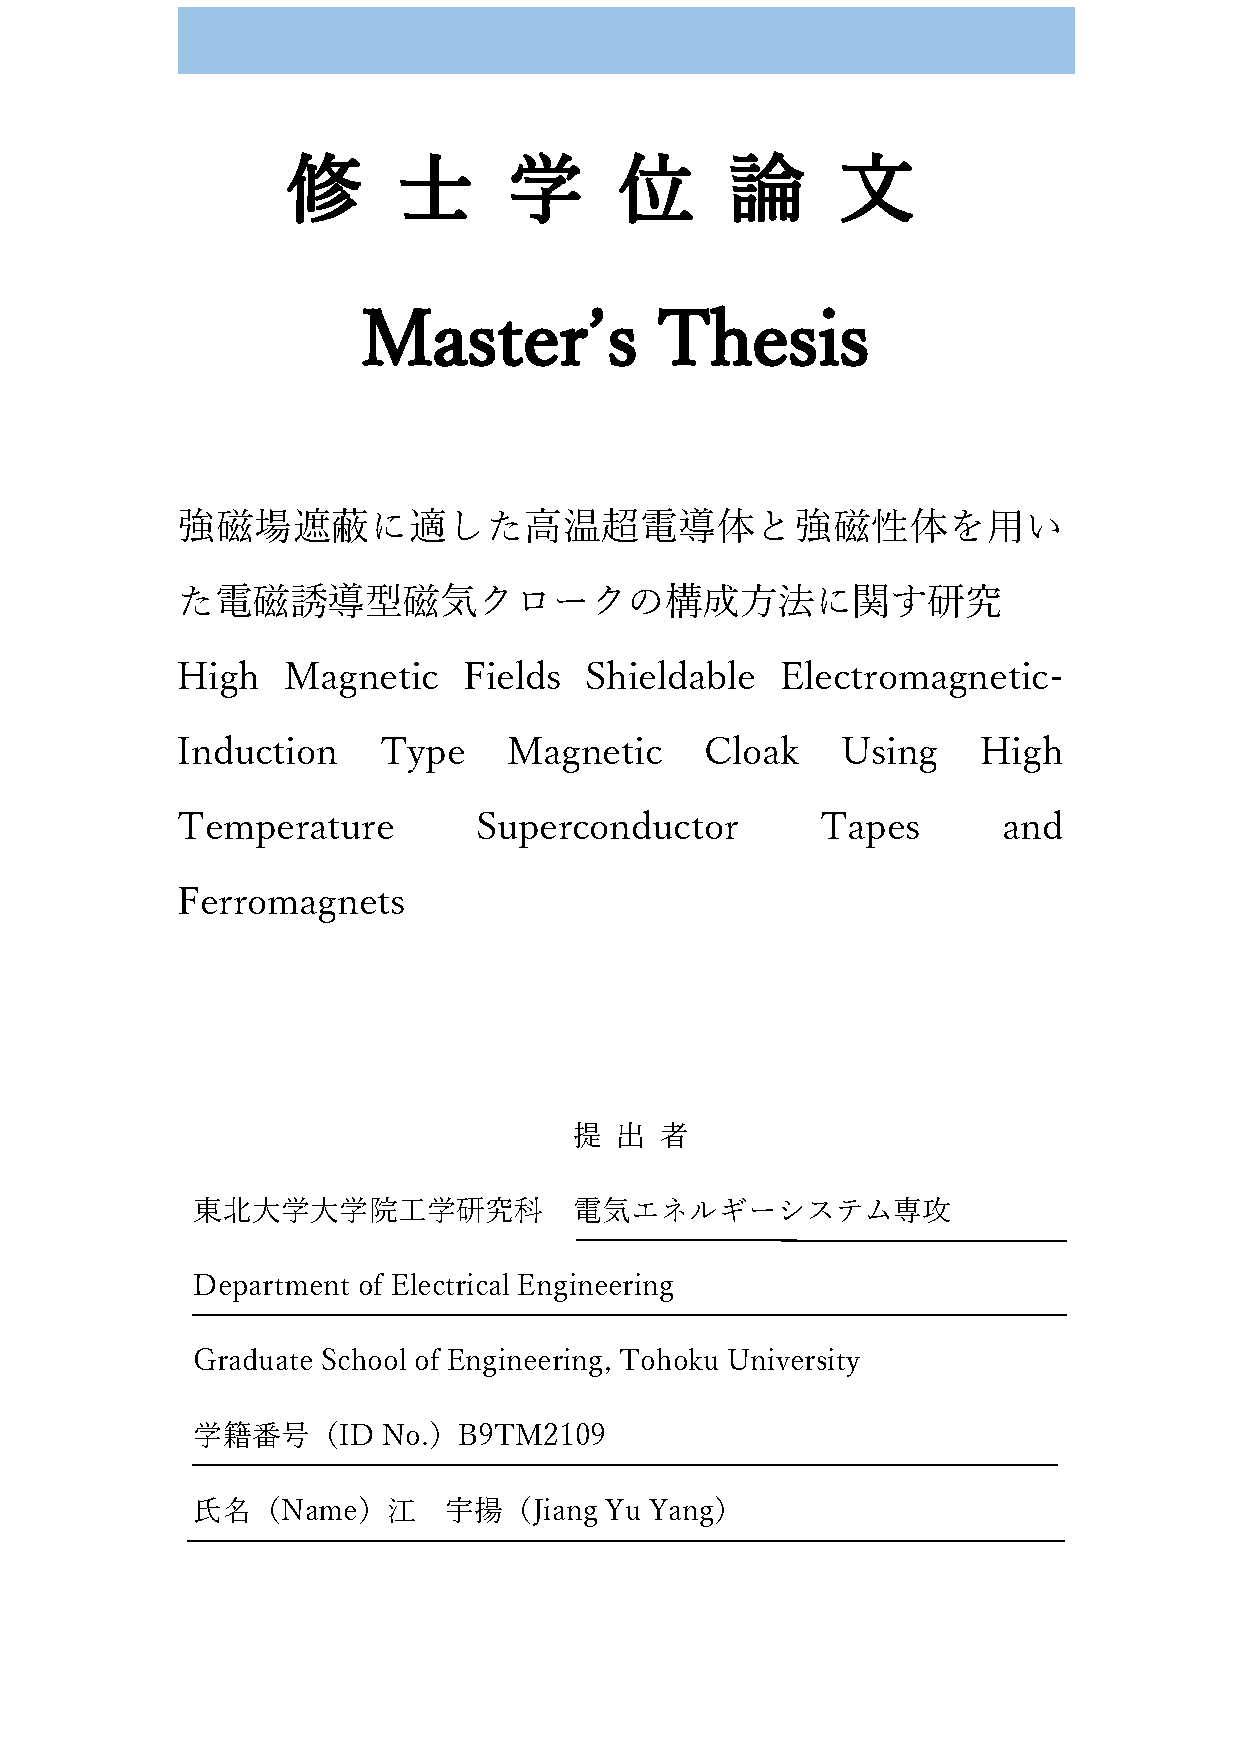
\includepdf[]{./tohokuTitlePage.pdf}
\begin{titlepage}

  \begin{table}[H]
    \centering
    \begin{tabular}{|l|l|}\hline
      Advising Professor at Tohoku Univ. & Professor Tsuda Makoto\\\hline
      Research Advisor at Tohoku Univ. & Assistant Professor Nagasaki Yoh\\\hline
      Dissertion Committee Members & O Tsuda Makoto \\
      (Name with "O" is the Chief Examiner) & 1. Ando Akira, \\
      &2. Yashima Masafummi\\\hline
      &\\
      Author's Profile & \\\hline
      Name & Jiang Yu Yang\\\hline
      Date of Birth & Mar. 18, 1995\\\hline
      Nationality & Taiwan\\\hline
      &\\
      Curriculum Vitae&\\\hline
      From April 1, 2015 to March 25, 2019 & School of Electrical Engineering, Tohoku Univ.\\\hline
      From April 1, 2019 to March 25, 2021 & Graduate School of Electrical Engineering, Tohoku Univ. \\
      &(Master's Program)\\\hline
    \end{tabular}
  \end{table}

  % \begin{table}[H]
  %   \centering
  %   \begin{tabular}{|l|l|}\hline
  %
  %   \end{tabular}
  % \end{table}

  % \begin{table}[H]
  %   \centering
  %   \begin{tabular}{|l|l|}\hline
  %     Curriculum Vitae\\\hline
  %     From April 1, 2015 to March 25, 2019 & Undergraduate School of Electrical Engineering, Tohoku University.\\\hline
  %     From April 1, 2019 to March 25, 2021 & Graduate School of Electrical Engineering, Tohoku University. \\(Master's Program)\\\hline
  %   \end{tabular}
  % \end{table}


\end{titlepage}


\setcounter{tocdepth}{3}
\tableofcontents
% adjust line space
\baselineskip=8mm
\newpage


\section{Introduction}
% section 1 Introduction
\subsection{Background}
Although the production of ultra-high magnetic fields above several tens of Tesla has been achieved these years\cite{1_1_1},
shielding of such high fields of Tesla order still remains a challenge.
Magnetic field shielding systems are generally implemented by using ferromagnets, such as Cobalt and Ferrite.
However, the magnetic flux desity of such ferromagnets becomes saturated around several hundreds mT,
causing them unavailable of shielding Tesla order fields.
Another magnetic shielding system commonly used in MRI systems generates inversed field actively to shield the original field.
While this system is feasible on shielding magnetic fields up to several Tesla,
since it is active, extra power supply is needed and the energy consumption would be enormous.
To expand the potential of high magnetic field applications,
a passive shielding system capable of shielding high magnetic fields is required.
But first, in order to clarify constraints and design principles,
we have targeted the field generated in Space Radiation Superconducting Shields(SR2S) and dedicated to develope a high magnetic field adaptable shielding system for such scheme.

To reduce the risk of exposure induced cancer for astronauts participating in International Space Station or other space missions,
attempts to use high magnetic fields to prevent the space radiation have been conducted.
The concept is similar to the geomagnetism from the Earth,
which generates a high magnetic field from the north or the south pole to divert the cosmic ray coming from deep space by the Lorentz force.
A schematic diagram is shown in Fig. \ref{fig:SR2S}.
The concept is quite straightforward,
and the magnitude of the magnetic field needed to shield the cosmic ray has been studied by multiple projects.
Many of them have reported a result of 1$\sim$8T magnetic field being generated around the spacecraft \cite{1_1_2}$\sim$\cite{1_1_5}.
In such condition, a magnetic field shielding system would be required to prevent the strong field penetrating into the spacecraft
causing unintentional side effects on human bodies and electrical equipments.
Moreover, the disturbance of the external fields should be taken into consideration as well.
In SR2S, the external strong field is used to divert cosmic rays and shouldn't be weakened by the magneitc field shielding system.
The property not to disturb external field is more widely required rather than only occurs in the SR2S case.
For instance, in the case of MRI, the strong field is used to conduct delicate medical investigation,
and thus the stability and homogeneity of which should be considered the first priority.
Since external high fields to be shielded are often producted intentionally for specific application reasons,
minimum disturbance of external fields is required for any high field shielding system.
\begin{figure}[H]
  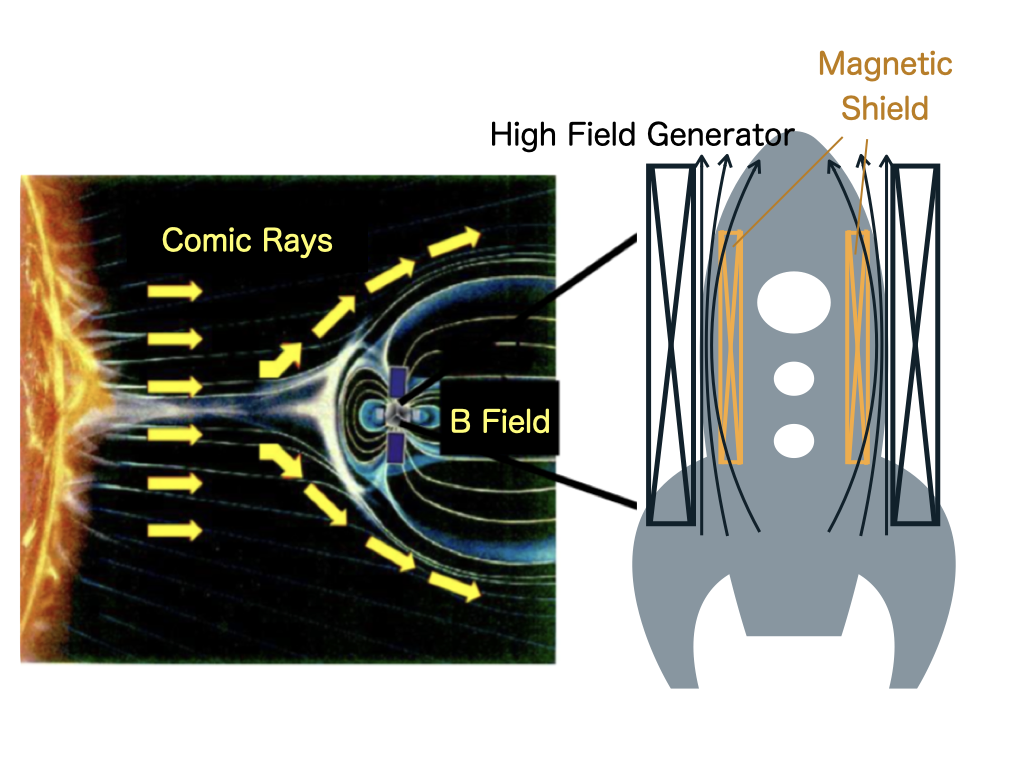
\includegraphics[width=18cm, bb=9 9 900 700]{./section1Introduction/solar.png}
  \caption{A schematic diagram of the comic ray shielding system and targeted magnetic field shielding system. }
  \label{fig:SR2S}
\end{figure}
\begin{figure}[H]
  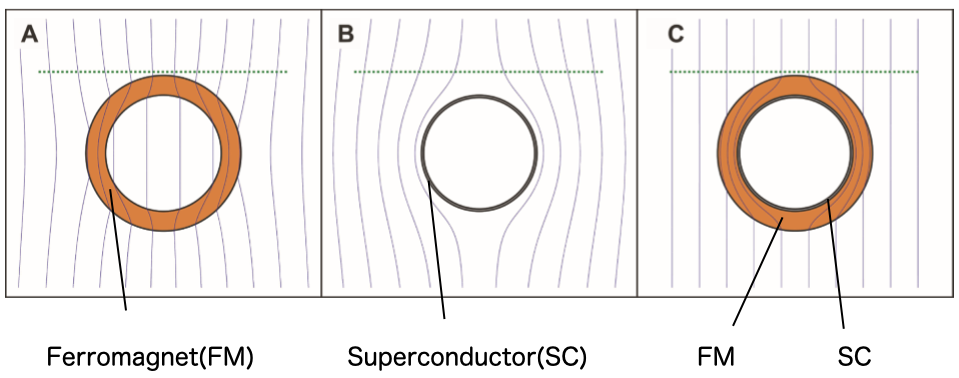
\includegraphics[width=18cm, bb=9 9 900 350]{./section1Introduction/cloak.png}
  \caption{The magnetic flux distribution when (A) a magnet, (B) a superconductor ring and (C) a manetic cloak is placed in a stable magnetic field.}
  \label{fig:cloak}
\end{figure}

In order to achieve the goal of shielding high magnetic field while not disturbing external fields,
we have introduced a new shielding system of which the concept comes from the magnetic cloak proposed by Fedor G. et al.\cite{1_1_6}.
A magnetic cloak consists of superconductor and ferromagnet in a double-layered cylindrer shape.
Generally, a ferromagnet has the property of attracting the magnetic flux while a superconductor owns the property of excluding the magnetic flux, the so called diamagnetism.
Fedor has shown that by combining the two materials which have the opposite effects,
eliminating the internal magnetic flux while not altering external fields can be achieved simultaneously.
This property is called "cloak" on magnetic fields, the concept is shown in Fig. \ref{fig:cloak}.
However, since the model relies on the Meissner effect to exclude to magnetic flux,
adaption on high magnetic fields is infeasible.
In fact, in Fedor's pape, it has been claimed to be effective up to 40 mT, which is far beyond the goal of shielding fields in several Tesla level.


In contrast, we took the idea of combining superconductors and ferromagnets and reform the construction to develope a passive magnetic cloak
which is suitable for shielding high magnetic fields on several Tesla level,
with expected scalability to further more.
In this thesis, the studies of the effectiveness and the optimized construction of the new magnetic cloak would be denoted
from various perspectives carried out by simulation and experiments.

\newpage
\subsection{High Magnetic Fields in Space Radiation Superconducting Shields}
The risk from space radiation exposure is an important concern for astronauts participating in International Space Station(ISS) missions.
Recently it has been reported that astronauts participated in at least 1 year ISS missions near solar minimum risk several percent exposure induced cancer.
For the sake of space advancement, shielding equipments of comic rays are required.

To prevent the penetration of the comic rays, many researches have been conducted.
The concept is similar to the geomagnetism from the Earth,
which generates a strong magnetic field from the North pole, covering the whole atmosphere.
Since most of the comic rays are positive charges, they tend to roll along the magnetic flux due to the Lorentz force, $F = v\times B$.
This infers that if the magnetic field is strong enough and placed properly,
it is able to divert the comic ray and work as a radiation shielding equipment.

Several projects have been set up to reproduce this mechanism on a spacecraft.
Many of them have reported a result of generating magnetic field among $1\sim8$ T on the surroundings \cite{1_1_2}$\sim$\cite{1_1_5}.
To make the system clear, a schematic diagram of the equipment is represented in Fig. \ref{fig:SR2SwithoutShielding}.
A high magnetic field of several Tesla generated along the long axis of the spacecraft spreads into the open space,
forming a magnetic wall to stop the comic ray from penetraing.
Although this system is said to be working well on diverting radiation, some magnetic shielding system is needed to protect electrical equipments from exposure of the high field.
In our research, rather than recalculate parameters or doing further studies of the comic ray shielding system,
we have left the detail of it unvarified and focused on developing a magnetic field shielding system suitable for this scheme.
\begin{figure}[H]
  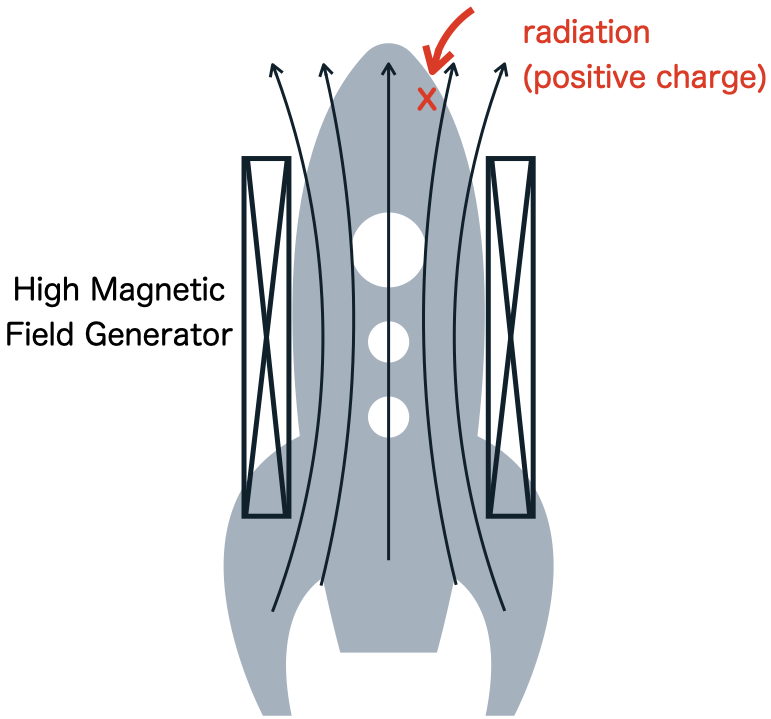
\includegraphics[width=18cm, bb=9 9 900 900]{./section1Introduction/SR2SwithoutShielding.png}
  \caption{A schematic diagram of the  comic ray shielding system using high magnetic fields. }
  \label{fig:SR2SwithoutShielding}
\end{figure}


\newpage
\subsection{Difficulties of Shielding High Magnetic Fields}
The conventional method used in magnetic shielding is using ferromagnets,
which are known to have a strong relative permeability of 1000 to several hundreds of thousand.
When imposed by some external field, magnetization $M$ with almost opposite direction against $H$ field will be induced.
With such high permeability, induced magnetization in ferromagnet becomes the dominant term in $B = \mu H + M$,
causing the $B$ field to divert significantly in the surroundings of the magnet.

Consider a hollow cylinder placed in a stable uniform field, shown in Fig. \ref{fig:FM}.
\begin{figure}[H]
  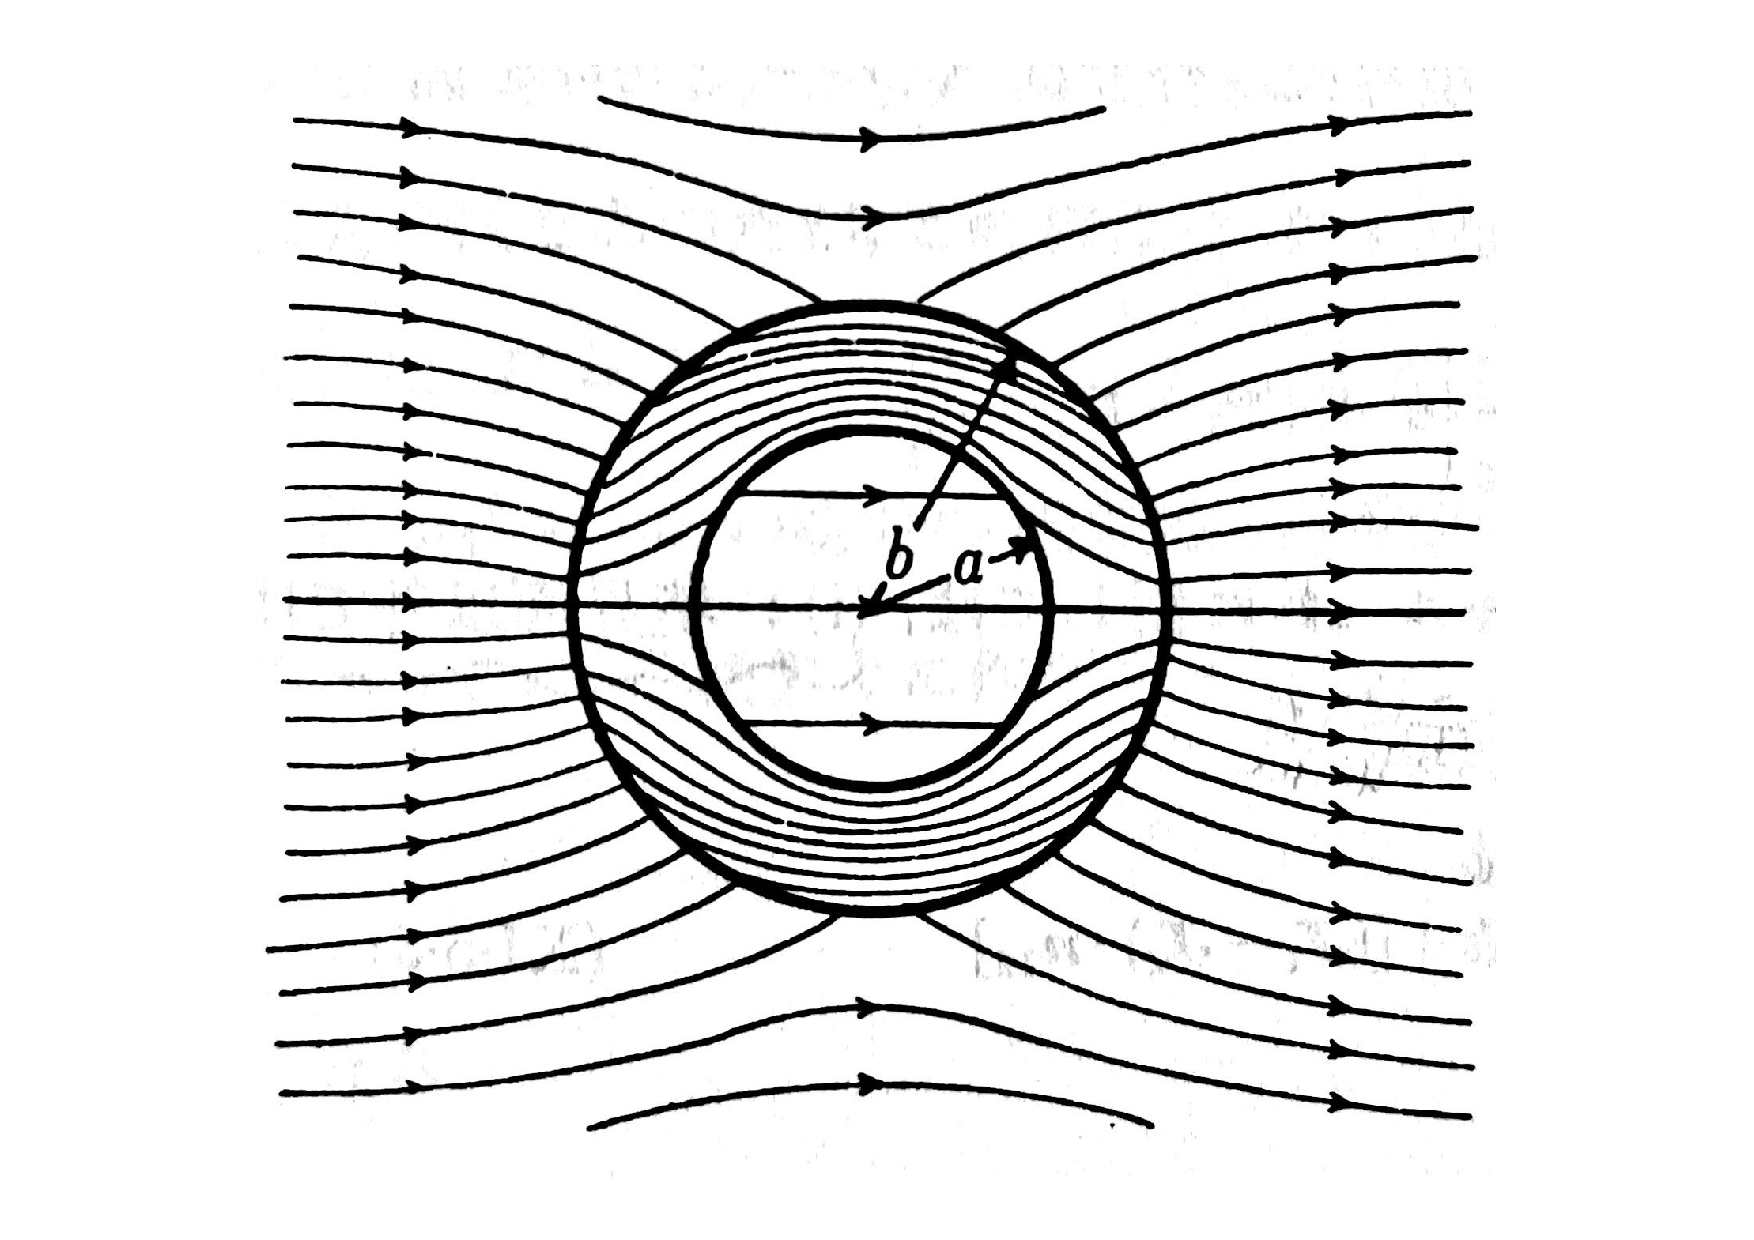
\includegraphics[width=18cm, bb=9 9 900 600]{./section1Introduction/FM.pdf}
  \caption{The $B$ field distribution near the cylinder placed in an uniform stable field \cite{1_1_7}.}
  \label{fig:FM}
\end{figure}
\begin{table}[H]
  \centering
  \caption{Shielding effects under various magnet thickness(a/b) and relative permeability($\mu_r$).}
  \label{tab:FM}
  \begin{tabular}{cc|rrrrr}\hline\hline
    a/b &  & 0.99 & 0.8 & 0.6 & 0.4 & 0.2\\\hline
    $H_{internal}/H_{external}$ & $\mu_r = 100$ & 3/5 & 1/12 & 1/18 & 1/22 & 1/23 \\
    $H_{internal}/H_{external}$ & $\mu_r = 1000$ & 3/23 & 1/109 & 1/175 & 1/209 & 1/221 \\\hline\hline
  \end{tabular}
\end{table}
Affected by the induced magnetization $M$, the magnetic flux in the magnet part is reinforced and that in the internal space is reduced.
The internal field is shown in detail in Tab. \ref{tab:FM}, along with different permeability.
From Tab. \ref{tab:FM},
increasing the permeability or the thickness of the magnet yields a better shielding effect.
As well, elimination near 99\% in the interior space can be achieved using magnets with relative permeability of several thousands,
which is a common value for modern ferromagnetic materials.
This method is often known as the "magnetic screening".

Due to its simplicity, magnetic screening is widely used in industry, especially in electrical devices like smartphone.
However, common ferromagnetic materials like ferrite can only provide a limited magnetization up to 700 mT,
making the magnetic screening to fail on high imposed fields as several Tesla level.
This is the main difficulty on high magnetic field shielding.

Besides, since the generation of high magnetic fields itself is difficult, they are often produced intentionally for application reasons.
In SR2S they are applied to prevent comic rays, in MRI they are used to conduct detailed examination of human bodies,
in biological or physical regions they surves as a means of trigger of new phenomena, etc.
When a magnetic shielding system is inserted in the neighborhood of these high fields,
those fields may be disturbed.
In Fig. \ref{fig:cloak}(A), it is clear that the field near the ferromagnet is disturbed due to the induced magnetization.
In Fig. \ref{fig:cloak}(B), disturbance on the external field due to the diamagnetism of the superconductor can also be observed.
Consider the application of these fields, the stability of which should be given the first priority and thus
the property that magnetic shielding systems implemented afterwards not altering the external field is required.
In spite of such demand, conventional shielding methods fail to meet the needs, leaving it an open challenge.

As describe in section 1.1, the property that internal field is eliminated while the external field distribution remains unchanged
is known as "cloak" on magnetic fields.
This concept has started to become possible theese years using anisotropic, spatially inhomogeneous, or singular values of magnetic permeability \cite{1_1_8}$\sim$\cite{1_1_11}.
A further simplified model has been proposed in Fedor's paper \cite{1_1_6} in 2012, in which ferrormagnets and low-temperature superconductors are used.


However, all of them are neither designed for high magnetic field application,
nor capable to shield fields of several Tesla.
With high magnetic field application grow,
a magnetic cloak capable fo operating in high field is required.
To achieve such system, the problem of magnetization saturation under high fields should be overcame
while disturbance of the external field is eliminated,
which seems extremely difficult.


\newpage
\subsection{Purpose of the Study}
To expand the potential application of high magnetic fields of several Tesla,
a magnetic cloak adaptable to high fields is required.
In detail, the cloak must satisfy 2 properties:
\begin{enumerate}
  \item Able to shield magnetic fields of several Tesla.
  \item Have a limited disturbance on external fields.
\end{enumerate}

In this study, in order to clarify the constraints and real-world application,
we have focused on the SR2S project in space usage,
and set up the goal to be the followings, which is slightly different from the above:
\begin{enumerate}
  \item Able to shield 1 T magnetic field.
  \item Have a limited weakening effect on the external field.
\end{enumerate}
For the 1st property, we have taken into consideration the equipment in our laboratory.
Since the S2RS project generates $1\sim 8$T fields and the ferromagnet applied in this study owns a saturation field of 700 mT,
this setting is considered sufficient to testify the proposed magnetic cloak.
For the 2nd property, since the magnetic field in the SR2S project is used to divert the comic ray,
the external field being weakened should be consider a larger issue than being reinforced.
A weakened area of the external field will allow the comic rays penetrating into the spacecraft causing potnetial damage on human bodies while a strengthened area of the external field will not trigger any fatal problem.
For convinience, we have changed the 2nd property to be concentrated in preventing the external field from weakening.

Through this thesis, a new designed magnetic cloak suitable to work in high fields will be introduced,
with which the effectiveness and optimal construction will be described further in the following sections.


\newpage
\subsection{Construction of This Thesis}
In section 2, we first describe our proposal of overcoming the difficulties of shielding high magnetic fields.
The concept, construction, how it works along with the improvement from the conventional magnetic cloak are denoted.

In section 3, the evidence on the expectable capability of achieving cloak on high magnetic fields are shown.
To proof the ability of shielding effect,
we have conducted a series of experiments on the scaled down model.
Since each of the experiment have been designed for specific purpose,
the theory, experimental set up, results and discussion are described relatively.

In section 4, after the effectiveness have been revealed, the optimized construction of the position of superconductor tapes and ferromagnets are stated with detailed simulation.
The simulation are conducted by advance methods such as the Finite Element method and modern optimization algorithms which might be unfamiliar to readers who don't have a background on algorithm region.
Despite that the full detail of theese analysis is beyond the scope of this thesis,
we have been dedicated in explaining the story step by step with information described as detailed as possible.
If it is found difficult to under stand, please refer to the articles in reference.

In section 5, the result done on 1 T environment using the model near full scale is stated and discussed.
Finally, the whole thesis is summaried in section 6.


\newpage
\begin{thebibliography}{11}
  \bibitem{1_1_1} N. Miura, T. Goto, K. Nakao, S. Takeyama, T. Sakakibara, T. Haruyama, T. Kikuchi, "Production of ultra-high magnetic fields and their application to solid state physics", Physica B: Condensed Matter, Volume 155, Issues 1–3, Pages 23-32 (1989)
  \bibitem{1_1_2} Filippo Ambroglini1, Roberto Battiston2 and William J. Burger, "Evaluation of Superconducting Magnet Shield Configurations for Long Duration Manned Space Missions", Frontiers in Oncology, Vol. 6, p. 97 (2016)
  \bibitem{1_1_3} R. Musenich, V. Calvelli, S. Farinon, W. J. Burger, R. Battiston, "Space Radiation Superconducting Shields", Journal of Physics: Conference Series 507 032033 (2014)
  \bibitem{1_1_4} Westover SC, Meinke RB, Battiston R, Burger WJ, Van Sciver S, Washburn S, et al. Magnet Architectures and Active Radiation Shield Study. NASA Institute for Advanced Concepts (NIAC) Phase 1 Final Report (2012)
  \bibitem{1_1_5} Battiston R, Burger WJ, Calvelli V, Musenich R, Choutko V, Datskov VI, et al. Superconductive Magnet for Radiation Shielding of Human Spacecraft. (2011)
  \bibitem{1_1_6} Fedor Gömöry et al., "Experimental Realization of a Magnetic Cloak", Science 335, 1466 (2012)
  \bibitem{1_1_7} 竹山 説三, "電磁気學現象理論", p. 269, 丸善 (1949)
  \bibitem{1_1_8} 1. J. B. Pendry, D. Schurig, D. R. Smith, Science 312, 1780 (2006)
  \bibitem{1_1_9} U. Leonhardt, Science 312, 1777 (2006)
  \bibitem{1_1_10} A. Greenleaf, M. Lassas, G. Uhlmann, Physiol. Meas. 24, 413 (2003)
  \bibitem{1_1_11} A. Alù, N. Engheta, J. Opt. A Pure Appl. Opt. 10, 093002 (2008)
\end{thebibliography}


\newpage
\section{Proposal: Electromagnetic-Induction Type Magnetic Cloak using High Temperature Superconductor Tapes and Ferromagnets}
% section 2 Proposal
In this chapter, the fundamental macroscopic concepts of superconductivity, Meissner effect, ferrormagnetism,
and the modern high temperature superconductor tape are described in detail.
With only limited acknowledge of Maxwell equation is assumed, readers who are new to this region should be able to understand unproblematically.
For advanced readers who is familiar to superconductivity, you are welcome to skip to the magnetic cloak parts.

In the later sections of this chapter, we first give an introduction on the conventional magnetic cloak,
how the concept works and the potential issue occured.
Then the description of the proposed new Electromagnetic Induction type magnetic cloak follows.


\newpage
\subsection{Superconductor}
Since its first discover in 1911, superconductor materials have been surprising scientists with the rapid improvement year after year.
In 1911, short after the liquefaction of helium had been achieved, Kamerlingh Onnes found that the electrical resistance of mercury dropped extremely under a low temperature of 4.2 K \cite{2_1}.
This phenomanen is later discovered to appear in several metals, and is named "superconductivity" by Kamerlingh.
The result of the experiment conducted on mercury is shown in Fig. \ref{fig:mercury}.
\begin{figure}[H]
  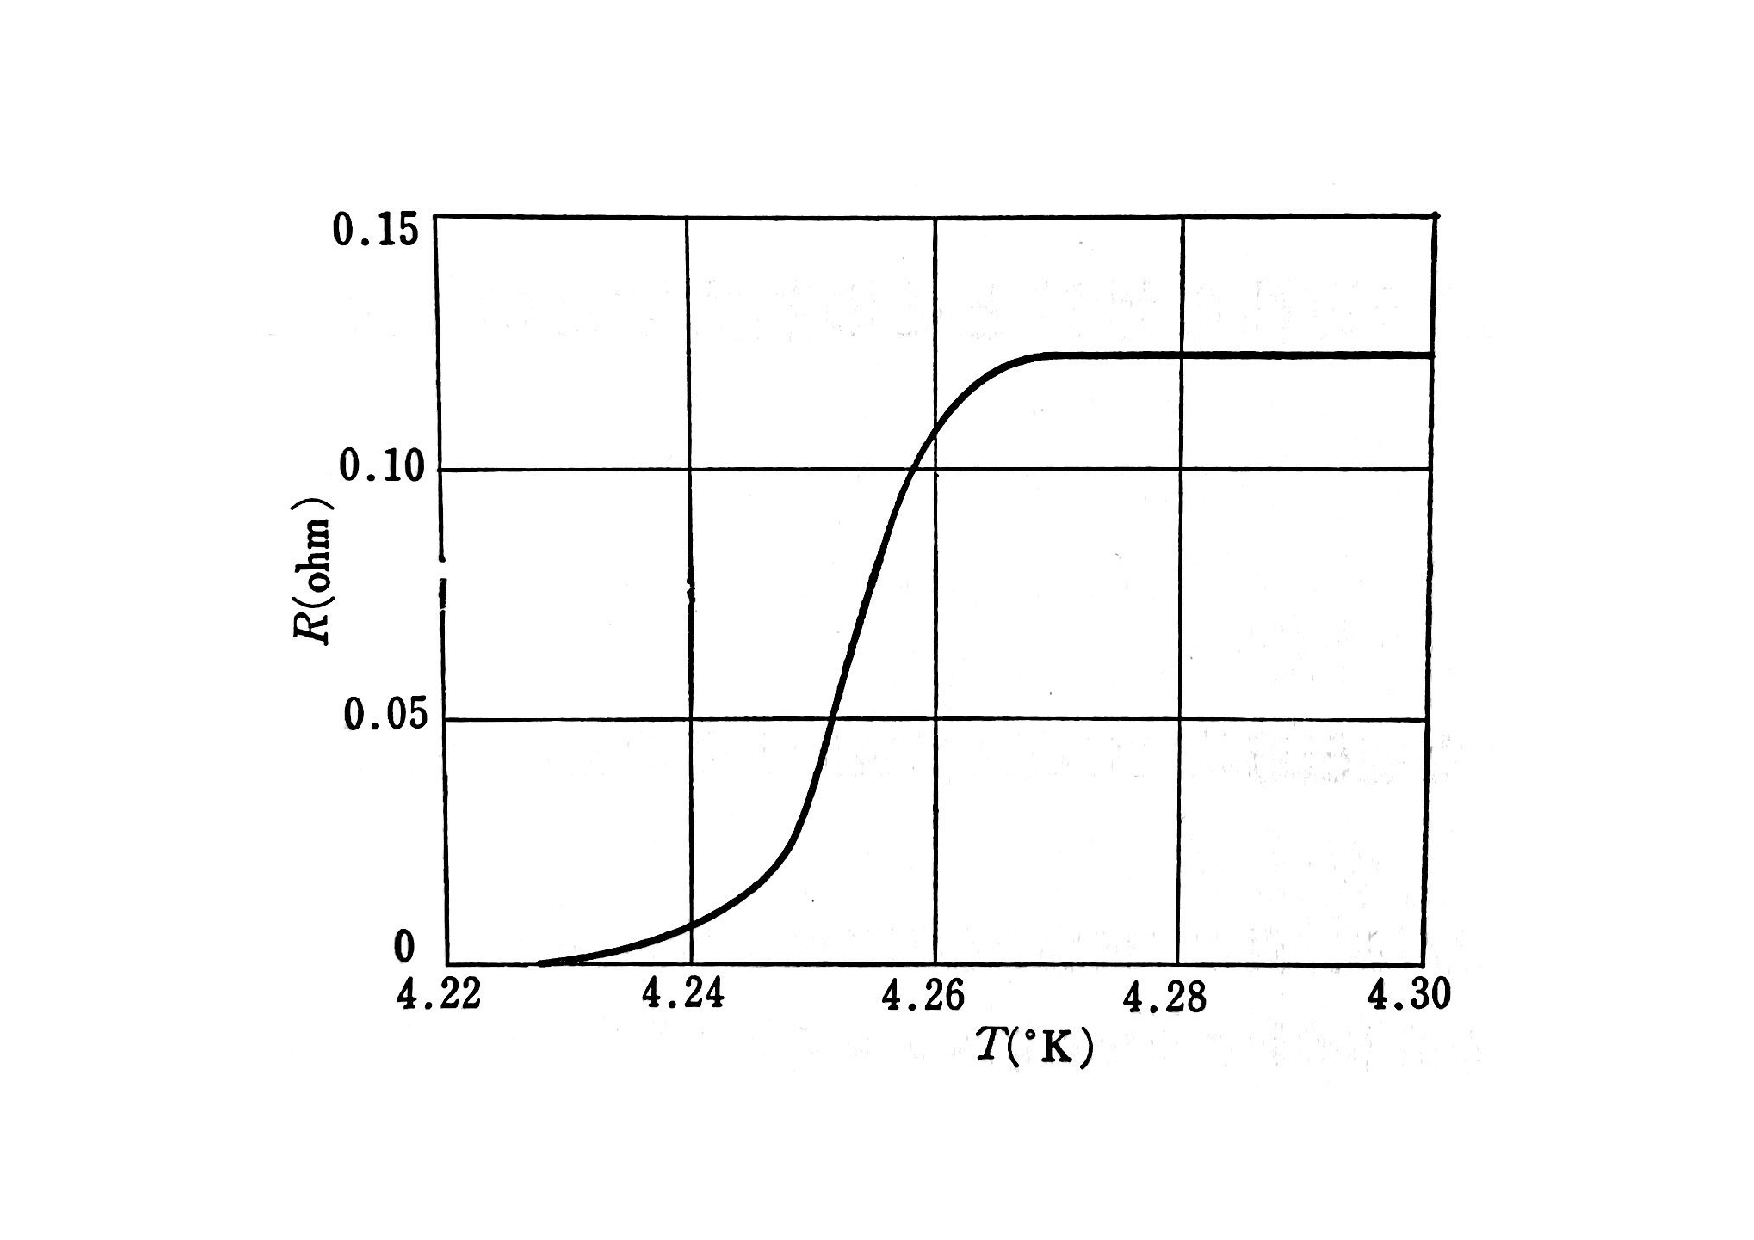
\includegraphics[width=20cm, bb=9 9 900 500]{./section2Proposal/mercury.pdf}
  \caption{Temperature-Resistance relationship on mercury \cite{2_2}.}
  \label{fig:mercury}
\end{figure}

Additionally, Kamerlingh has also found that the superconducting state can be corrupted if imposed by certain magnetic fields of tens of mT. The magnetic field in which a material can tolerate to retain its superconducting state is called the "critical field".
The critical field is often related to the temperature.
In Fig. \ref{fig:H-T}, an example of the critical field - temperature curve is shown.
From which, we can see that most of the conventional metals only have the ability to maintain superconductive under a very low temperature of several Kelvin, and tens of mT of imposed field.
This indicates that the superconducting state is a relatively unique state which only occurs in extreme conditions and can be corrupted easily.
\begin{figure}[H]
  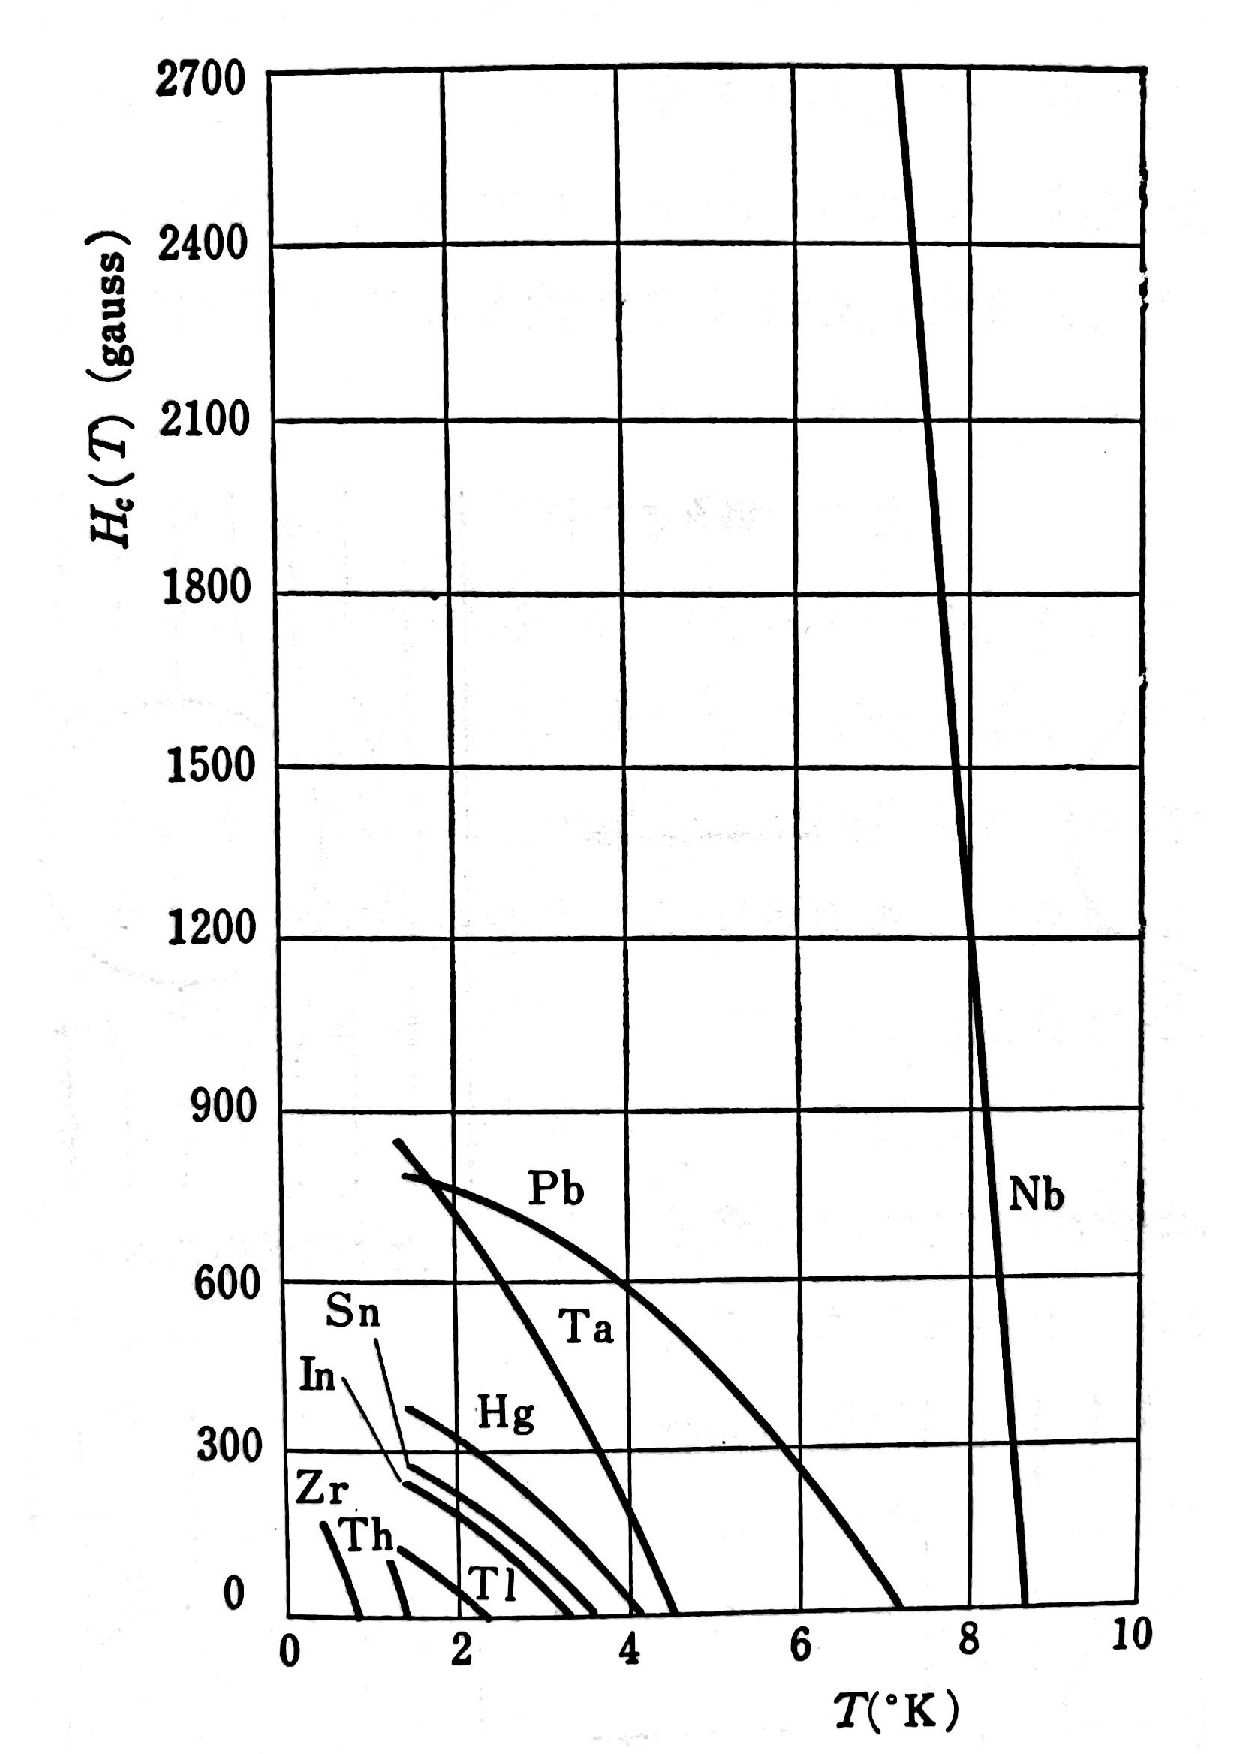
\includegraphics[width=15cm, bb=9 9 900 900]{./section2Proposal/H-T.pdf}
  \caption{Critical Field(H) - Temperature curves observed on several metals \cite{2_3}. Note that 10 Gauss = 1 mT.}
  \label{fig:H-T}
\end{figure}

Note that superconductivity is a special state into which some specific material can transit under certain conditions,
rather than pointing the material itself.
The transition can be concerned as a general phase transition under certain conditions occured in the environment.
To avoid confusion, we tend to use the phrase "superconducting state" instead of "superconductor" in this thesis.


\newpage
\subsubsection{Perfect Conductivity}
The fact that in the superconducting state the electrical resistance drops to an unobservable level has been varified by many experiments \cite{2_4}.
If the zero resistance can be seen as the electrical conductivity $\sigma$ being nearly infinitive,
due to Farraday's rule and ohm's rule,
\begin{eqnarray}
  \mathrm{rot}\bm{E} = \frac{\partial \bm{B}}{\partial t}\\
  \bm{J} = \sigma \bm{E}
\end{eqnarray}
we have
\begin{equation}
  \lim_{\sigma \to \infty} \mathrm{rot} \frac{\bm{J}}{\sigma} = \frac{\partial \bm{B}}{\partial t} = 0
\end{equation}
which indicates that the magnetic field $B$ doesn't change from the initial value in a superconductor.
This scheme can be realized as the "conservation of inital field",
in which the initial field means the field imposed at the exact point of time when the material went into the superconducting state.
An example about this expactation is shown in Fig. \ref{fig:perfectConductivity}.
\begin{figure}[H]
  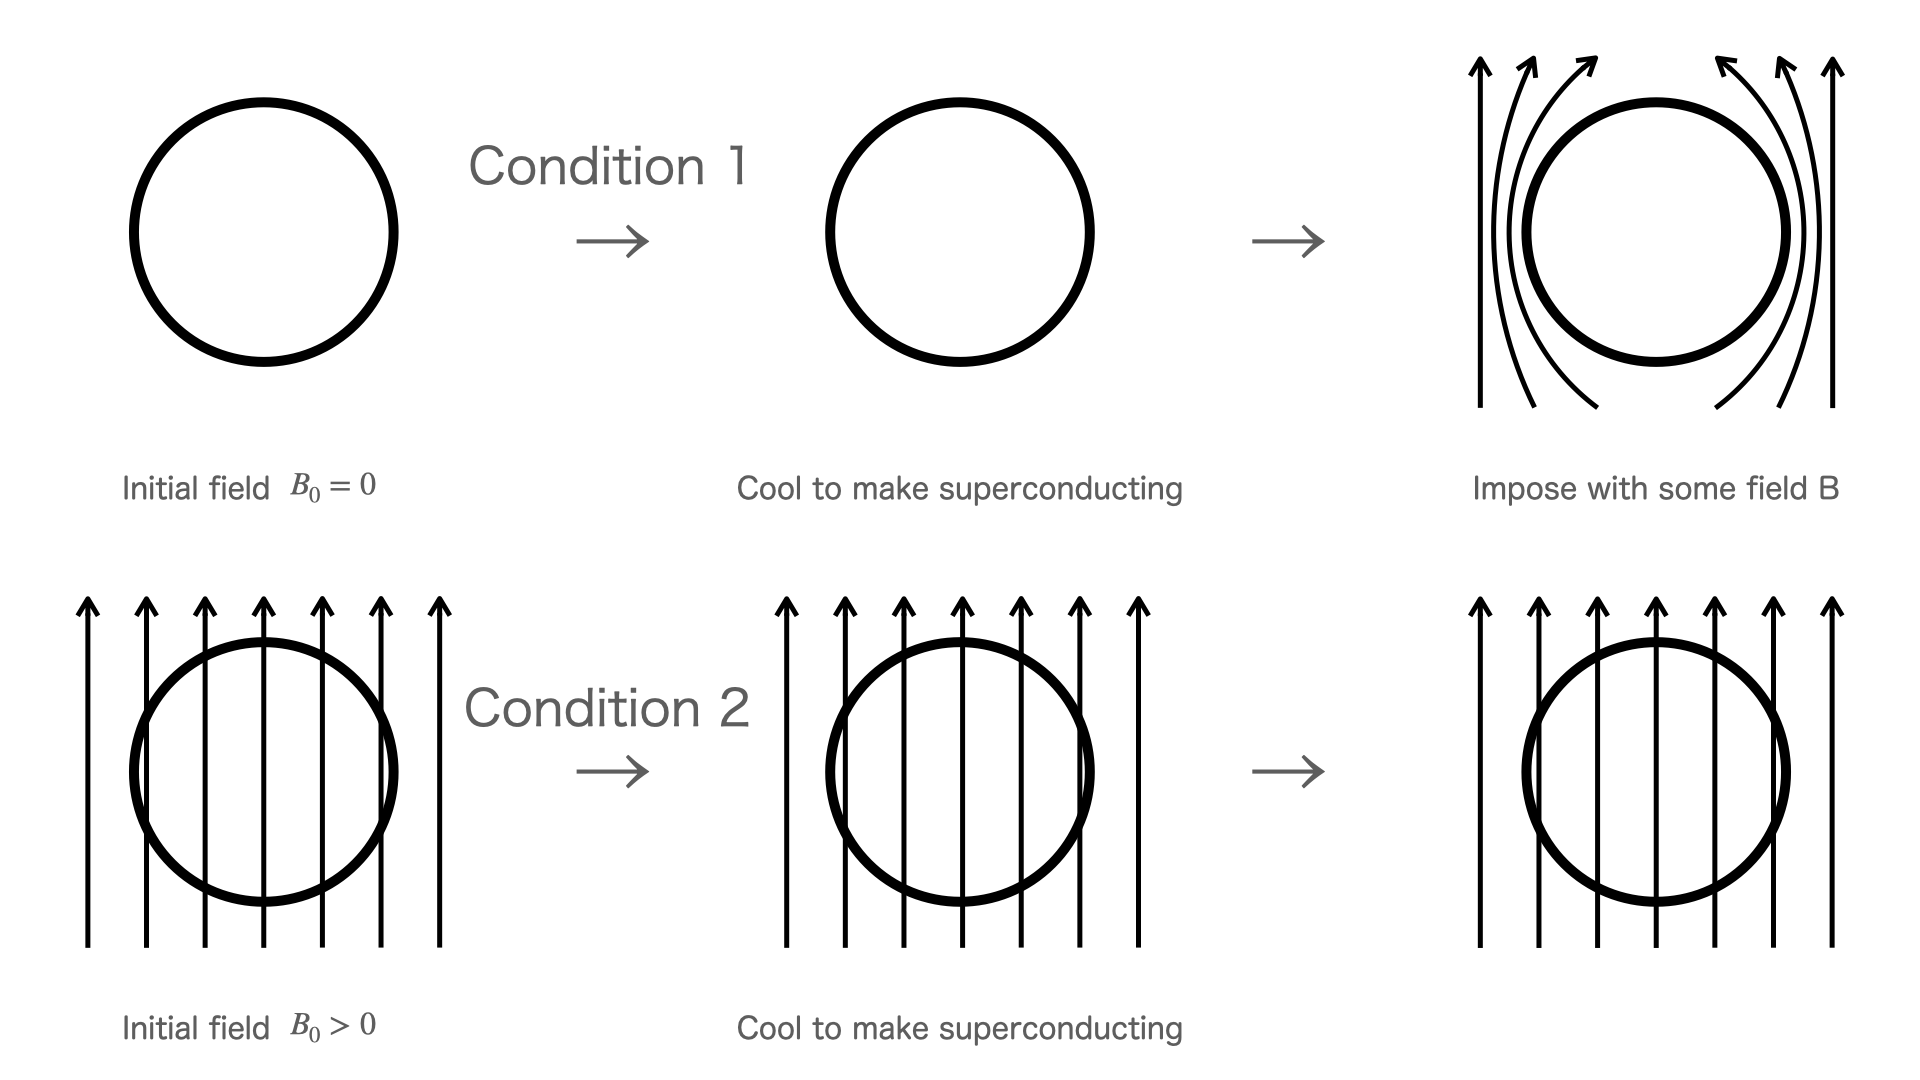
\includegraphics[width=18.5cm, bb=9 9 900 500]{./section2Proposal/perfectConductivity.png}
  \caption{The {\bf expected} magnetic field distribution around a solid ball in the normal state and superconducting state under different initial fields. \cite{2_1}}
  \label{fig:perfectConductivity}
\end{figure}
In condition 1, where the material enters its superconducting state with the initial imposed field $B_0$ being zero,
shows the conservation of zero magnetic flux when it is later imposed with certain $B > 0$.
In condition 2, where the material is first given some initial field $B_0 > 0$ before it becomes superconducting,
again should show the conservation of $B_0$ magnetic flux during all periods.
This expactation is directly derived from the Maxwell equation (3), which explains the behavior of the magnetic field in a perfect conductivity $\sigma \to \infty$ situation.
For a long period this phenomanen was believed to be actually occuring inside a superconducting material,
and many experiments have shown an imitate distribution of Fig. \ref{fig:perfectConductivity}.

If this is true, all of the possible states of the magnetic field distribution inside a superconductor must be thermodynamically balanced,
which is hard to imagine.
Though semi-equilibrium states do exists in reality such as glass at low temperature and overcooled liquid,
in a state where electrons can move without any resistance,
the achievement of such semi-equilibrium situation is difficult to explain.
In fact, instead of fully investigating the mechanism occurs in a superconducting state,
equation (3) $\frac{\partial{\bm B}}{\partial t} = 0$ only describes what would have happened assumed that the conductivity is near infinity.
Also, assurance that the Maxwell equation would hold in such state could not be made before considering the molecular interaction from the perspective of quantum mechanics.


\subsubsection{Meissner Effect (Perfect Diamagnetism)}
Not until the magnetic field distribution near a superconductor measured by Meissner and Ochsenfeld striclty in 1933 has the story changed dramatically \cite{2_5}.
In the experiment focusing on stannum,
they first imposed some parallel field and then cool it into the superconducting state.
In contrast of the expectation shown in Fig. \ref{fig:perfectConductivity},
a significant change on the magnetic field around the material was observed at the transition temperature.
The magnetic flux behaved like being removed from the superconductor,
as the one shown in Fig. \ref{fig:meissner}.
On the surface of the solid superconductor ball,
the vertical component of magnetic field became zero and the field $B$ inside disappeared.
This unexpected result has indicated that
the eigen magnetic behavior in a superconductor is
\begin{equation}
  {\bm B} = 0
\end{equation}
not
\begin{equation}
  \frac{\partial{\bm B}}{\partial t} = 0 \nonumber
\end{equation}
This phenomanen described by equation (4) is called "Meissner Effect",
and is concerned the most original property of a superconductor.
Nowadays, only when a material achieves both zero resistance and the Meissner effect can be declaimed as a superconductor.
\begin{figure}[H]
  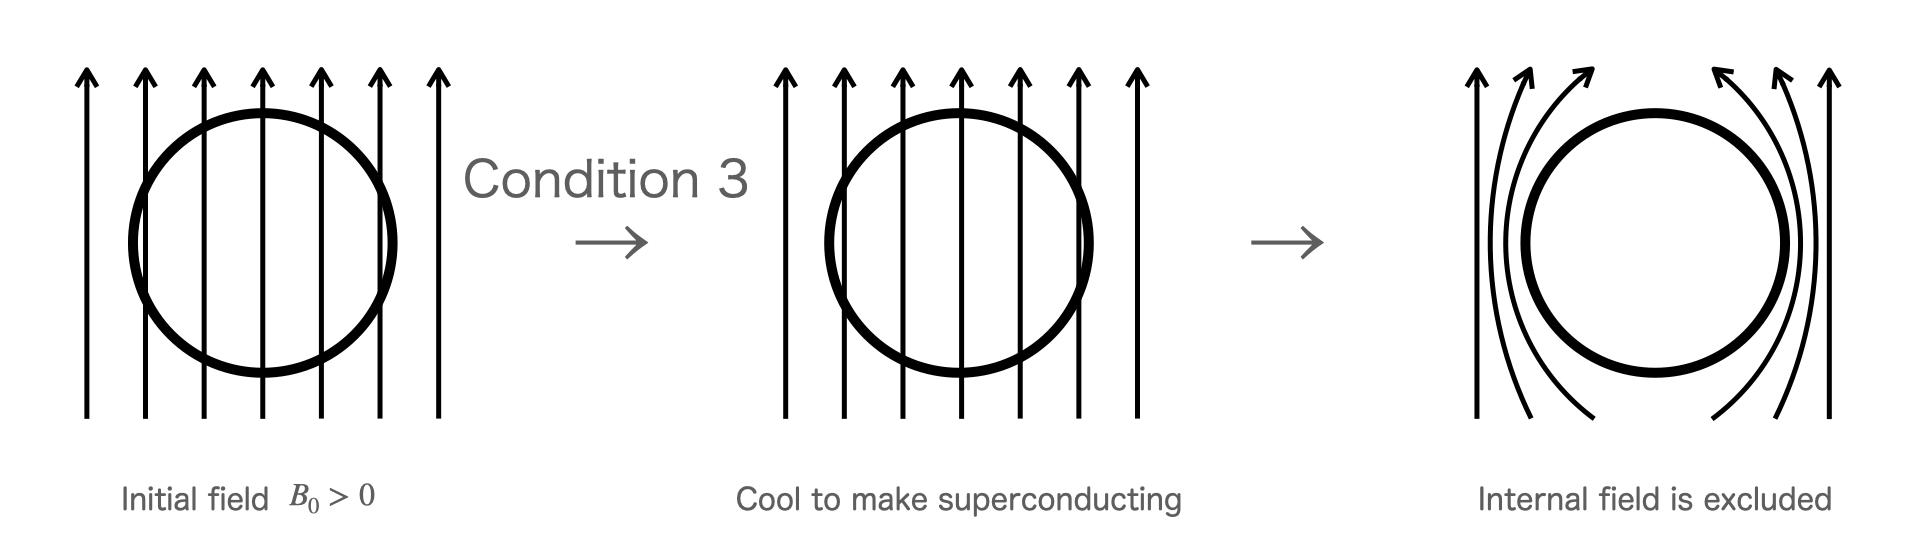
\includegraphics[width=18.5cm, bb=9 9 900 260]{./section2Proposal/meissner.png}
  \caption{The concept of Meissner effect: $B = 0$.}
  \label{fig:meissner}
\end{figure}

Why does it take scientists decades to find this phenomanen?
The Meissner effect could be obscured due to impurities in superconductor or inhomogeneous distribution of the material.
The fact that "frozen" magnetic flux in superconductor under unideal condition is observed
may be considered as the superconducting part and the normal part existing simultaneously in the material.
For instance, if the crystal of the metal is inhomogeneous, then in the superconducting state, the inhomogeneous part may distort the nearby field.
If the magnetic field density is somehow high in certain region,
the superconducting state may collapse partially,
turning the crystal into a state mixed by superconducting and normal regions.
Theese pratical conditions make the magnetic flux "locked in" some normal parts in a superconductor.

To continue, whether a normal region can exist in the superconducting state is the key difference between the so called first kind and second kind superconductor.
In an ideal (pure and homogeneous) metal, such as mercury and those been tested by Kamerlingh (see Fig. \ref{fig:H-T}),
magnetic flux is unable to penetrate it during the superconducting state due to the Meissner effect.
Consequently, theese crystals, known as the first kind of superconductor,
usually have a low critical field and a low transition temperature,
since their tolerance to external turbulence on electromagnetic and thermodynamic is poor.
In contrast, superconductors consists of complicated compounds such as CuO2 and those labeled as the High Temperature Superconductor
allow the normal region to emerge during the superconducting state.
Theese compounds, named the second kind of superconductor,
do not show the perfect Meissner effect but are capable to tolerate a much more higher field and temperature.


\newpage
\subsection{High Temperature Superconductor(HTS) Tape}
Great imporvements had been achieved these years on manufactoring superconductor having a high critical current and transition temperature.
Generally, the conventional superconductors discovered in the 1910s usually are well-known pure metals and only transit to the superconducting state in an extremely low temperature of a few Kelvins.
In 1986, J. G. Bednorz and K. A. Müller has found that superconductivity transition has occured at 30 K in the copper oxide Ba-La-Ci-O compound.
In the next few years, superconductors with transition temperature above the boiling point of nitrogen, 77 K,
are discovered in copper oxide crystals,
which allows the generation of the superconductivity more easily using liquid nitrogen.
Copper based superconductors had long been the state-of-the-art high temperature superconductor having a high transition temperature and a pratical manufactor process.
Dosens of studies had been conducted on them, until a break through on the transition temperature was made by hydrogen sulfide under extremely high pressure of 100G Pa \cite{2_8}.
In late 2020, Snider et al. has marked an record of achieving a superconductivity transition at room temperature ($14^\circ \mathrm{C}$) \cite{2_9}.
The whole timeline of the high temperature superconductor development is shown in Fig. \ref{fig:HTSs}.
\begin{figure}[H]
  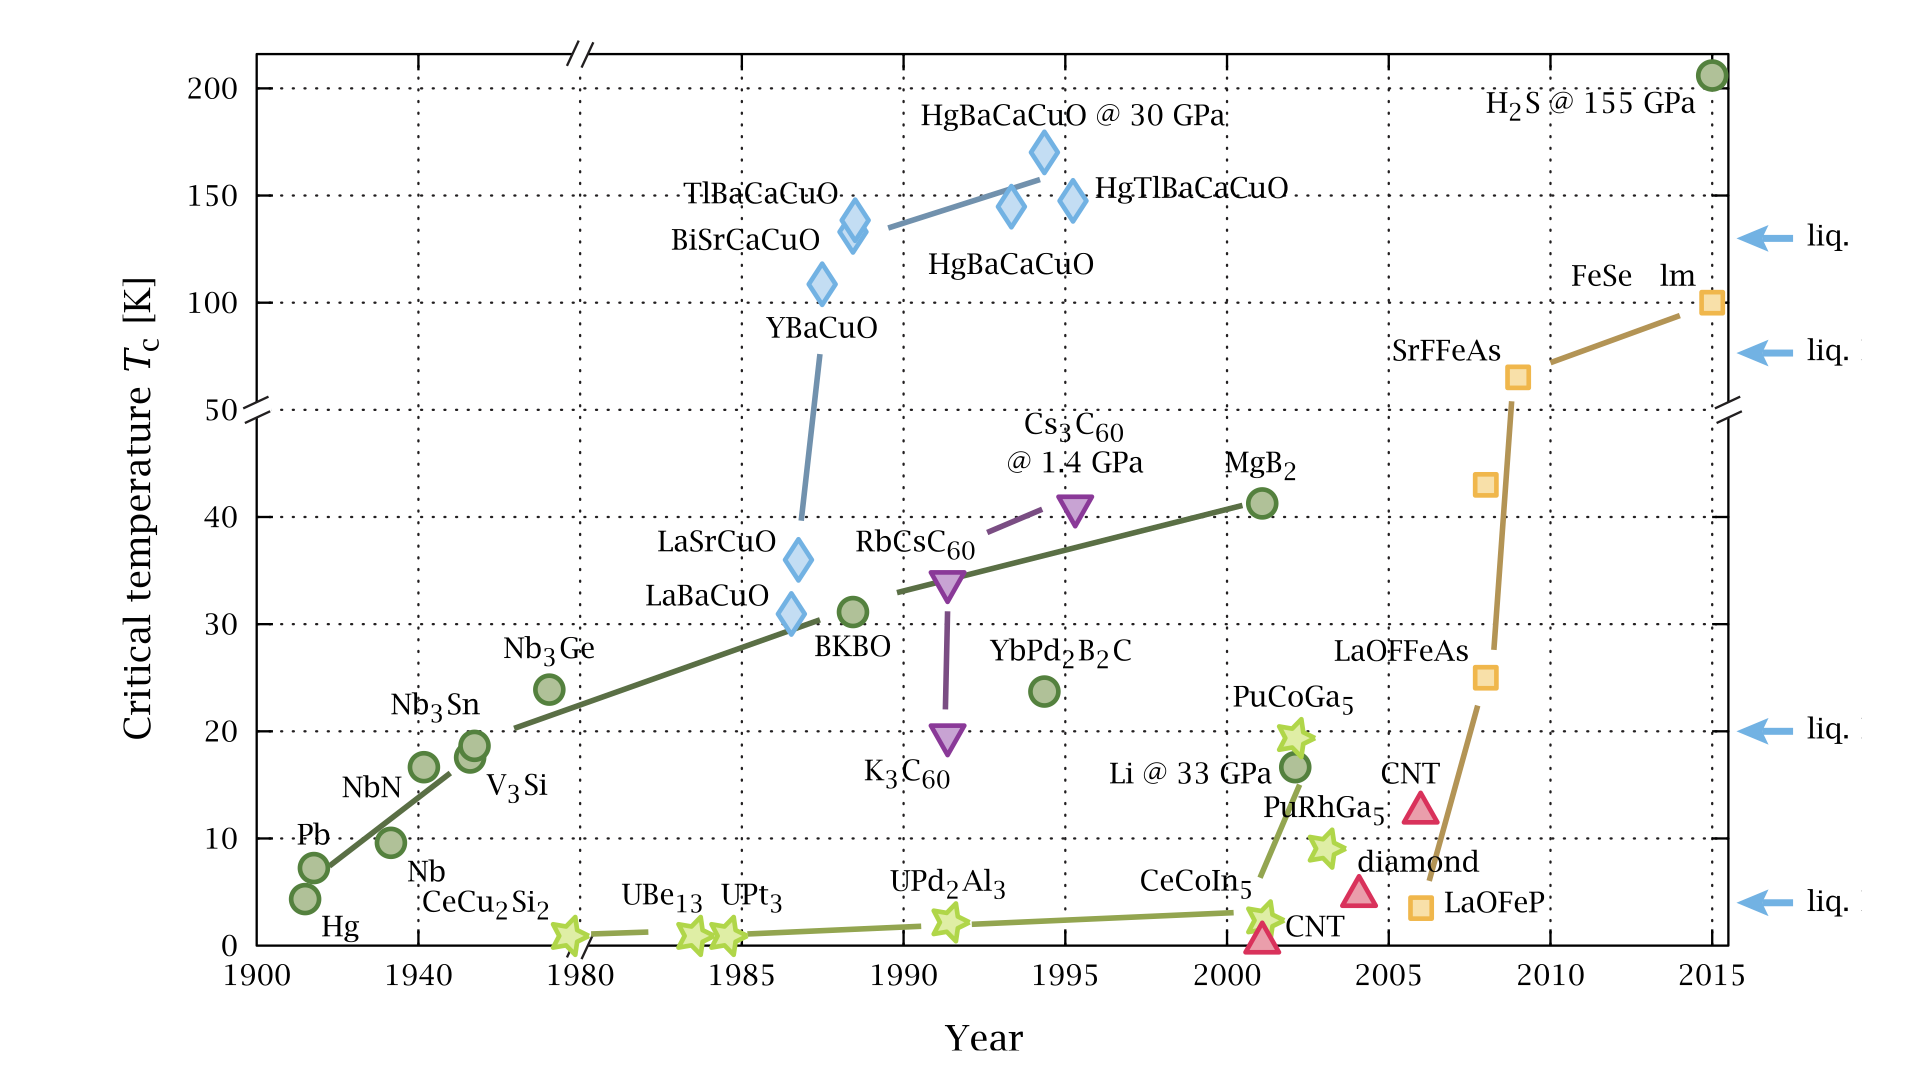
\includegraphics[width=18.5cm, bb=9 9 900 500]{./section2Proposal/HTSs.png}
  \caption{}
  \label{fig:HTSs}
\end{figure}

To avoid confusion, theese superconductors discovered after 1980s which have higher transition temperatures, tolerable on higher currents,
allow magnetic field penetration (which makes them the second kind superconductor in classification),
are often called the High Temperature Superconductor(HTS).
The superconductors discovered before then,
which have lower transition temperatures, show an ideal Meissner effect, classified into the first kind superconductor, are often called the Low Temperature Superconductor.

In our study, we use the copper oxide superconductor YBa2Cu3O7(YBCO) due to its stable supply and the availability with liquid nitrogen cooling.
The YBCO superconductor is generally manufactored in a tape form, within which electrons is able to move without resistance along the long axis.
At the production level, a pure copper or silver layer is often additionally overlaid to increase electrical stability.
The structure of the whole tape is shown in Fig. \ref{fig:Y},
and the specification of the superconductor used through this thesis is shown in Tab. \ref{tab:Y}.
\begin{figure}[H]
  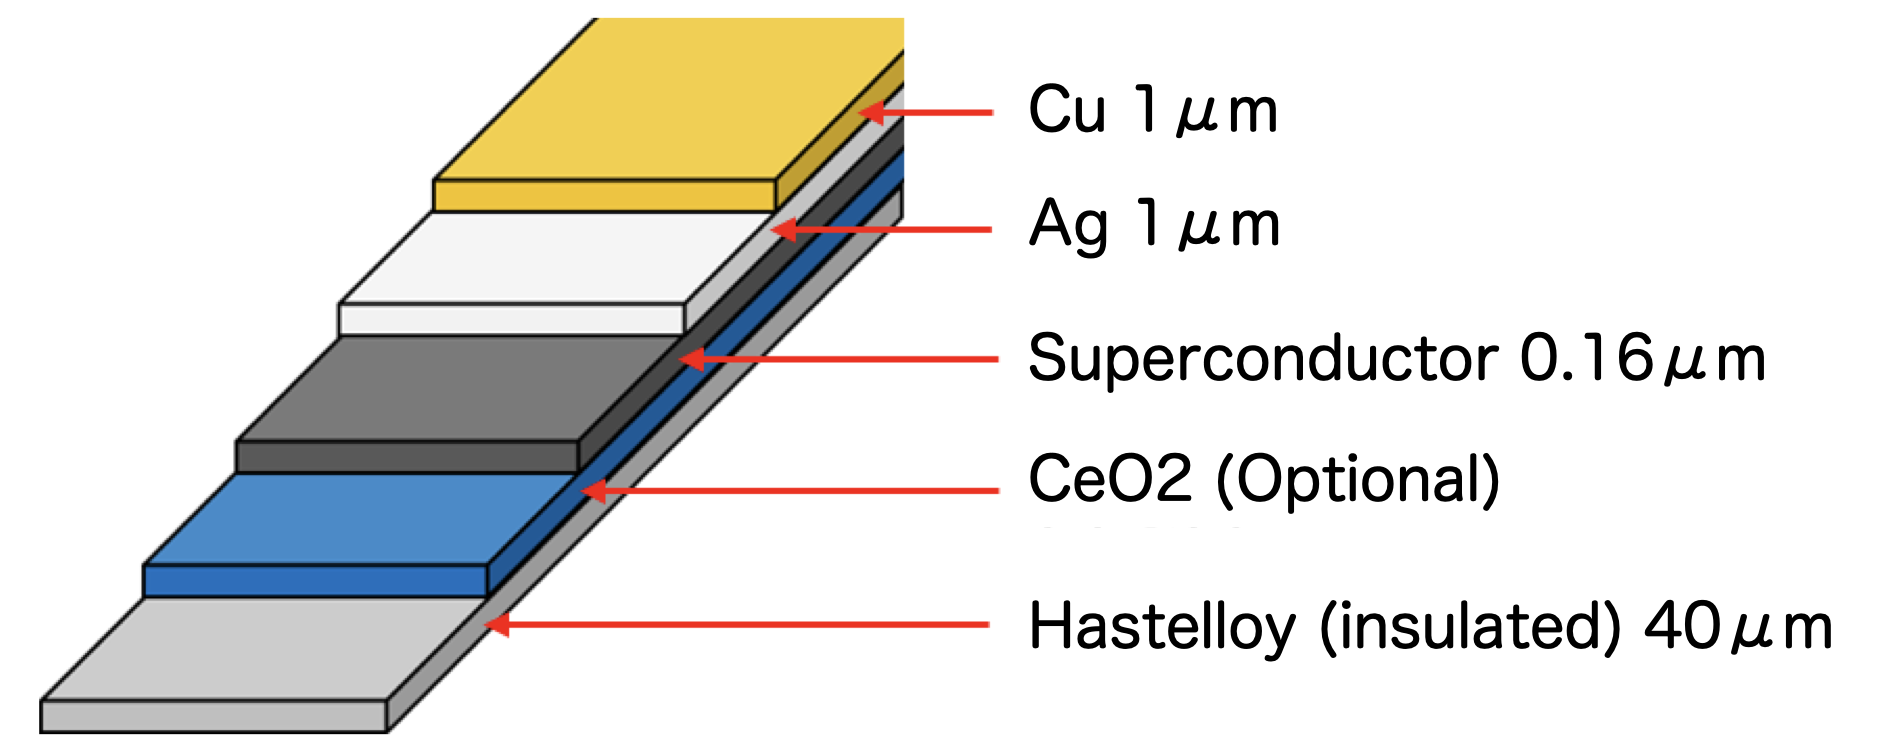
\includegraphics[width=18.5cm, bb=9 9 900 360]{./section2Proposal/Y.png}
  \caption{The layers of a conventional high temperature superconductor tape.}
  \label{fig:Y}
\end{figure}
\begin{table}[H]
  \centering
  \caption{Shielding effects under various magnet thickness(a/b) and relative permeability($\mu_r$).}
  \label{tab:Y}
  \begin{tabular}{cc|rrrrr}\hline\hline
    a/b &  & 0.99 & 0.8 & 0.6 & 0.4 & 0.2\\\hline
    $H_{internal}/H_{external}$ & $\mu_r = 100$ & 3/5 & 1/12 & 1/18 & 1/22 & 1/23 \\
    $H_{internal}/H_{external}$ & $\mu_r = 1000$ & 3/23 & 1/109 & 1/175 & 1/209 & 1/221 \\\hline\hline
  \end{tabular}
\end{table}

The question why many materials show the mysterious behavior of superconductivity remains open, although a part of it is considered solved.
In 1948 Fritz London proposed that the phenomanen may be consequences of the coherence of a quantum state \cite{2_10}.
With further studies, a widely accepted explanation has been published by J. Bardeen, L. Cooper and J. R. Schrieffer in 1957, called the BCS theory \cite{2_11}.
Generally, it was considered impossible for electrons to move without resistance above strict 0 K since the atom vibration was assumed unavoidable from a thermodynamic perspective.
To reach the state of superconductivity, some attractive forces must have worked to condensate electrons into groups which have the state of minimum energy.
However, since the electron is a fermion, the Pauli exclusion principle and the Coulomb repulsion must be overcame before it can be condensated.
The BCS theory assume that electrons attracted each others by exchanging the phonon, and consequently bound together in Copper pair forms in which the state has a lower energy than the Fermi energy.
This minimum energy state achieved by Copper pair origined from the electron-phonon interaction is believed to be the cause of the conventional superconductivity.
While this theory can explained most of the superconductor found before 1980s, namely the first kind superconductor or the low temperature superconductor,
it fails to give a full derivation on the modern high temperature superconductor.

For the HTS, the formation of Copper pair is considered to be somehow participated in the mechanism, but agreement on the reason hasn't been reached.
A relatively new theory has been published in 2016 \cite{2_12}, claiming that an unexplained behavior of the electrons in HTS,
which might be the direct origin of superconductor, has been observed in computer simulation.
Denoting the full detail of the mechanism in superconductivity is beyond the scope of this thesis,
but the phenomanen can be realised in a macroscopic perspective from which the perfect conductivity can be achieved and the notable Meissner effect should be marked.
A well written macroscopic introduction of superconductivity by Fritz London is available in his book \cite{2_10}.


\newpage
\subsection{Ferromagnetism}
\subsubsection{Sense of Magnetism}
Before the ferromagnetism is discussed, we would like to introduce some important properties of magnetism which even undergraduated students majored in electrical engineering might not have learned deeply.
To know the fundamental of a magnetic field, first we tried to measure the magnetic force among various materials.
Consider a huge coil which generates a 3 T field in the central point, like Fig. \ref{fig:2_coil}.
\begin{figure}[H]
  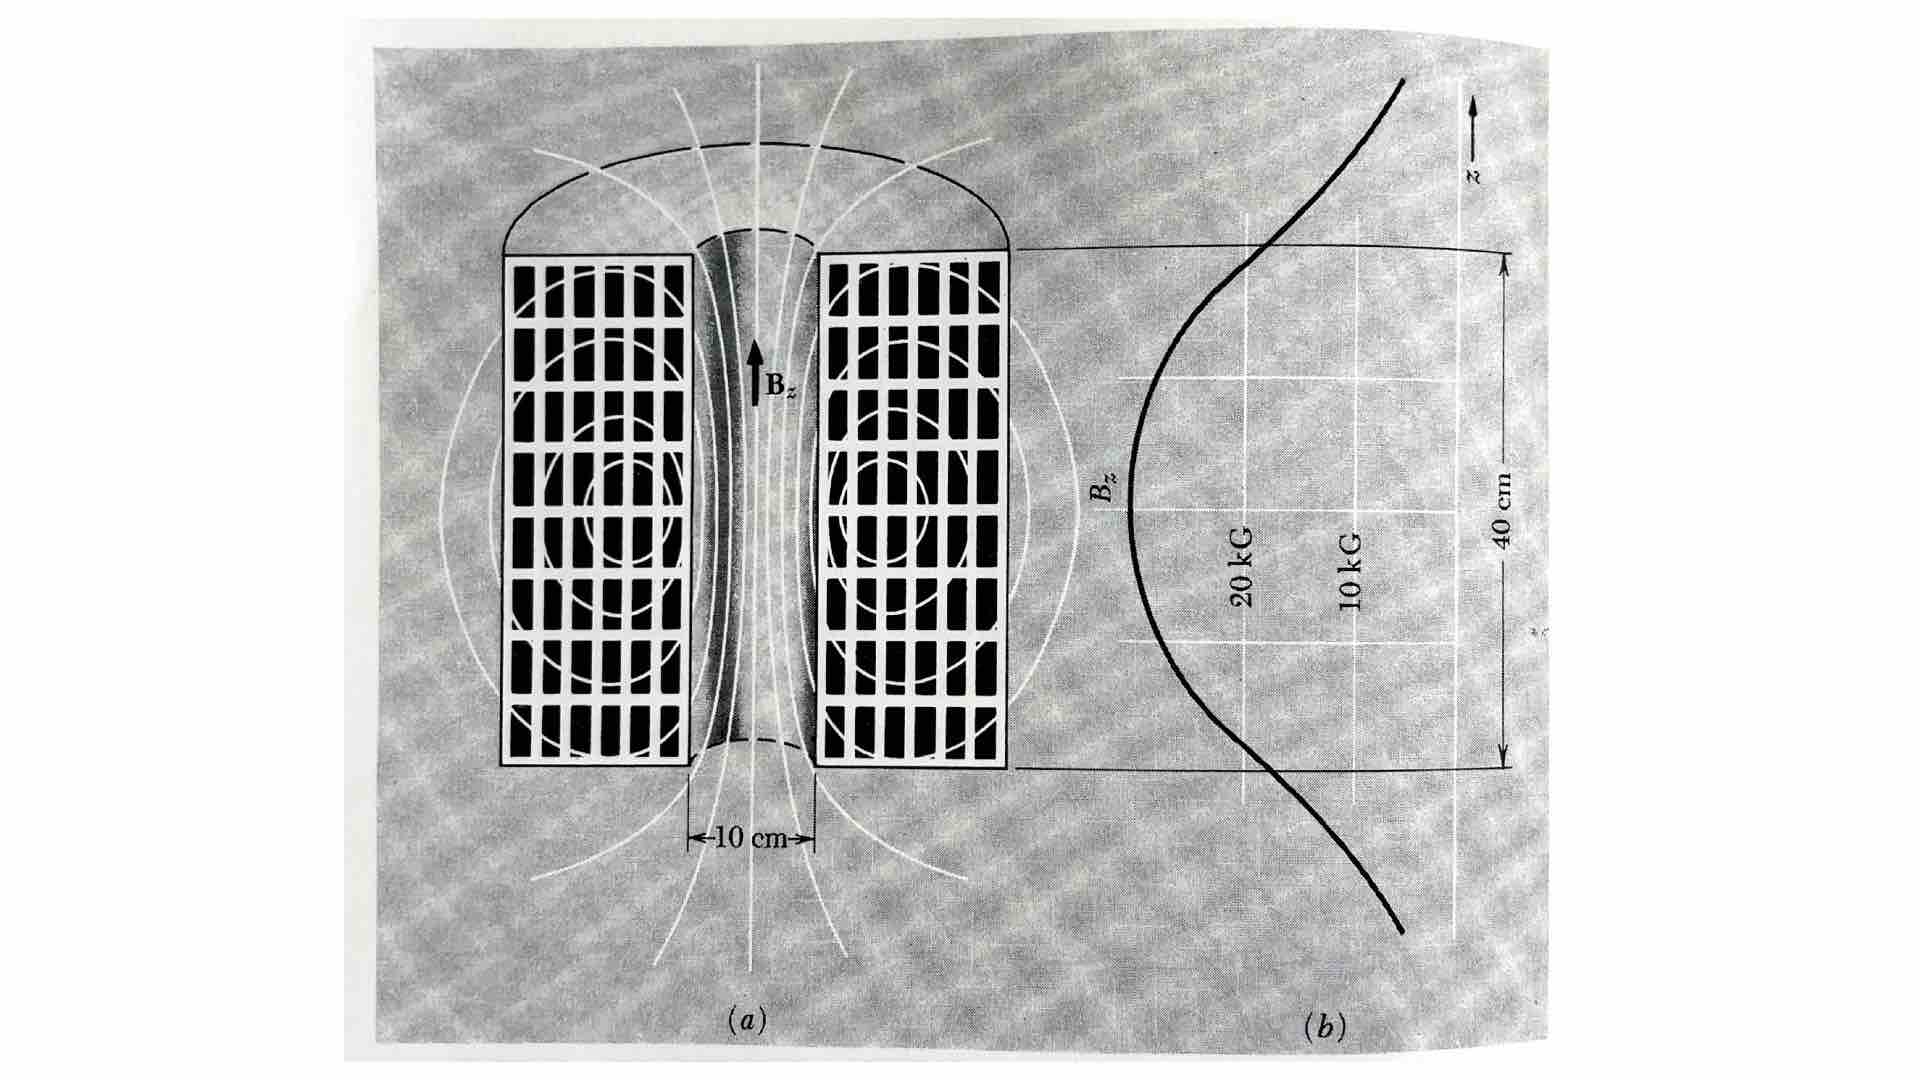
\includegraphics[width=18.5cm, bb=9 9 900 500]{./section2Proposal/3TCoil.JPEG}
  \caption{Schematic drawing of a conventional coil.\cite{2_13}}
  \label{fig:2_coil}
\end{figure}
The field is $10^5$ times of the geomagnetism, and is approximately 10 times more than the field near a common magnet.
From which, we know that the coil used in our experiment is a relatively large scale but not completely unrealistic one at all.
If we measured the force exerted on different materials when they are put along the central axis of the coil,
we would get some interesting results:
\begin{table}[H]
  \centering
  \caption{Force recieved in the electric coil among different materials.\cite{2_13}}
  \label{tab:2_coilResult}
  \begin{tabular}{cr}\hline\hline
    Material & Force [mN] (positive for attraction) \\\hline
    Diamagnetic & \\
    $\mathrm{H_2O}$ & $-2.2$\\
    Cu & $-0.26$\\
    NaCl & $-1.5$\\
    S & $-1.6$\\
    C (graphite) & $-1.6$\\
    C (diamond) & $-11.0$\\
    $\mathrm{N_2}$ (liquid@78 K) & $-1.0$\\\hline
    Paramagnetic & \\
    Na & $+2.0$\\
    Al & $+1.7$\\
    $\mathrm{CuCl_2}$ & $+28.0$\\
    $\mathrm{NiSO_4}$ & $+83.0$\\
    $\mathrm{O_2}$ (liquid@90 K) & $+750.0$\\\hline
    Ferromagnetic & \\
    Fe & $+40,000$\\
    $\mathrm{Fe_3O_4}$ & $+12,000$\\\hline
  \end{tabular}
\end{table}
\begin{enumerate}
  \item The maximum force occured not at the central point, but where the $dB_z/dz$ maximized, namely at the edge of the coil.
  \item The exerted force is related rather to the weight than to the shape of the sample .
  \item Despite the powerful field we have prepared, for most of the samples, the force measured is way too small.
  For typical values, $0.1\sim0.2$ N/kg are measured, which is no greater than a few percentage of their weights.
  \item When the imposed field is increased continueously, some samples tend to be attracted while the others are repulsed.
  This completely opposite behavior against magnetic force among the samples are extraordinary,
  and immediately indicates that the common materials on Earth can be devided into 2 groups,
  one attracted by the magnetic field, the other being repulsed.
  \item Within the samples, we have discovered a few of them showing strong attraction from the field.
  For example, the crystal of $\mathrm{CuCl_2}$ is attracted by $2.8$ N/kg down into the central.
  Liquid oxygen has shown an attraction of $75$ N/kg, about 8 times larger than its weight.
  On contrast, liquid nitrogen only showed a weak repulsion of $10^{-4}$ N/kg.
  The same trend occured on copper and iron, among which a huge difference of $10^5$ N in magnitude is observed.
  The total result is stated in Tab. \ref{tab:2_coilResult}.
  \item Whether the force changed proportionally to the imposed field has also shown an obvious difference between the samples.
  When the imposed field was cut in a half,
  forces measured on the materials listed before iron in Tab. \ref{tab:2_coilResult} descreased to $1/4$,
  while the others only dropped to about $1/2$ or even higher.
\end{enumerate}

From the above, obviously, the phenomanen we are facing is complicated.
For the first step to understand magnetism, some classification should be introduced.
Materials showing weak repulsion on magnetic fields are called "diamagnetic",
which most of the materials on Earth are listed in, except for a few inorganic compounds \cite{2_13}.
Diamagnetism is considered a consequence of the general electromagnetic induction from the electron.
Consider a ring made of conductive ingredients.
If it is pushed towards a magnetic field penetraing the cross section, electrical current would be induced,
generating an opposite field to push itself outside the field.
This phenomanen, often known as the Lentz's law,
is similar to what has happened in the experiment when we tried to push a material into some magnetic field.
Since every atom contains electrons, diamagnetism is the general behavior when a certain material interacts with the magnetic field.

When attraction on magnetic fields is observed,
it indicates that some other effects more dominant than the diamagnetism must have been participated in.


\newpage
\subsubsection{Modern Ferromagnetic Materials}
Conventional ferromagnets list up ferite, cobalt etc. which hold a relative permeability of 1000-10000 and a maximum magnetization of about 700 mT.
Recent researches have reached a magnetization as high as 1-2 T, using stainless steel and permalloy (a nickel–iron alloy).
The list is shown in Fig. \ref{fig:magnetMaterials}
\begin{figure}[H]
  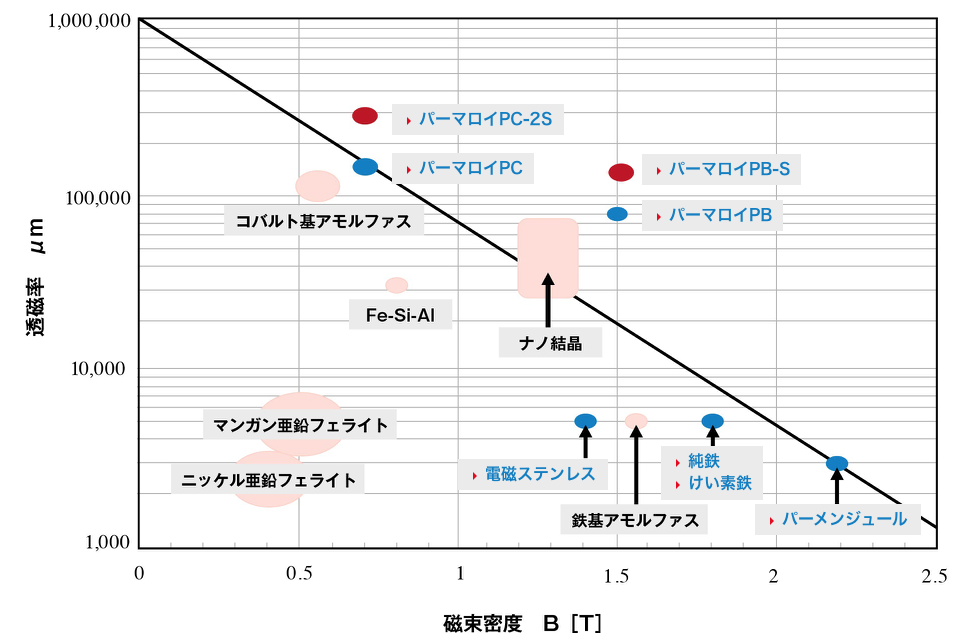
\includegraphics[width=18cm, bb=9 9 900 600]{./section2Proposal/magnetMaterials.png}
  \caption{The conventional and modern ferromagnet materials.}
  \label{fig:magnetMaterials}
\end{figure}
In our research, we have focused on ferite which is a non-oriented ferromagnet with relatively lower maximum magnetization to satisfy our request of simulating a situation in which magnets would go saturated.


\newpage
\subsubsection{Significant but not Apparent Difference among the ${\bm B}$ Field, ${\bm H}$ Field and ${\bm M}$ Field}
In applied electrical engineering, the field $H$ and field $B$ are often seen having the same direction.
This is true in the case that magnetization is not participated in,
while near a strong magnet the magnetization enrolls,
leaving the familiar equation
\begin{equation}
  \mathbf{B} = \mu_0\left( \mathbf{H} + \mathbf{M} \right)\nonumber
\end{equation}

To make it clear, a schematic drawing of the surrounding $B$ and $H$ fields near a magnet is shown in Fig. \ref{fig:BandH}.
\begin{figure}[H]
  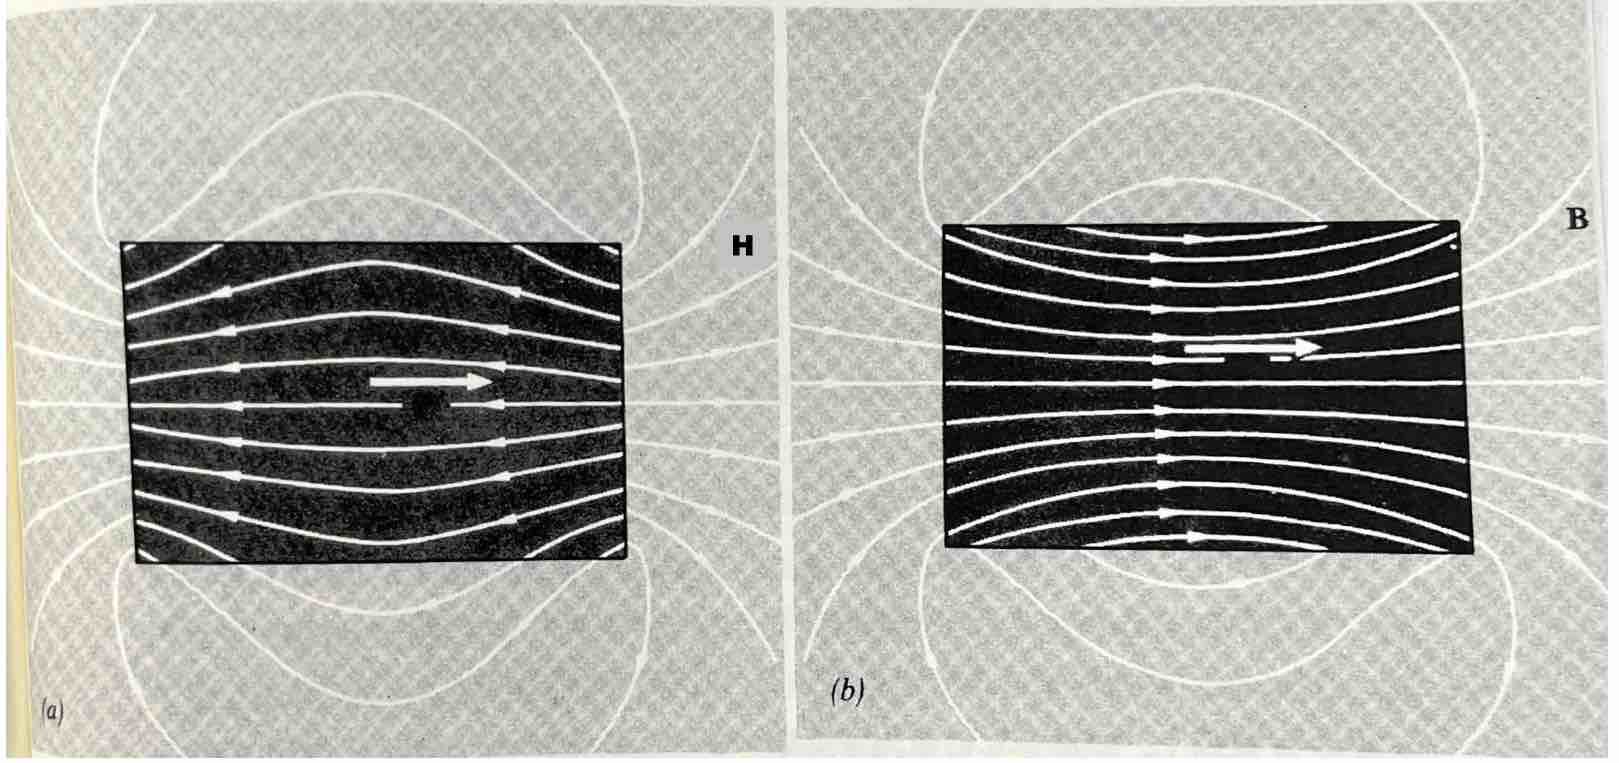
\includegraphics[width=18cm, bb=9 9 900 550]{./section2Proposal/BandH.JPEG}
  \caption{The (left) $H$ field and (right) $B$ field near a conventional magnet.}
  \label{fig:BandH}
\end{figure}
In Fig. \ref{fig:BandH}, it is appearant that both fields on the outside of the magnet distributed identically strictly,
while on the inside part the are totally different with approximately opposite direction.
In fact, the $H$ field is strictly the same as the $E$ field under the condition that the magnet is substituded by a conventional capacitor where opposite irons gathering around the 2 poles.
This indicates that $H$ field can be seen as origining from a scalar potential,
with virtual plus magnetic monopole gathering on the left pole of the magnet,
and minus magnetic monopole gathering on the right pole of it.

The different distribution between the internal $H$ and $B$ field results from the fact that
the $B$ field origins from a vector potential,
or in other terms,
satisfies the equation.
\begin{equation}
  div\mathbf{B} = 0\nonumber
\end{equation}
This equation describes the $B$ field must be continueous anywhere,
generating a near field shown in Fig. \ref{fig:BandH}.

Now, the magnetization term $M$ comes in to fullfill the equation
\begin{equation}
  \mathbf{B} = \mu_0\left( \mathbf{H} + \mathbf{M} \right)\nonumber
\end{equation}
In a magnet, strong $M$ would be exited along the $B$ field to cancel out the $H$ field.
A scematic drawing of this concept is shown in Fig. \ref{fig:BandHandM}.
\begin{figure}[H]
  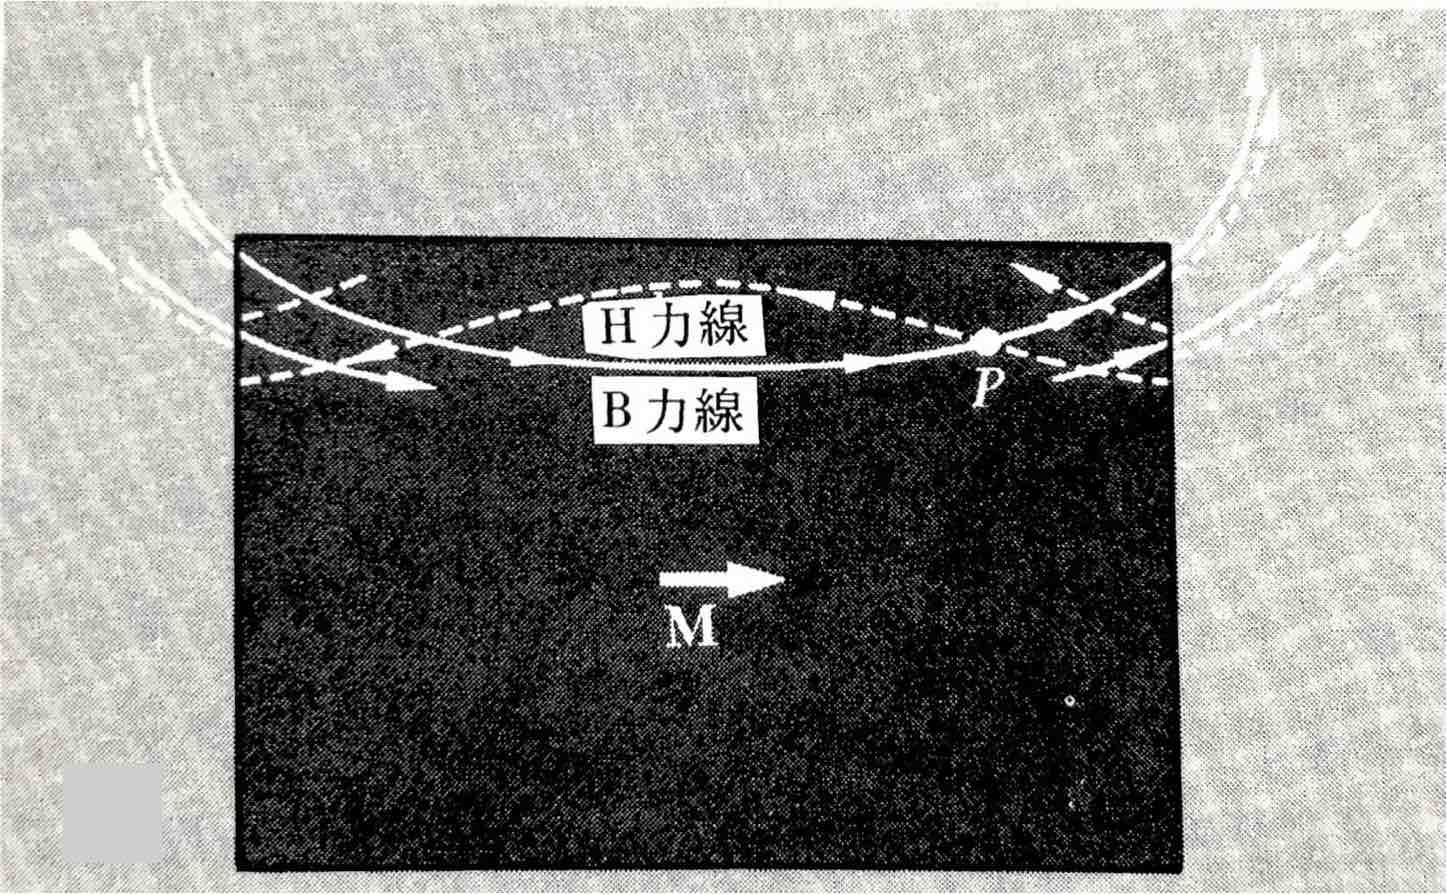
\includegraphics[width=18cm, bb=9 9 900 550]{./section2Proposal/BandHandM.JPEG}
  \caption{The $H$ and $B$ and $M$ field near a conventional magnet.}
  \label{fig:BandHandM}
\end{figure}


\newpage
\subsection{Conventional Magnetic Cloak}
A magnetic cloak using low temperature superconductor bulks and ferromagnets is first published in Fedor's work \cite{2_20}.
The key idea is to combine superconductor bulk with ferromagnet to achieve the cloaking ability,
of which the schematic drawing has been already shown in Fig. \ref{fig:cloak}.
To describe the cloak of magnetic field, the field along certain tangent line on the surface is shown in Fig. \ref{fig:cloakSurfaceLine}.
\begin{figure}[H]
  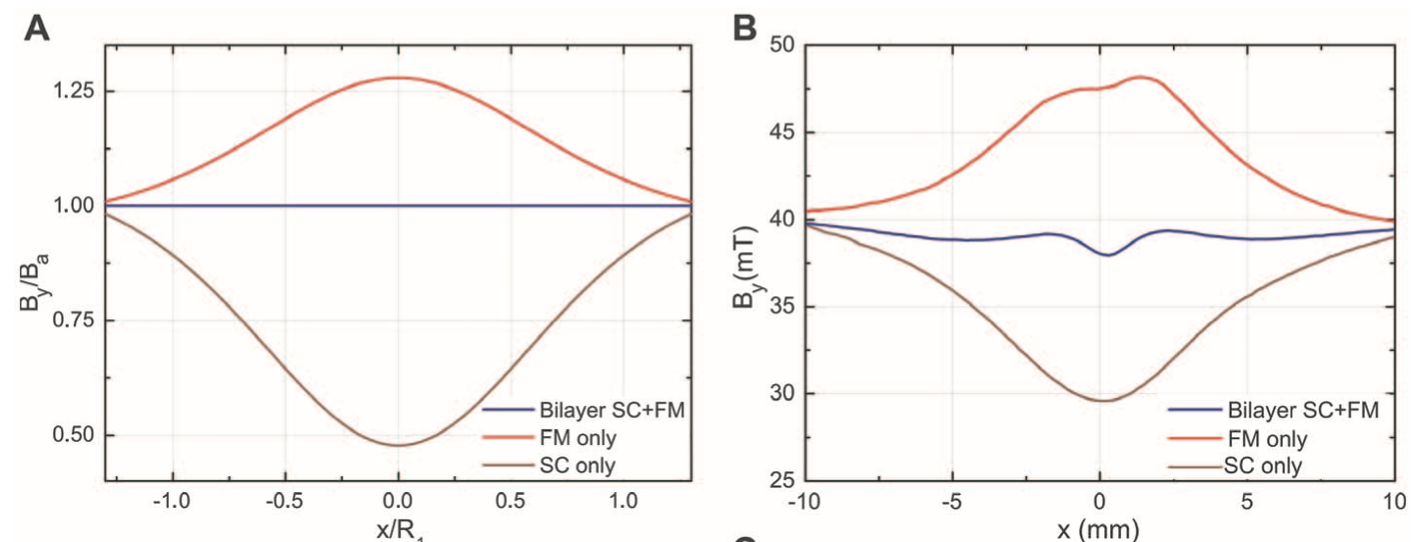
\includegraphics[width=17cm, bb=9 9 900 550]{./section2Proposal/cloakSurfaceLine.png}
  \caption{The magnetic field along the top line. (A) calculation; (B) experimental.\cite{2_20}}
  \label{fig:cloakSurfaceLine}
\end{figure}
From Fig. \ref{fig:cloakSurfaceLine}, it is obvious that nearly perfect cloaking ability can be achieved.
In other words, by adapting the Meissner effect of superconductor and the magnetization phenomenen of ferromagnet,
shielding outer field while not disturbing it is possible.
However, the Meissner effect can only tolerate a few tens of 10 mT, which in turn makes the conventional magnetic cloak impossible to work under high fields.


\subsection{Electromagnetic-Induction Type Magnetic Cloak}
To overcome this problem and develope a magnetic cloak like equipment suit for operation under high fields of a few Tesla,
we have proposed a brand new magnetic cloak named the "Electromagnetic Induction Type Magnetic Cloak",
which applys the perfect conductivity property instead of the Meissner effect.
The main structure is shown in Fig. \ref{fig:EIMCStructure}.
\begin{figure}[H]
  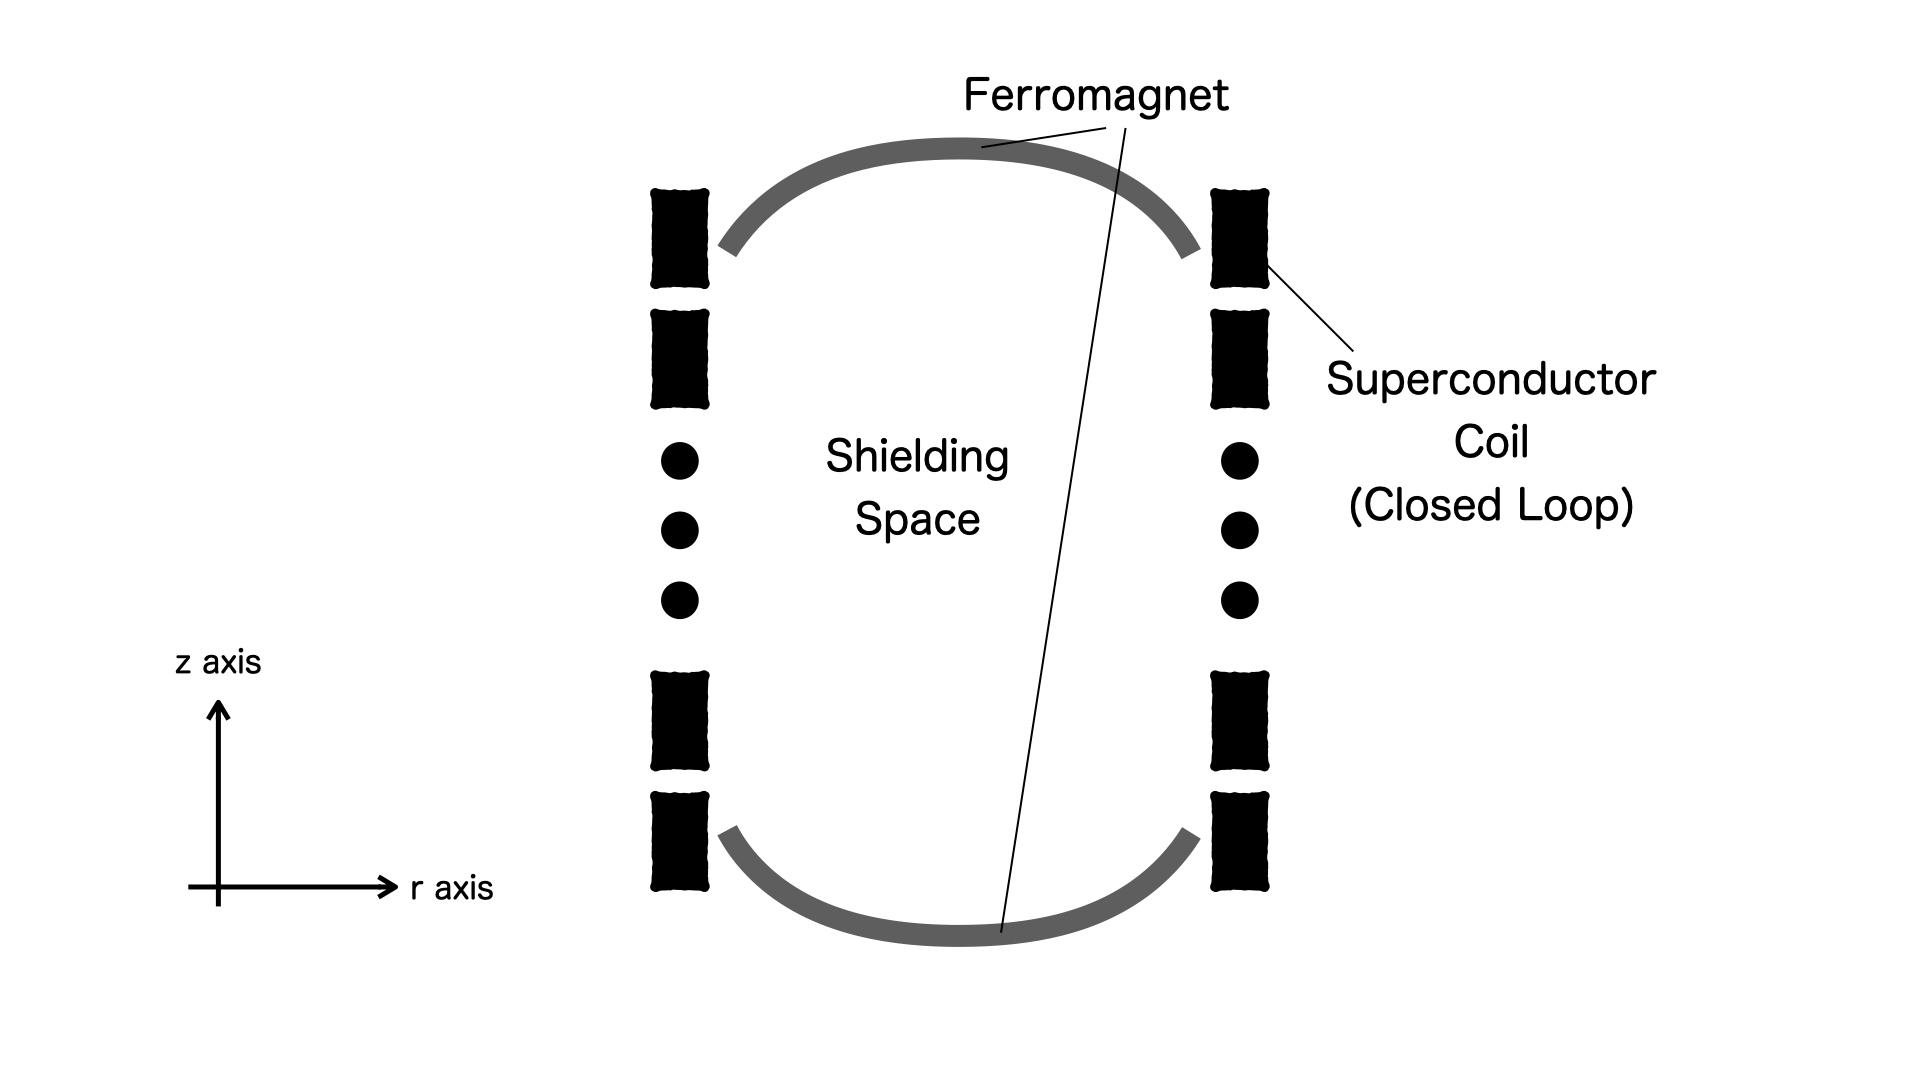
\includegraphics[width=13cm, bb=9 9 900 550]{./section2Proposal/EMICStructure.png}
  \caption{The structure of Electromagnetic Induction Type Magnetic Cloak.}
  \label{fig:EIMCStructure}
\end{figure}
First we connect the superconductor windings to make a huge closed loop.
Then, ferromagnets are placed on the top and the bottom edge of the coil.
The following procedure shows how it works.
\begin{figure}[H]
  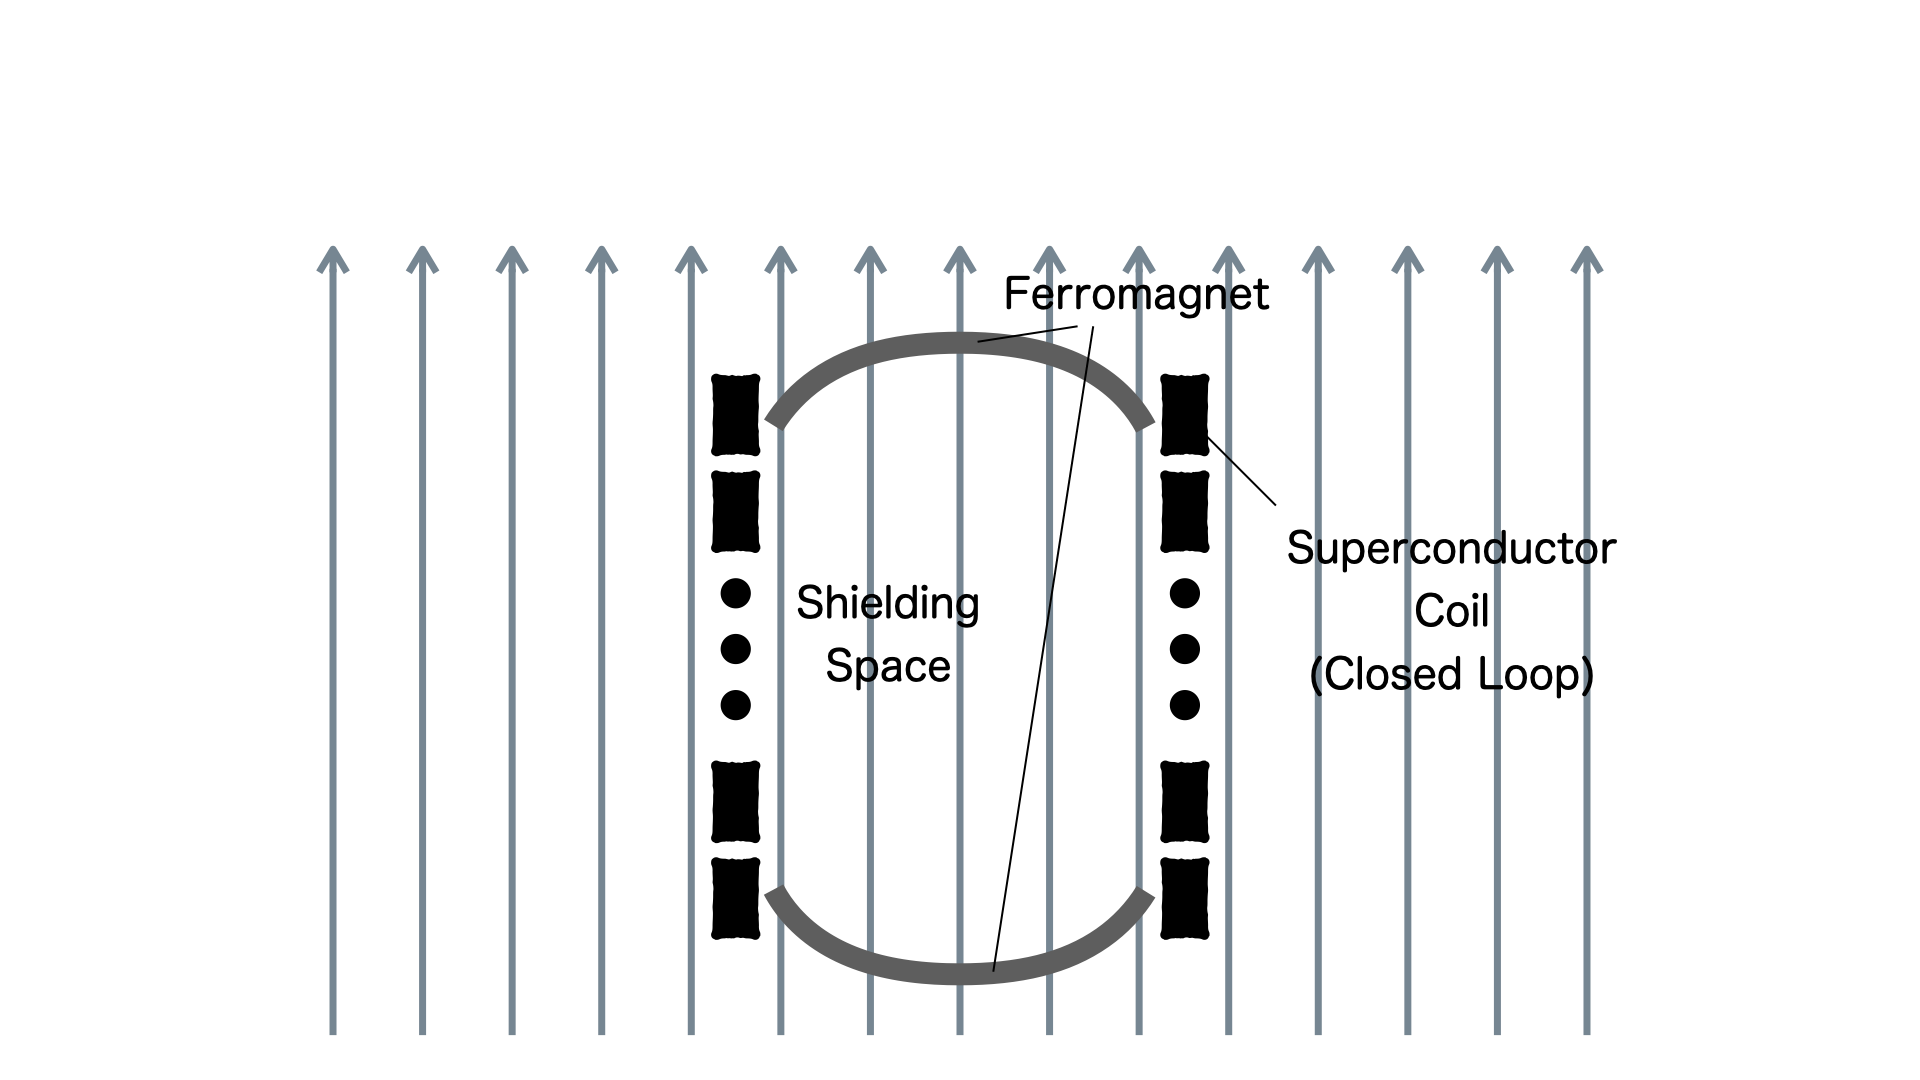
\includegraphics[width=13cm, bb=9 9 900 550]{./section2Proposal/EMIC1.png}
  \caption{Solenoid superconductor windings imposed by external field (before).}
  \label{fig:EIMC1}
\end{figure}
\begin{figure}[H]
  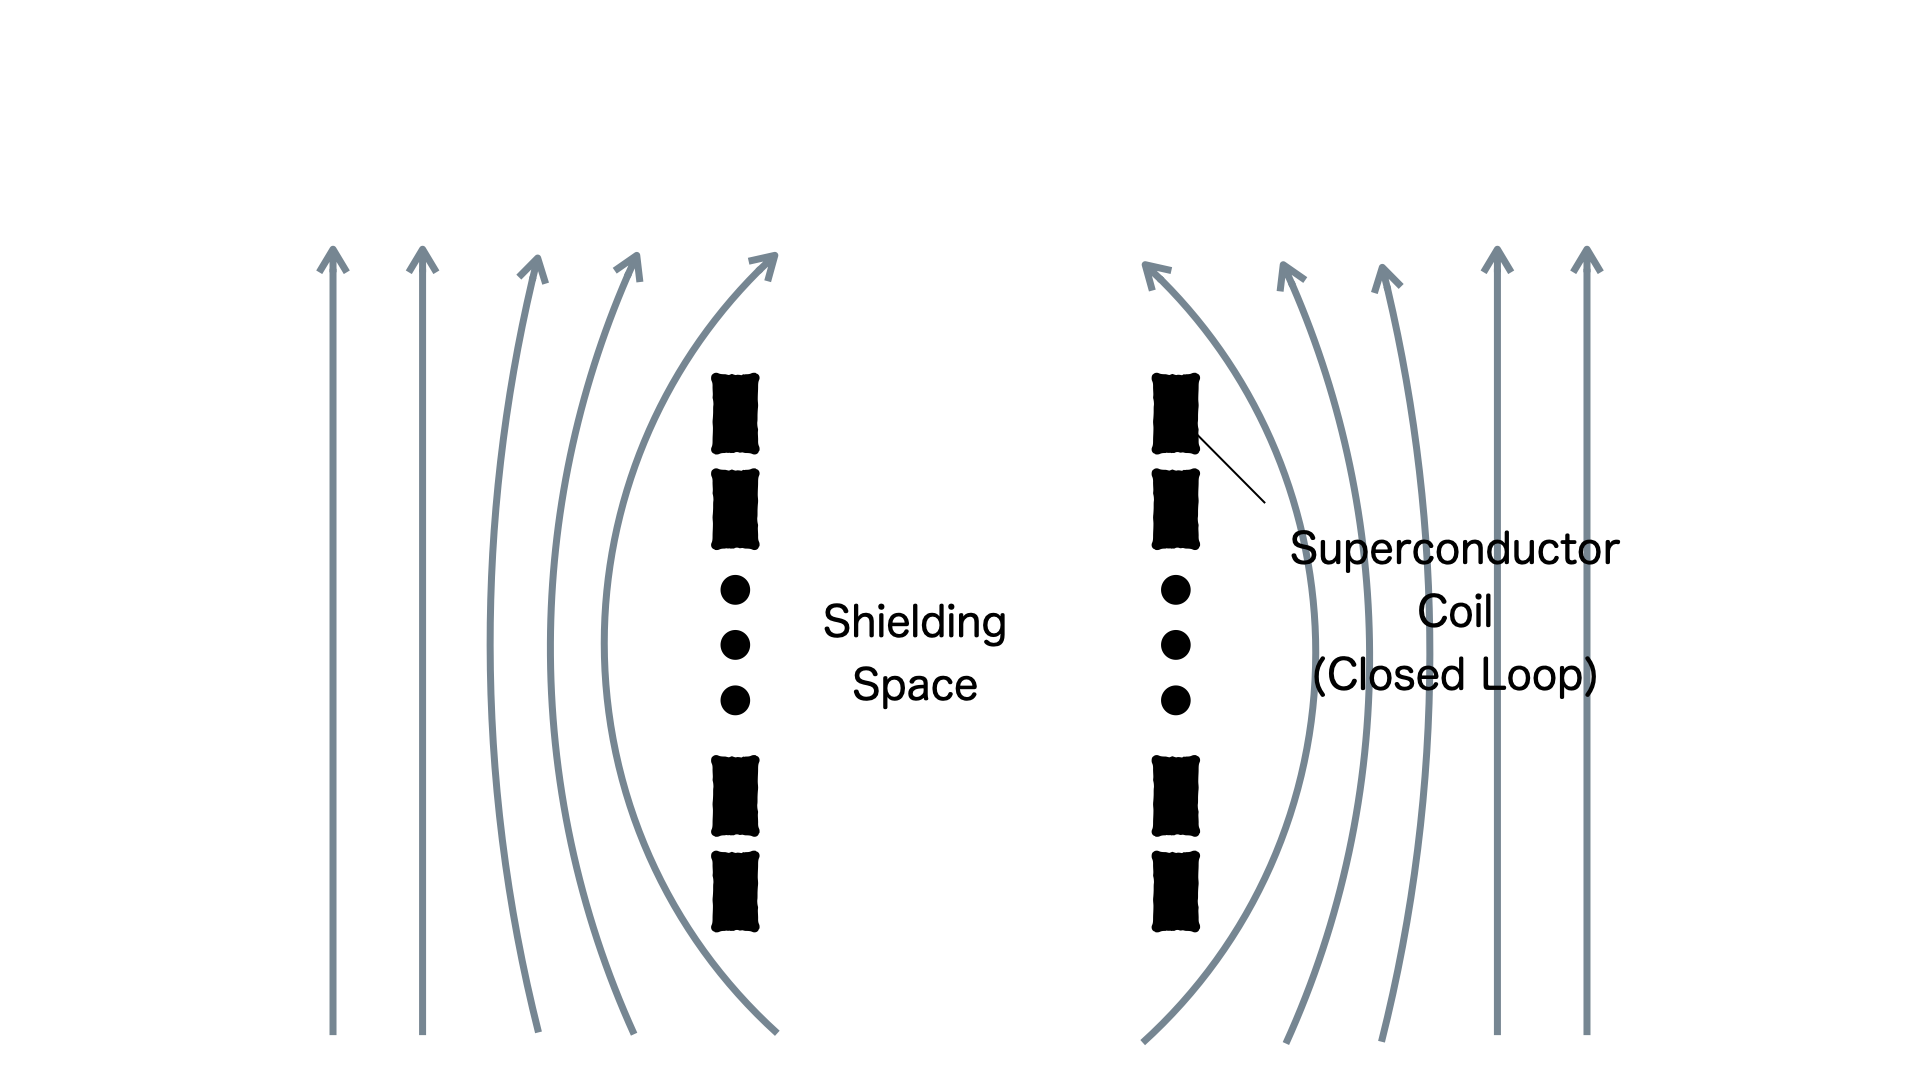
\includegraphics[width=13cm, bb=9 9 900 550]{./section2Proposal/EMIC2.png}
  \caption{Solenoid superconductor windings imposed by external field (before).}
  \label{fig:EIMC2}
\end{figure}
\begin{figure}[H]
  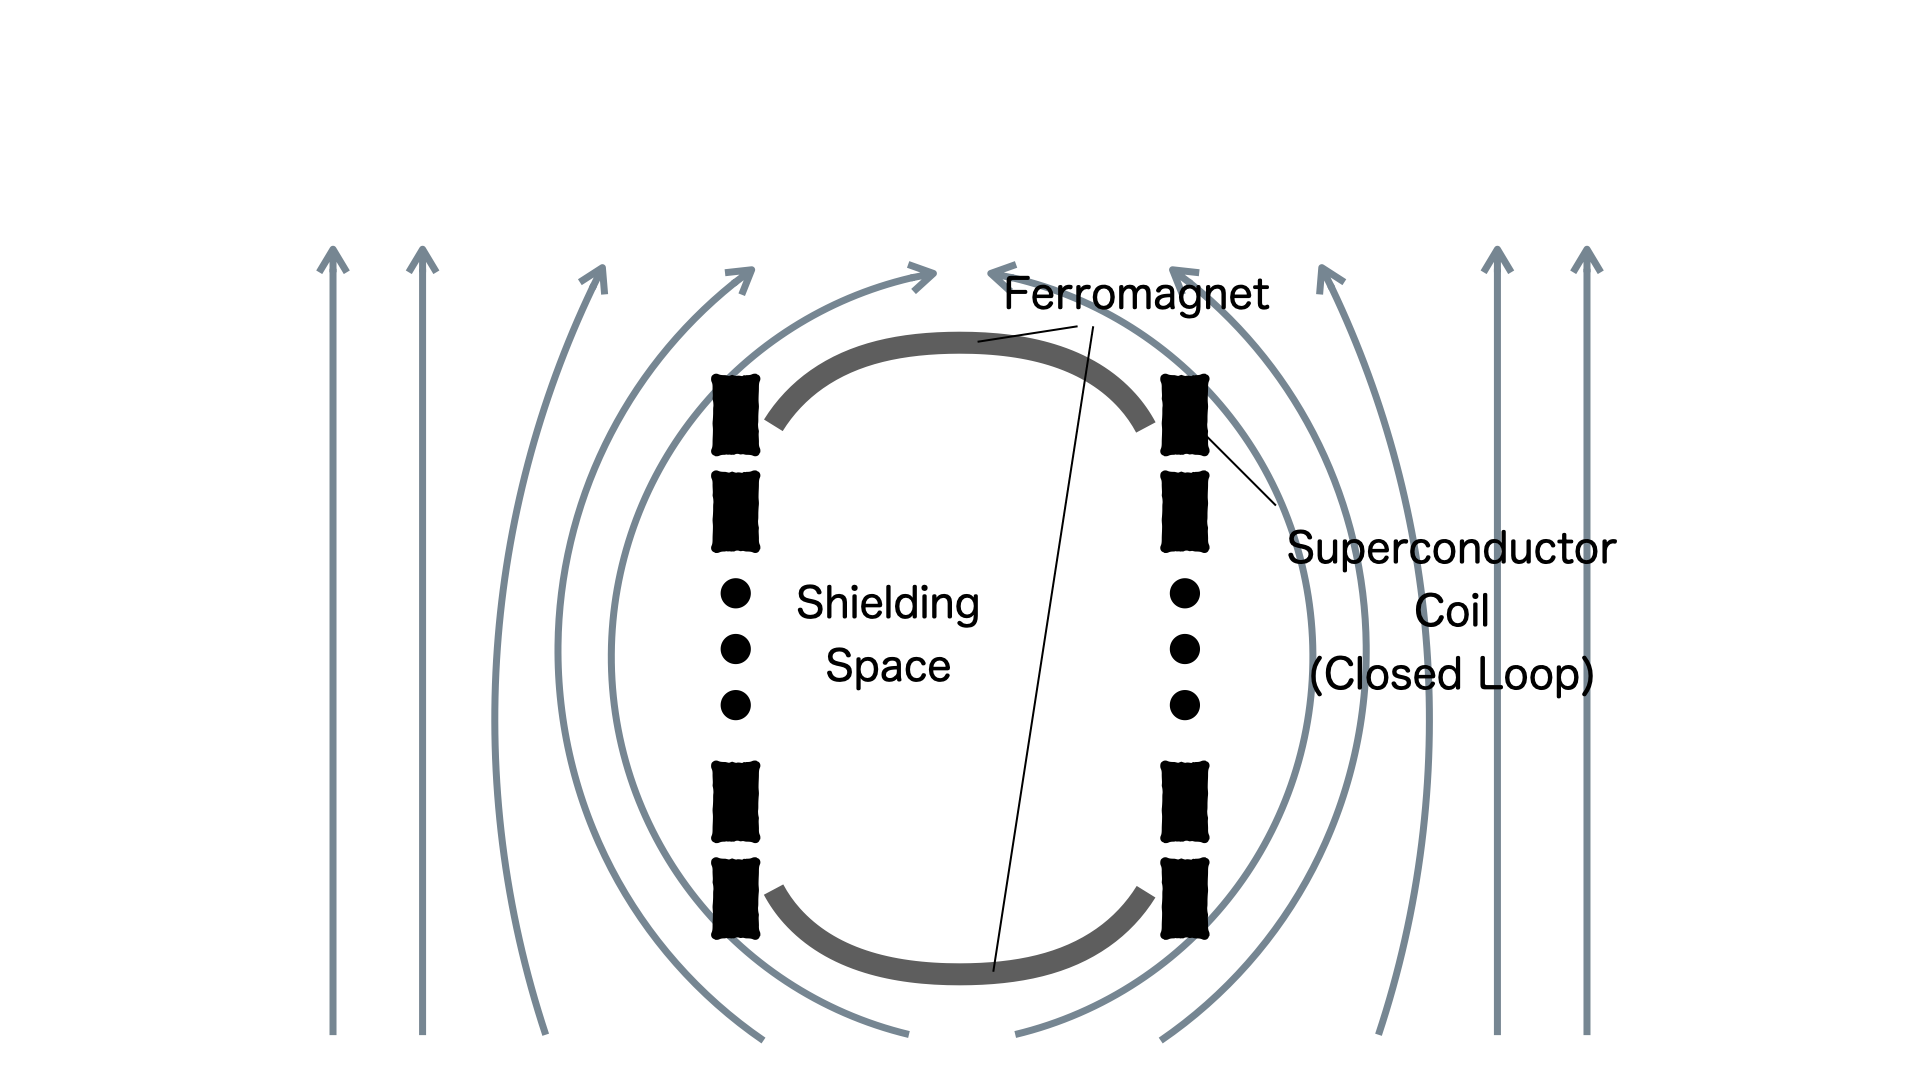
\includegraphics[width=13cm, bb=9 9 900 550]{./section2Proposal/EMIC3.png}
  \caption{Adding ferromagnet on the edge of the coil should reinforce the outer field near the edge.}
  \label{fig:EIMC3}
\end{figure}
If we impose magnetic field from the external,
since the tapes are closed and in the superconducting state,
huge permenant current would be induced,
canceling out the external field (Fig. \ref{fig:EIMC1}$\to$Fig. \ref{fig:EIMC2}).
Moreover, if ferromagnets are placed on the top and bottom edge additionally,
the outer field would be reinforced by the strong magnetization.
Since more turns the superconductor windings is made of,
more canceling field can be generated,
which gives the model full scalability to high fields.
We have named this model "Electromagnetic Induction Type" to distinguish it from the conventional magnetic cloak using Meissner effect.

With this concept, a shielding system with cloaking property capable of working under high field environment can be expected.
In the following chapter, we show the studied effectiveness of it.


\newpage
\begin{thebibliography}{20}
  \bibitem{2_1} Fritz London, "Superfluids I, Macroscopic Theory of Superconductivity" (1950)
  \bibitem{2_2} H. Kamerlingh Onnes, Leiden Comm., 122 b, 124 c (1911)
  \bibitem{2_3} D. B. Cook, M. W. Zemansky, and H. A. Boorse, Phys. Rev. 78, 820 (1950)
  \bibitem{2_4} H. Kamerlingh Onnes and W. Tuyn, Proc. Acad. Sci. Amsterdam, 25, 443 (1923)
  \bibitem{2_5} W. Meissner and R. Ochsenfeld, Naturwissenschaften, 21, 787 (1933)
  \bibitem{2_6} J. G. Bednorz and K. A. Müller, "Possible highTc superconductivity in the Ba−La−Cu−O system", Z. Physik, B 64 (1), p. 189–193 (1986)
  \bibitem{2_7} Pia Jensen Ray. Figure 2.4 in Master's thesis, "Structural investigation of La2–xSrxCuO4+y - Following staging as a function of temperature". Niels Bohr Institute, Faculty of Science, University of Copenhagen. Copenhagen, Denmark. (2015)
  \bibitem{2_8} Drozdov, A. P.; Eremets, M. I.; Troyan, I. A.; Ksenofontov, V.; Shylin, S. I., "Conventional superconductivity at 203 kelvin at high pressures in the sulfur hydride system", Nature. 525 (7567): 73–76. (2015)
  \bibitem{2_9} Snider, Elliot; Dasenbrock-Gammon, Nathan; McBride, Raymond; Debessai, Mathew; Vindana, Hiranya; Vencatasamy, Kevin; Lawler, Keith V.; Salamat, Ashkan; Dias, Ranga P., "Room-temperature superconductivity in a carbonaceous sulfur hydride", Nature. 586 (7829): 373–377 (Oct. 2020)
  \bibitem{2_10} London, F. (September 1948). "On the Problem of the Molecular Theory of Superconductivity", Physical Review. 74 (5): 562–573 (1948)
  \bibitem{2_11} J. Bardeen, L. Cooper and J. R. Schrieffer, "Theory of superconductivity", Phys. Rev. 108 1175 (1957)
  \bibitem{2_12} Shiro Sakai, Marcello Civelli, and Masatoshi Imada, "Hidden Fermionic Excitation Boosting High-Temperature Superconductivity in Cuprates", Phys. Rev. Lett. 116, 057003 (2016)
  \bibitem{2_13} Edward M. Purcell, "バークレー物理学コース 電磁気 復刻版 (Berkeley Physics Course Electricity and Magnetism)" (2013)
  \bibitem{2_20} Fedor Gömöry et al., "Experimental Realization of a Magnetic Cloak", Science 335, 1466 (2012)
\end{thebibliography}


\newpage
\section{Effectiveness of the Electromagnetic-Induction Type Magnetic Cloak}
% section 3 Effectiveness
In this chapter, the attemption to proof the effectiveness of our proposed electromagnetic-induced type magnetic cloak is denoted.
To confirm the ability of shielding high fields, three significant parameters have been investigated:
\begin{enumerate}
  \item Time Constant. Since electrical induction is applied in the proposed cloak,
  a long enough time constant of the induced current should be ensured.
  \item Shielding Ability. Since the magnetic cloak works as a magnetic shielding equipment,
  the shielding ability is the key function to be questioned.
  \item Effect of Ferromagnet. To maintain the external surrounding fields the magnetization of ferromagnets is adapted,
  of which the effect should be testified.
\end{enumerate}
Different series of experiments and numerical simulation have been conducted respectively to measured each parameter,
of which the theory, method and results are shown in each section.
In the following sections,
the measurement of the time constant is first denoted in 3.1,
that of the shielding ability is followed in 3.2,
and the effect of ferromagnets is described in 3.3.

\newpage
\subsection{Ability of Shielding Stable High Magnetic Fields}
\subsubsection{Purpose}
Although the zero resistance high temperature superconductor tapes are used in EIMC,
electrical resistance still exists at the connected part.
Due to the resistance, the induced current in the superconductor tapes decreased with time.
The descreasing speed of the current in an RC circuit is known to be related to a parameter called the Time Constant.
If the time constant of a coil is large, longer time is required for the current flowing through to change in magnitude.
It can be considered similar to the law of inertia in motion,
in which an object with a large momentum tends to maitain its speed and direction.

When EIMC are used to shield stable fields,
a large time constant should be ensured to allow the induced current and the shielded state stay for long.
The purpose of this section is to confirm this property being large enough from a series of experiments.

\subsubsection{Theory}
To simulate a magnetic cloak working as a magnetic field shielding equipment,
we have conducted an experiment of which the schmetic design is shown in Fig. \ref{fig:experiment}.

To simulate a stable magnetic field, a trapezoid current is imposed on the outer coil,
as shown in Fig. \ref{fig:imposedCurrentExample}.
Additionally, Fig. \ref{fig:DCTimeSeriesExample} shows an example of the measured magnetic field $B_z$ at certain point inside the inner coil.
In which, following the Faraday's law
altering the external field yields current induction on the opposite direction,
which cancels out the imposed field.
\begin{figure}[H]
  \includegraphics[width=17cm, bb=9 9 900 550]{./section3Effectiveness/imposedCurrentExample.png}
  \caption{A example of the imposed trapezoid current.}
  \label{fig:imposedCurrentExample}
\end{figure}
\begin{figure}[H]
  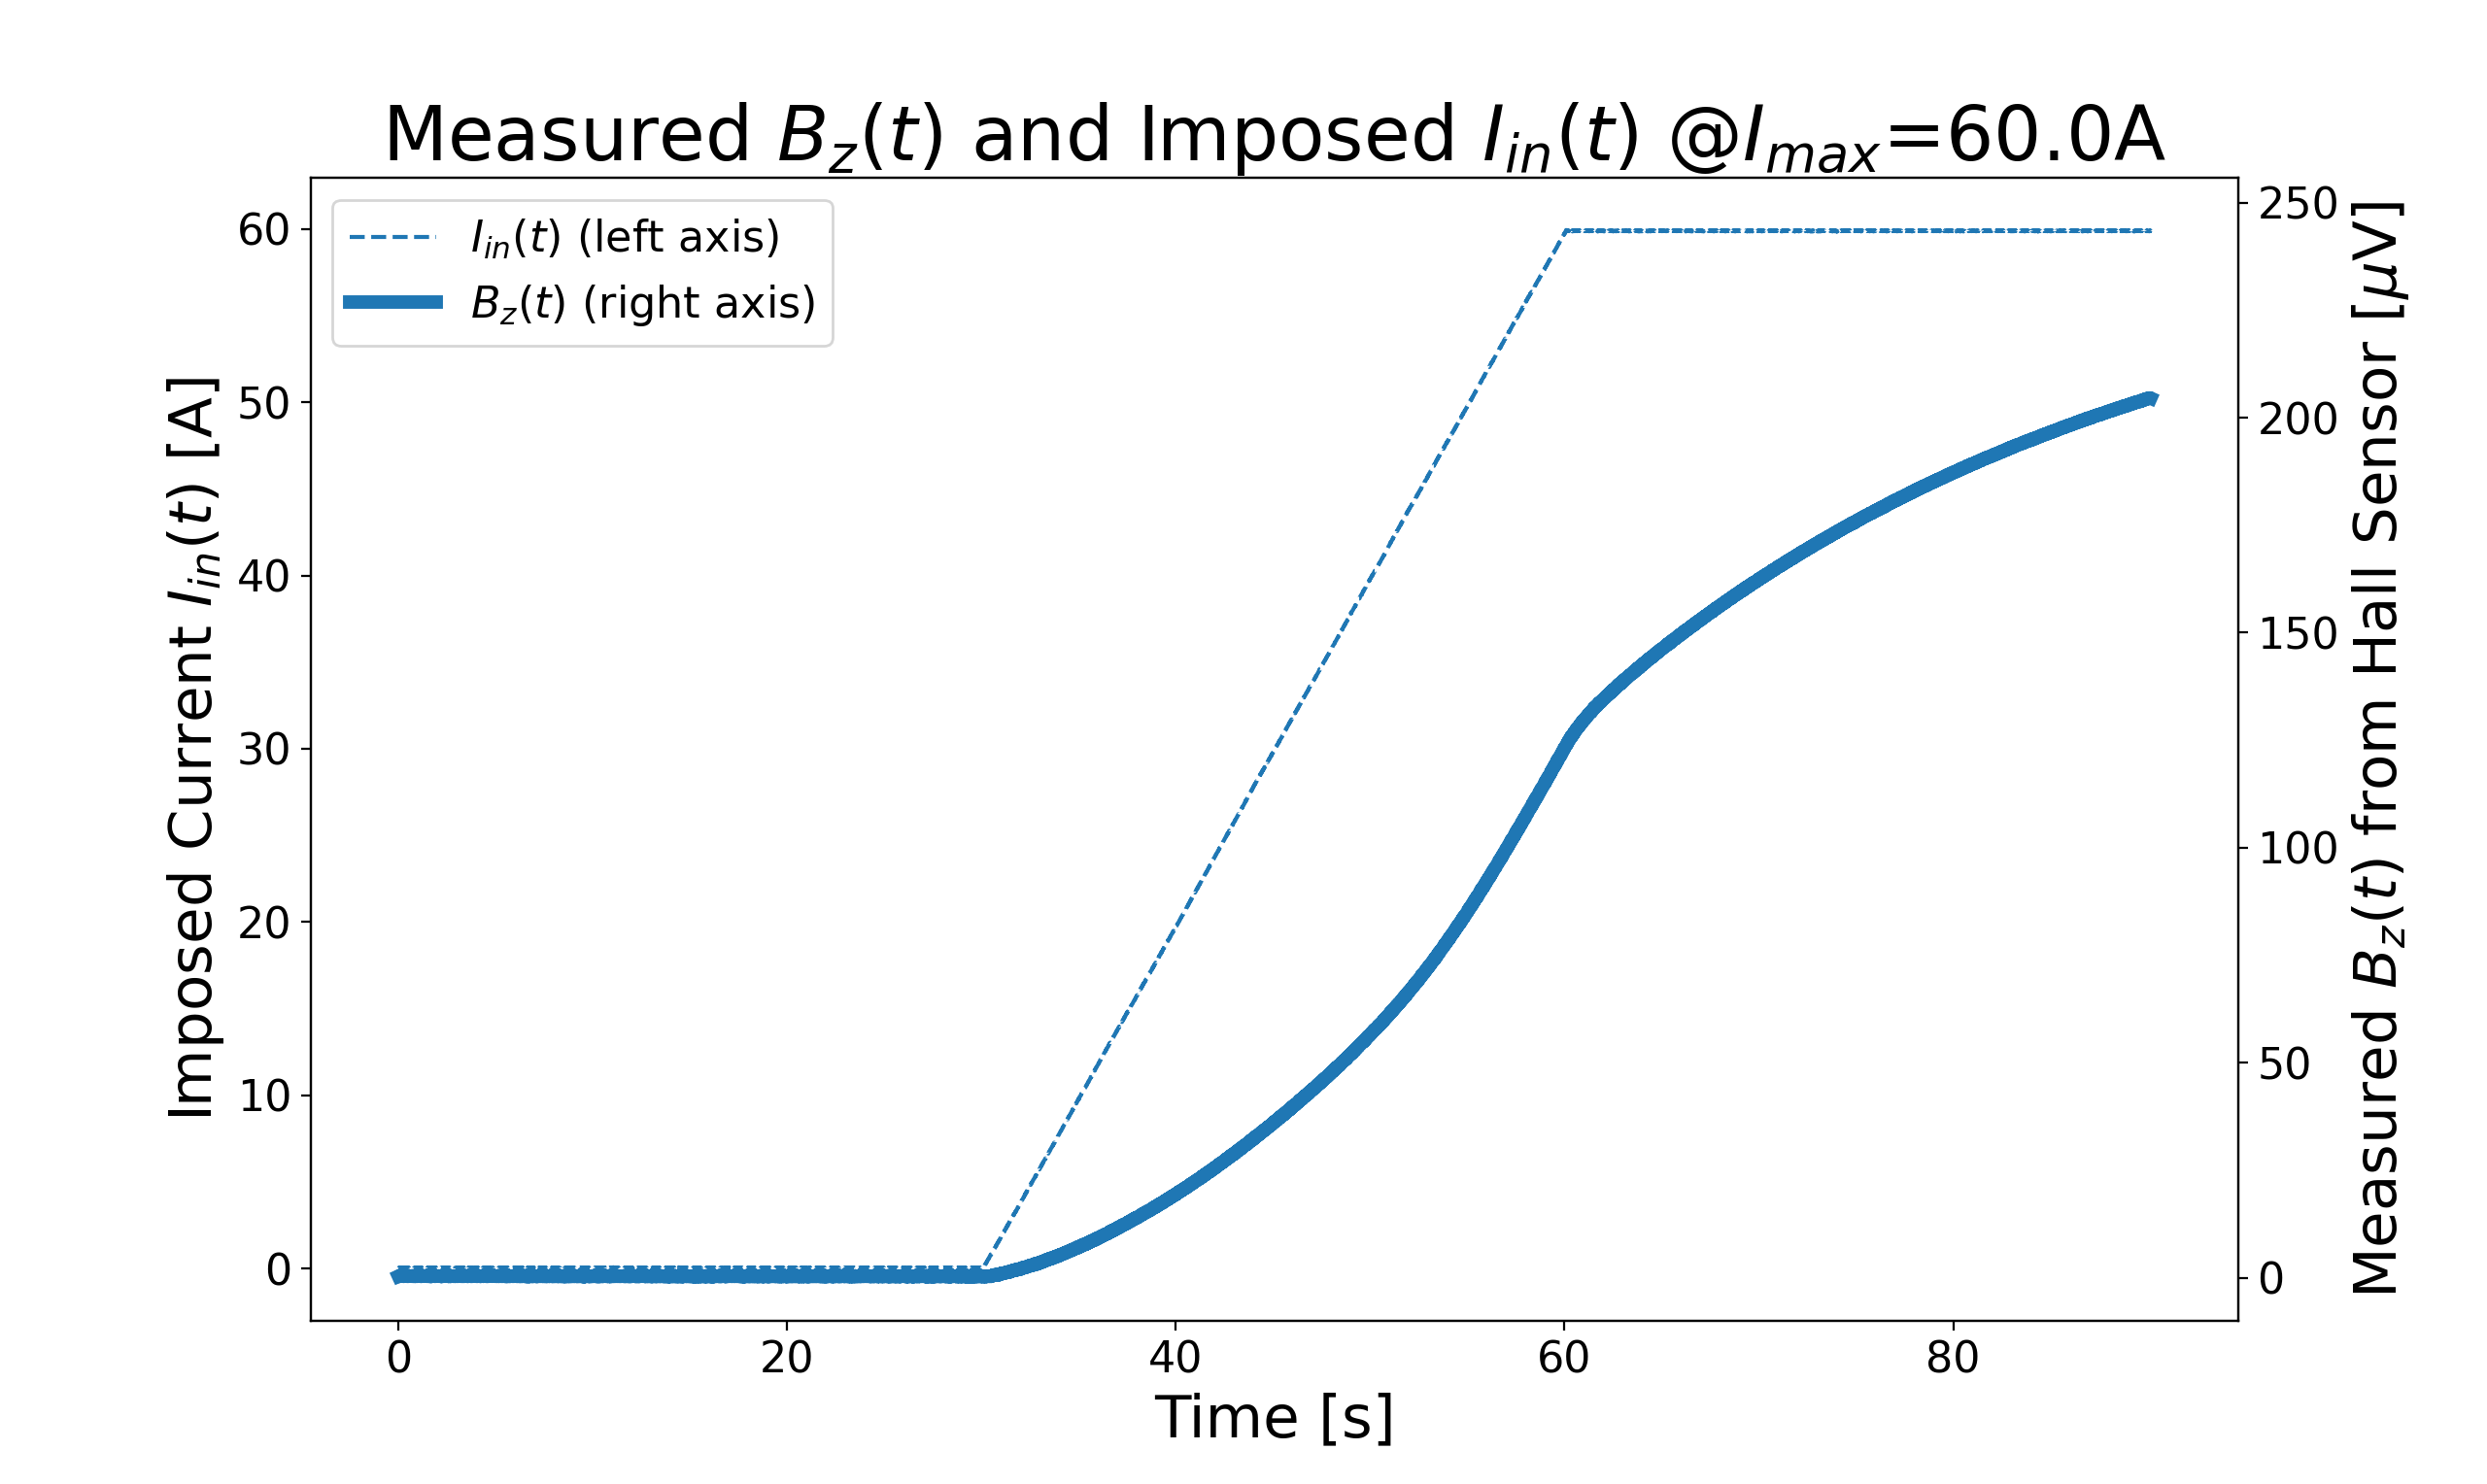
\includegraphics[width=17cm, bb=9 9 900 490]{./section3Effectiveness/DCTimeSeriesExample.png}
  \caption{A example of the magnetic field time variation around the exitation.}
  \label{fig:DCTimeSeriesExample}
\end{figure}

To describe the phenomenen further, a circuit model shown in Fig. \ref{fig:circuit} is taken into advantage.
\begin{figure}[H]
  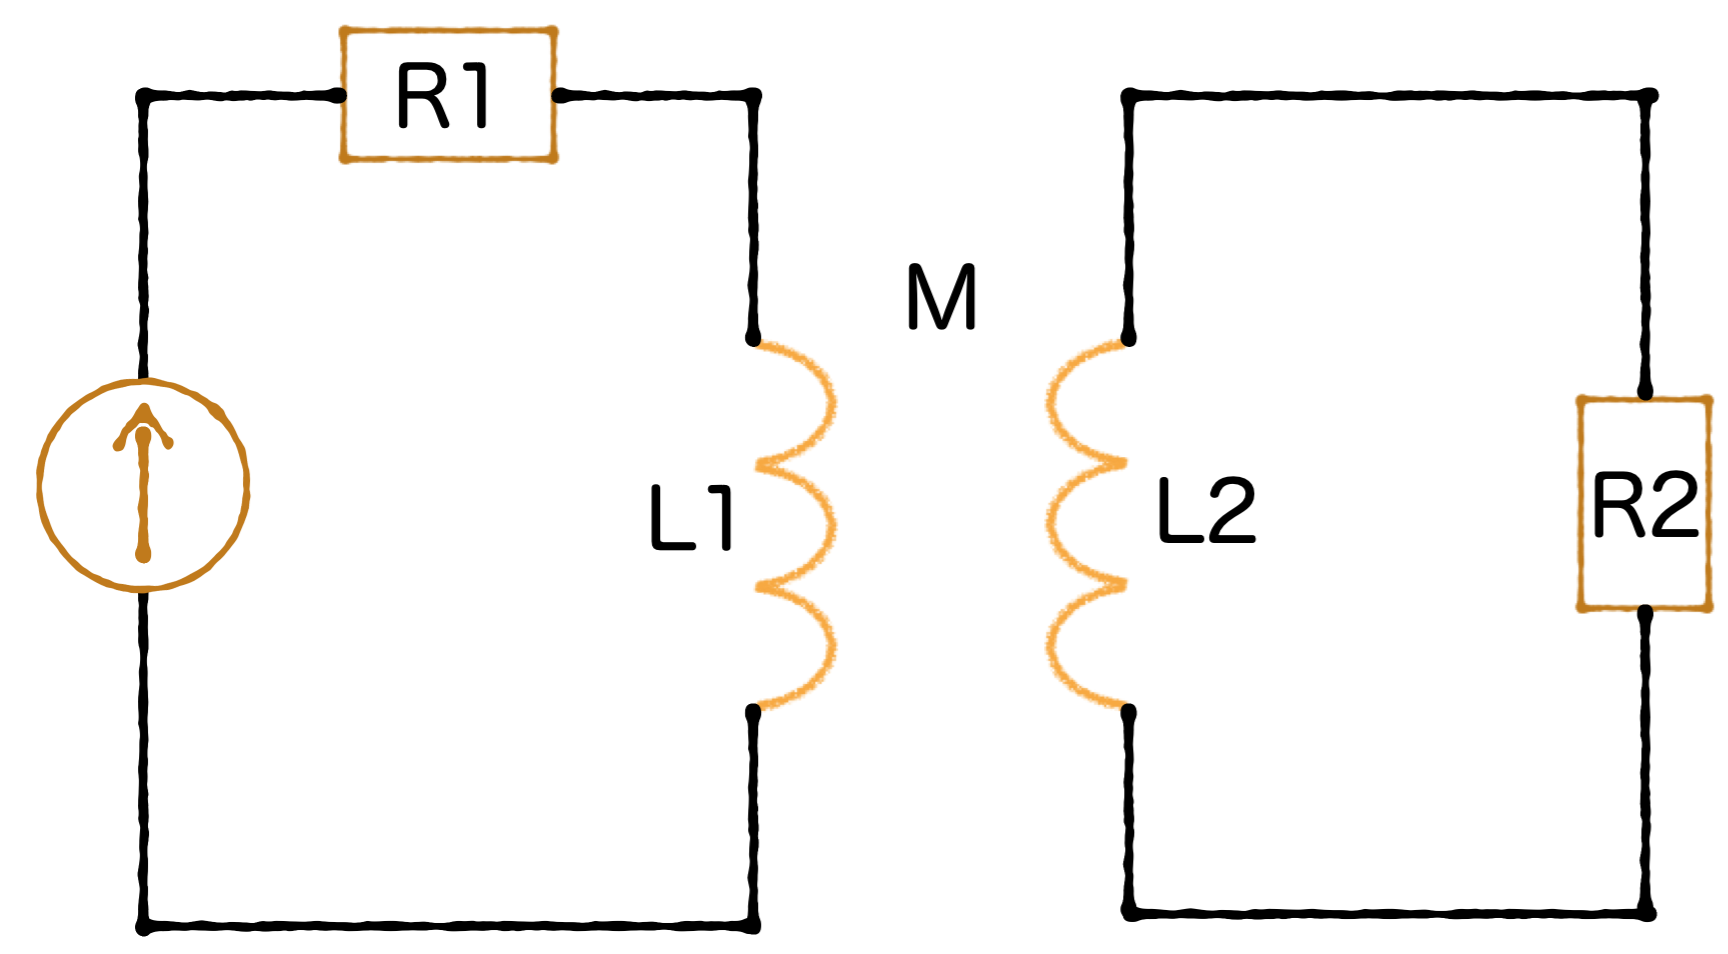
\includegraphics[width=18.5cm, bb=9 9 900 550]{./section3Effectiveness/MLGraph.png}
  \caption{The electrical circuit representing out shielding model.}
  \label{fig:circuit}
\end{figure}
In \ref{fig:circuit}, $R_1$ and $L_1$ stand for the resistance and inductance of the outer coil, and
$R_2$ and $L_2$ stand for the resistance and inductance of inner coil.
When primary current $i_1(t)$ is imposed on the outer coil,
secondary current $i_2(t)$ would be induced on the inner coil through the mutual inductance $M$ between them.
The whole differential equation can be derived as below following the Faraday's law.
\begin{equation}
  L_2\frac{di_2(t)}{dt} + R_2i_2(t) = M\frac{di_1(t)}{dt}
\end{equation}
In our experiment, due to the imposed current being trapezoid,
$M\frac{di_1(t)}{dt}$ is either $0$ or some constant.
Introducing $M\frac{di_1(t)}{dt} = v \in \mathrm{constant}$ into the above equation yields a first order inhomogeneous ordinary differential euqation.
It can be solved by conventional seperation of variables, of which the result (with the initial value considered) is shown below.
\begin{eqnarray}
  i_2(t) = (i_{2_0} &-& \frac{v_2}{R_2})\cdot \exp(-\frac{R_2}{L_2}t) + \frac{v_2}{R_2} \\
  | i_{2_0} &=& i_2(0)\nonumber
\end{eqnarray}
where $i_{2_0}$ is the initial current flowing through the inner coil.

To obtain the induced current $i_2(t)$ in every stage of the trapezoid,
we have modeled the imposed current $i_1(t)$ in all the 5 stages respectively.
The derived results are shown in the equations below.
\begin{eqnarray}
  \mathrm{region1}(t&\in&[0, t_l-\Delta t]): v_2 = 0, i_{2_0} = 0\nonumber\\
  i_2(t) &=& 0\\
  \nonumber\\
  \mathrm{region2}(t&\in&[t_l-\Delta t, t_l]): v_2 = slope_l, i_{2_0} = 0\nonumber\\
  i_2(t) &=& \frac{slope_l}{R_2}\times\left( 1 - \exp(-\frac{R_2}{L_2}(t-(t_l-\Delta t))) \right)\\
  \nonumber\\
  \mathrm{region3}(t&\in&[t_l, t_h]): v_2 = 0, i_{2_0} = i_2(t_l)\nonumber\\
  i_2(t) &=& i_2(t_l)\exp(-\frac{R_2}{L_2}(t-t_l))\\
  \nonumber\\
  \mathrm{region4}(t&\in&[t_h, t_h+\Delta t]): v_2 = slope_h, i_{2_0} = i_2(t_h)\nonumber\\
  i_2(t) &=& \left(i_2(t_h) - \frac{slope_h}{R_2}\right)\exp(-\frac{R_2}{L_2}(t-t_h)) + \frac{slope_h}{R_2}\\
  \nonumber\\
  \mathrm{region5}(t&\in&[t_h+\Delta t, \infty)): v_2 = 0, i_{2_0} = i_2(t_h+\Delta t)\nonumber\\
  i_2(t) &=& i_2(t_h+\Delta t)\exp(-\frac{R_2}{L_2}(t-(t_h+\Delta t)))
\end{eqnarray}
where $t_l$ stands for the end of the exitation, $t_h$ stands for the start of release of imposed current,
$\Delta t$ stands for the exitation time, $I_1$ stands for the peak imposed current,
and $slope_l = -slope_h = M\frac{I_1}{\Delta t}$ holds a meaning of the steepness of the exitation.

By applying Bio-Savart's law to the currents given above, we can derived the expected magnetic fields in all stages.
\begin{eqnarray}
  B(t) &=& C_1\cdot i_1(t) - C_2\cdot i_2(t)\\
  &|& C_1 = \sum_{i=1}^{N1} \frac{\mu_0r_1^2}{2\left(r_1^2 + d_i^2\right)^{\frac{3}{2}}} \in \mathrm{constant}\nonumber\\
  &|& C_2 = \sum_{i=1}^{N2} \frac{\mu_0r_2^2}{2\left(r_2^2 + d_i^2\right)^{\frac{3}{2}}} \in \mathrm{constant}\nonumber
\end{eqnarray}
The total magnetic field $B(t)$ is derived as the summation of the field produced by the inner and outer coil,
which is represented by $C_1i_1(t)$ and $C_2i_2(t)$ respectively.
The coefficients $C_1, C_2 \in \mathrm{constant}$ are parameters related to the shape of the coil,
and can be derived from Bio-Savert's law directly with simple calculation.

Substituting $i_1(t)$ and $i_2(t)$ given by equations (7)-(11) into equation (12) yields the expected field in each stage.
\begin{eqnarray}
  \mathrm{region 1}(t&\in&[0, t_l-\Delta t]):i_1(t) = 0, i_2(t) = 0\nonumber\\
  B(t) &=& 0\\
  \nonumber\\
  \mathrm{region 2}(t&\in&[t_l-\Delta t, t_l]):\nonumber\\
  &|& i_1(t) = \frac{I_1}{\Delta t}(t-t_l) + I_1\nonumber\\
  &|& i_2(t) = \frac{M}{R_2}\cdot\frac{I_1}{\Delta t}\left( 1 - \mathrm{e}^{-\frac{R_2}{L_2}(t-(t_l-\Delta t))}\right)\nonumber\\
  B(t) &=& C_1\cdot\left(\frac{I_1}{\Delta t}(t-t_l) + I_1\right) - C_2\cdot\left( \frac{M}{R_2}\frac{I_1}{\Delta t}\left( 1 - \mathrm{e}^{-\frac{R_2}{L_2}(t-(t_l-\Delta t))}\right) \right)\\
  \nonumber\\
  \mathrm{region 3}(t&\in&[t_l, t_h]):\nonumber\\
  &|& i_1(t) = I1\nonumber\\
  &|& i_2(t) = i_2(t_l)\cdot\mathrm{e}^{-\frac{R_2}{L_2}(t-t_l)}\nonumber\\
  &|& i_2(t_l) = \frac{MI_1}{R_2\Delta t}\left( 1-\mathrm{e}^{-\frac{R_2}{L_2}\Delta t} \right)\in \mathrm{constant}\nonumber\\
  B(t) &=& C_1\cdot I_1 - C_2\cdot\frac{MI_1}{R_2\Delta t}\left( 1-\mathrm{e}^{-\frac{R_2}{L_2}\Delta t} \right)\mathrm{e}^{-\frac{R_2}{L_2}(t-t_l)}
\end{eqnarray}
\begin{eqnarray}
  \mathrm{region 4}(t&\in&[t_h, t_h+\Delta t]):\nonumber\\
  &|& i_1(t) = I_1\left( 1-\frac{t-t_h}{\Delta t} \right)\nonumber\\
  &|& i_2(t) = \left( i_2(t_h)+\frac{MI_1}{R_2\Delta t}\right)\mathrm{e}^{-\frac{R_2}{L_2}(t-t_h)} - \frac{MI_1}{R_2\Delta t} \nonumber\\
  &|& i_2(t_h) = \frac{MI_1}{R_2\Delta t}\left( 1-\mathrm{e}^{-\frac{R_2}{L_2}\Delta t} \right)\mathrm{e}^{-\frac{R_2}{L_2}(t_h-t_l)}\in\mathrm{constant}\nonumber\\
  B(t) &=& C_1\cdot I_1\left( 1-\frac{t-t_h}{\Delta t} \right) - C_2\cdot\left( \left(i_2(t_h)+\frac{MI_1}{R_2\Delta t}\right)\mathrm{e}^{-\frac{R_2}{L_2}(t-t_h)} - \frac{MI_1}{R_2\Delta t} \right)\\
  \nonumber\\
  \mathrm{region 5}(t&\in&[t_h+\Delta t, \infty)):\nonumber\\
  &|& i_1(t) = 0\nonumber\\
  &|& i_2(t) = i_2(t_h+\Delta t)\mathrm{e}^{-\frac{R_2}{L_2}(t-(t_h+\Delta t))}\nonumber\\
  &|& i_2(t_h+\Delta t) = \frac{MI_1}{R\Delta t}\nonumber\\
  &\cdot&\left(\left( 1 -\mathrm{e}^{-\frac{R_2}{L_2}\Delta t} \right)\mathrm{e}^{-\frac{R_2}{L_2}(t_h-t_l)} + \mathrm{e}^{-\frac{R_2}{L_2}\Delta t} - 1 \right)\nonumber\\
  B(t) &=& -C_2\cdot i_2(t_h+\Delta t)\mathrm{e}^{-\frac{R_2}{L_2}(t-(t_h+\Delta t))}
\end{eqnarray}
To make theese equations clear, we have introduced three parameters with physical meaning.
\begin{eqnarray}
  \tau &=& \frac{L_2}{R_2} \mathrm{(time constant)}\\
  \alpha &=& C1\cdot I1 \mathrm{(field produced by the outer coil)}\\
  \beta &=& C2\cdot\frac{MI_1}{R_2\Delta t} \mathrm{(field produced by the inner coil)}
\end{eqnarray}
Introducing theese parameters into equation (13)-(17) yields
\begin{eqnarray}
  \mathrm{region1}(t&\in&[0, t_l-\Delta t]):\nonumber\\
  B(t) &=& 0\\
  \nonumber\\
  \mathrm{region2}(t&\in&[t_l-\Delta t, t_l]):\nonumber\\
  B(t) &=& \alpha\left(\frac{t-t_l}{\Delta t} + 1\right) - \beta\left( 1 - \mathrm{e}^{-\frac{R_2}{L_2}(t-(t_l-\Delta t))}\right)\\
  \nonumber\\
  \mathrm{region3}(t&\in&[t_l, t_h]):\nonumber\\
  B(t) &=& \alpha - \beta\left( 1-\mathrm{e}^{-\frac{\Delta t}{\tau}} \right)\mathrm{e}^{-\frac{t-t_l}{\tau}}\\
  \nonumber\\
  \mathrm{region4}(t&\in&[t_h, t_h+\Delta t]):\nonumber\\
  B(t) &=& \alpha\left( 1-\frac{t-t_h}{\Delta t} \right) - \left( \beta\left(1-\mathrm{e}^{-\frac{\Delta t}{\tau}}\right)\mathrm{e}^{-\frac{t_h-t_l}{\tau}} + \beta \right)\mathrm{e}^{-\frac{t-t_h}{\tau}} + \beta\\
  \nonumber\\
  \mathrm{region5}(t&\in&[t_h+\Delta t, \infty)):\nonumber\\
  B(t) &=& -\beta\left( \left(1-\mathrm{e}^{-\frac{\Delta t}{\tau}}\right)\mathrm{e}^{-\frac{t_h-t_l}{\tau}} + \mathrm{e}^{-\frac{\Delta t}{\tau}} -1 \right) \times\mathrm{e}^{-\frac{t-(t_h+\Delta t)}{\tau}}
\end{eqnarray}
Theese equations (21)-(25) describes the expected magnetic field at the central point if imposed by trapezoid current on the outer coil.


\subsubsection{Method}
A series of experiments have been conducted to measured the time constant.
The experimental equipments are shown in Fig. \ref{fig:experimentalEquipments}.
\begin{figure}[H]
  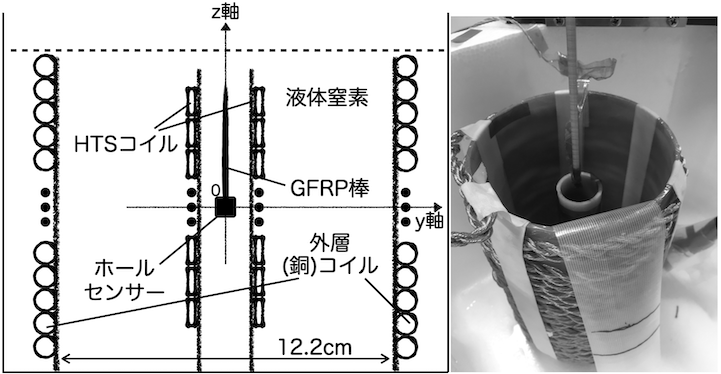
\includegraphics[width=18.5cm, bb=9 9 900 550]{./section3Effectiveness/experimentalEquipments.png}
  \caption{The experimental equipments. (left) The schematic drawing; (right) The photo of which.}
  \label{fig:experimentalEquipments}
\end{figure}
The experiment is conducted in the following procedure on two coils,
one having a small radius and long length, the other owning the opposite.
The specification of the coils is shown in Tab. \ref{tab:expSpecification}.
\begin{enumerate}
  \item Imposed trapezoid current on the outer coil.
  \item Measured the time variation of the central magnetic field.
  \item Fit the measured curve by equation (21)-(25) to find the three paraeters $\tau, \alpha, \beta$.
  \item Repeat on different imposed current.
\end{enumerate}
\begin{table}[H]
  \centering
  \caption{Specification of the experiment.}
  \label{tab:expSpecification}
  \begin{tabular}{cccc}\hline\hline
    Parameter & Inner Coil1 & Inner Coil2 & Outer Coil \\\hline
    Diameter [cm] & 8.8 & 3.0 & 12.2\\\hline
    Length [cm] & 1.2 & 10 & 17.8 \\\hline
    Turns & 2 & 50 & 27 \\\hline
    Critical Current $I_C$ [A] & 500 & 30 & Copper \\\hline
    Width of Superconductor Tape & 12 & 4 & -
  \end{tabular}
\end{table}

\subsubsection{Result and Discussion}
Results of measuring time constants of Coil1 and Coil2 are shown in Fig. \ref{fig:Coil1TimeConstant} and Fig. \ref{fig:Coil2TimeConstant}.
\begin{figure}[H]
  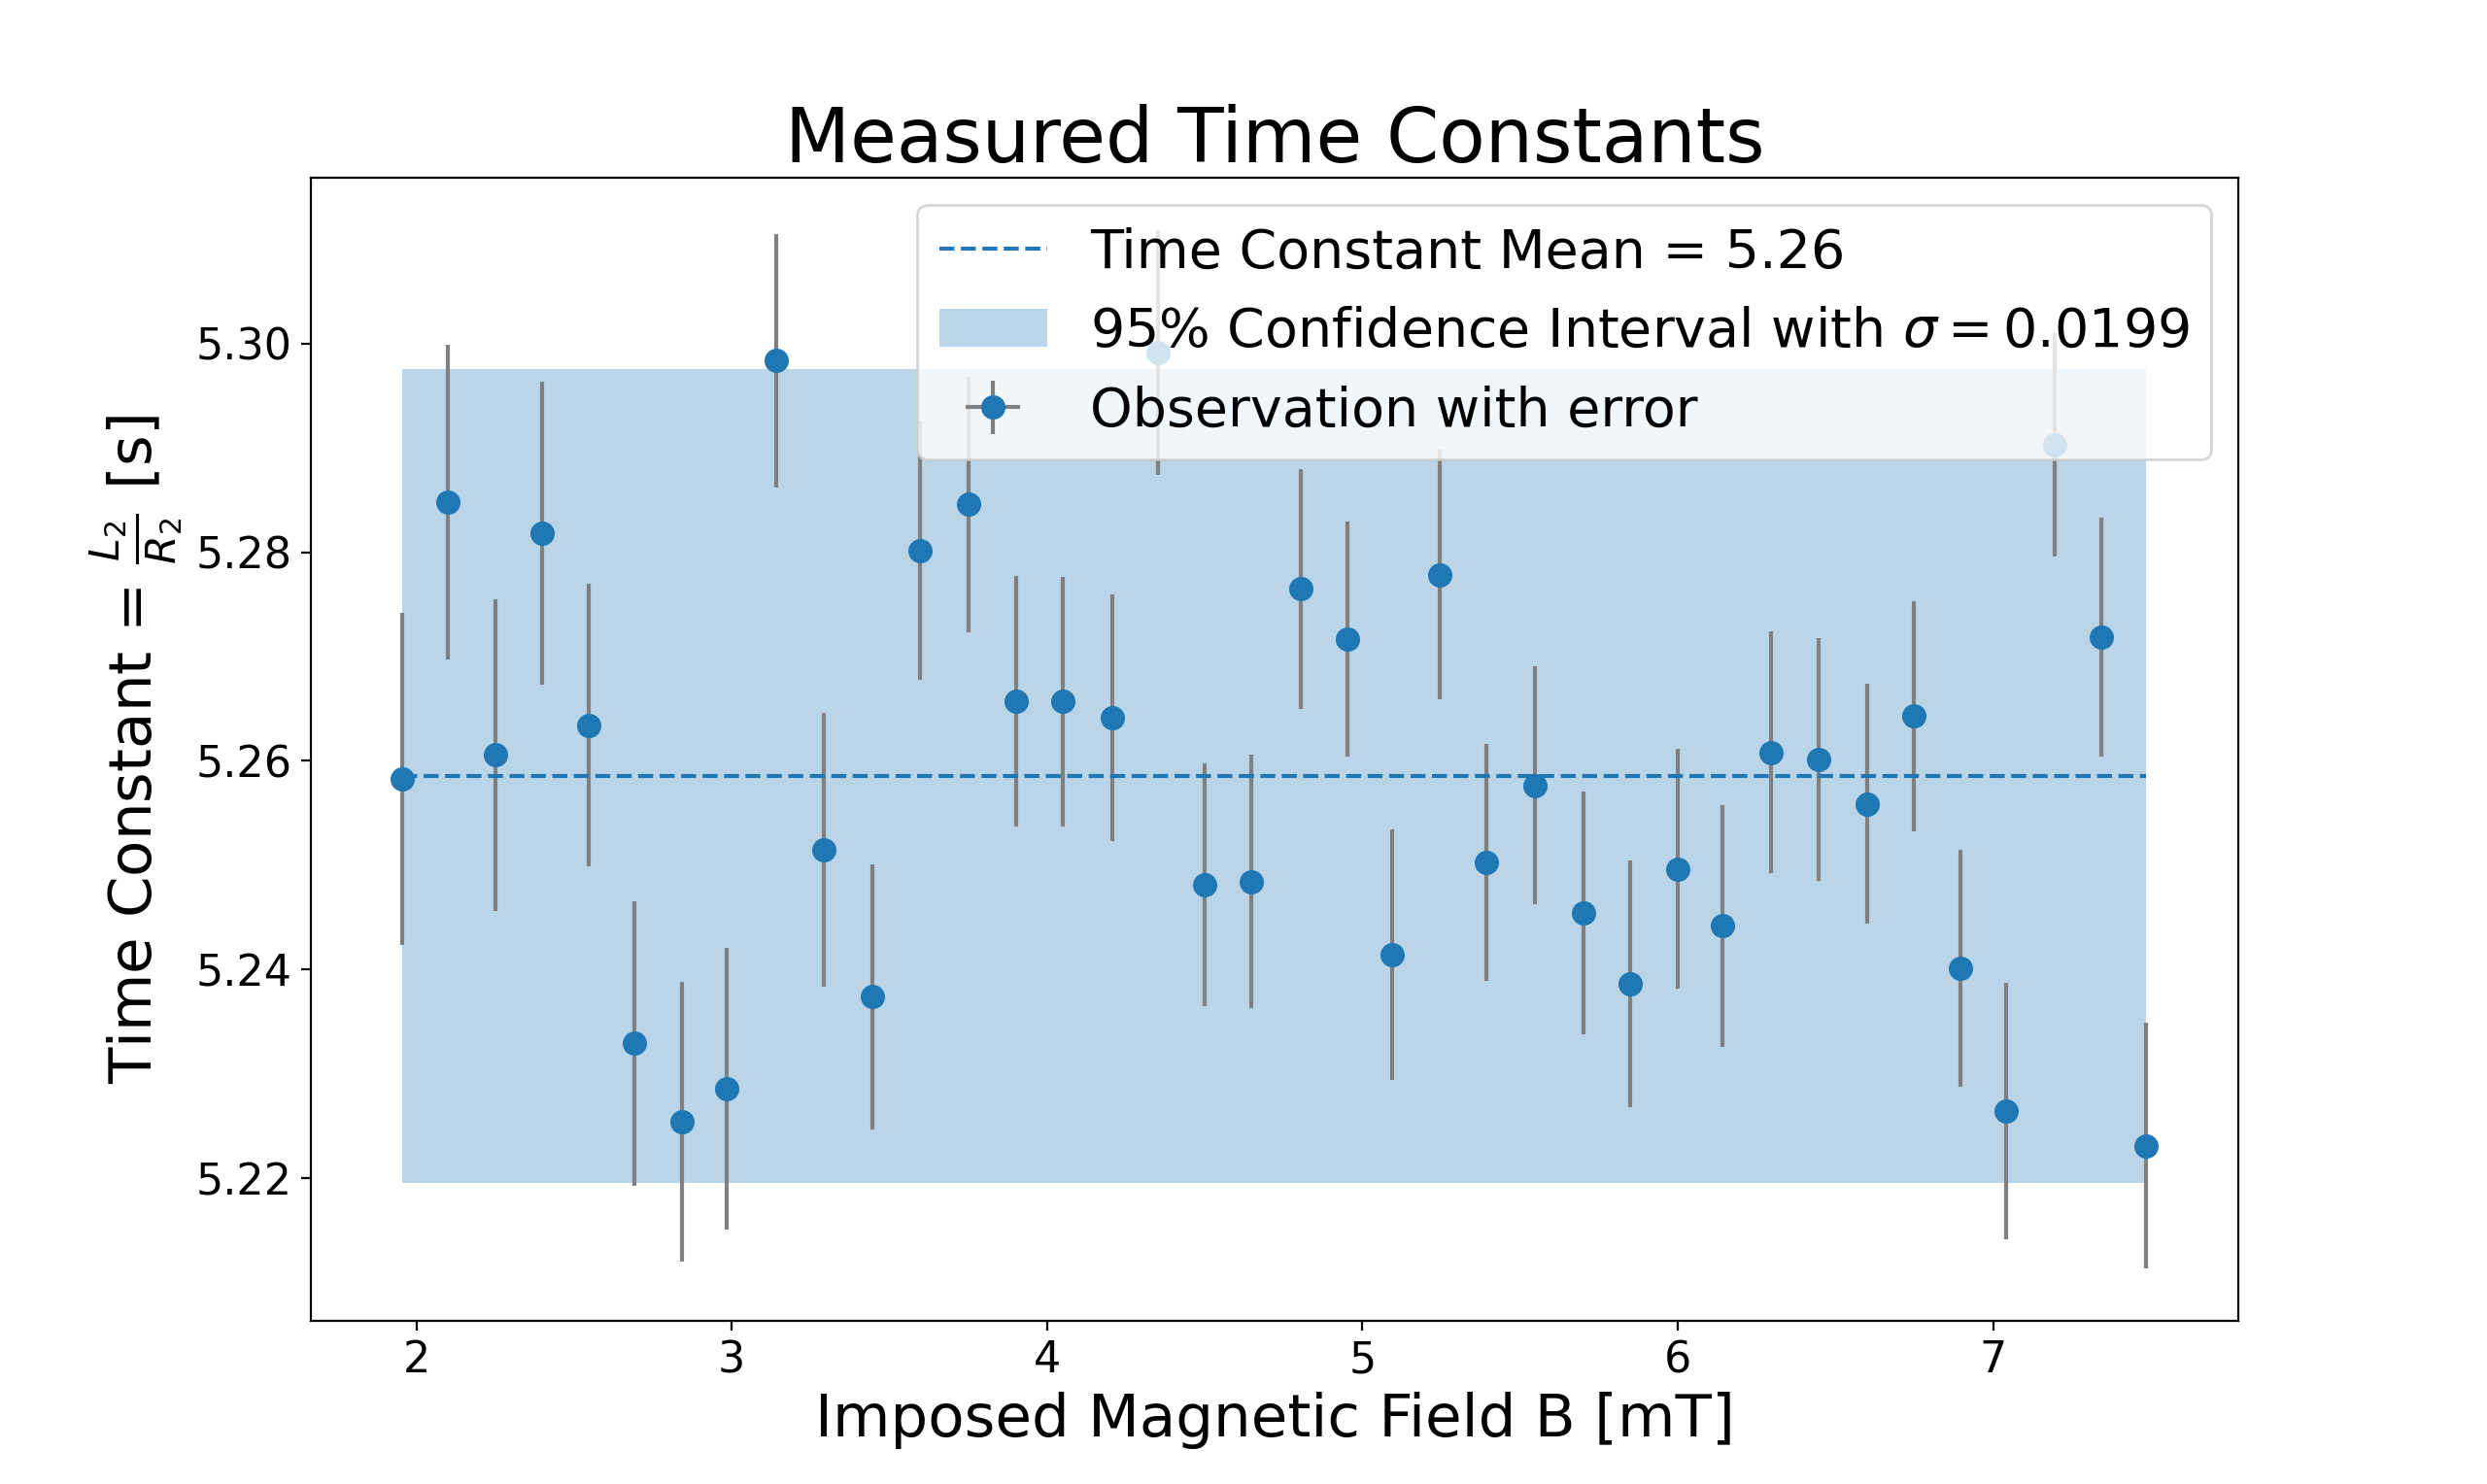
\includegraphics[width=17cm, bb=9 9 900 520]{./section3Effectiveness/Coil1TimeConstant.png}
  \caption{The measured time constant of coil1.}
  \label{fig:Coil1TimeConstant}
\end{figure}
\begin{figure}[H]
  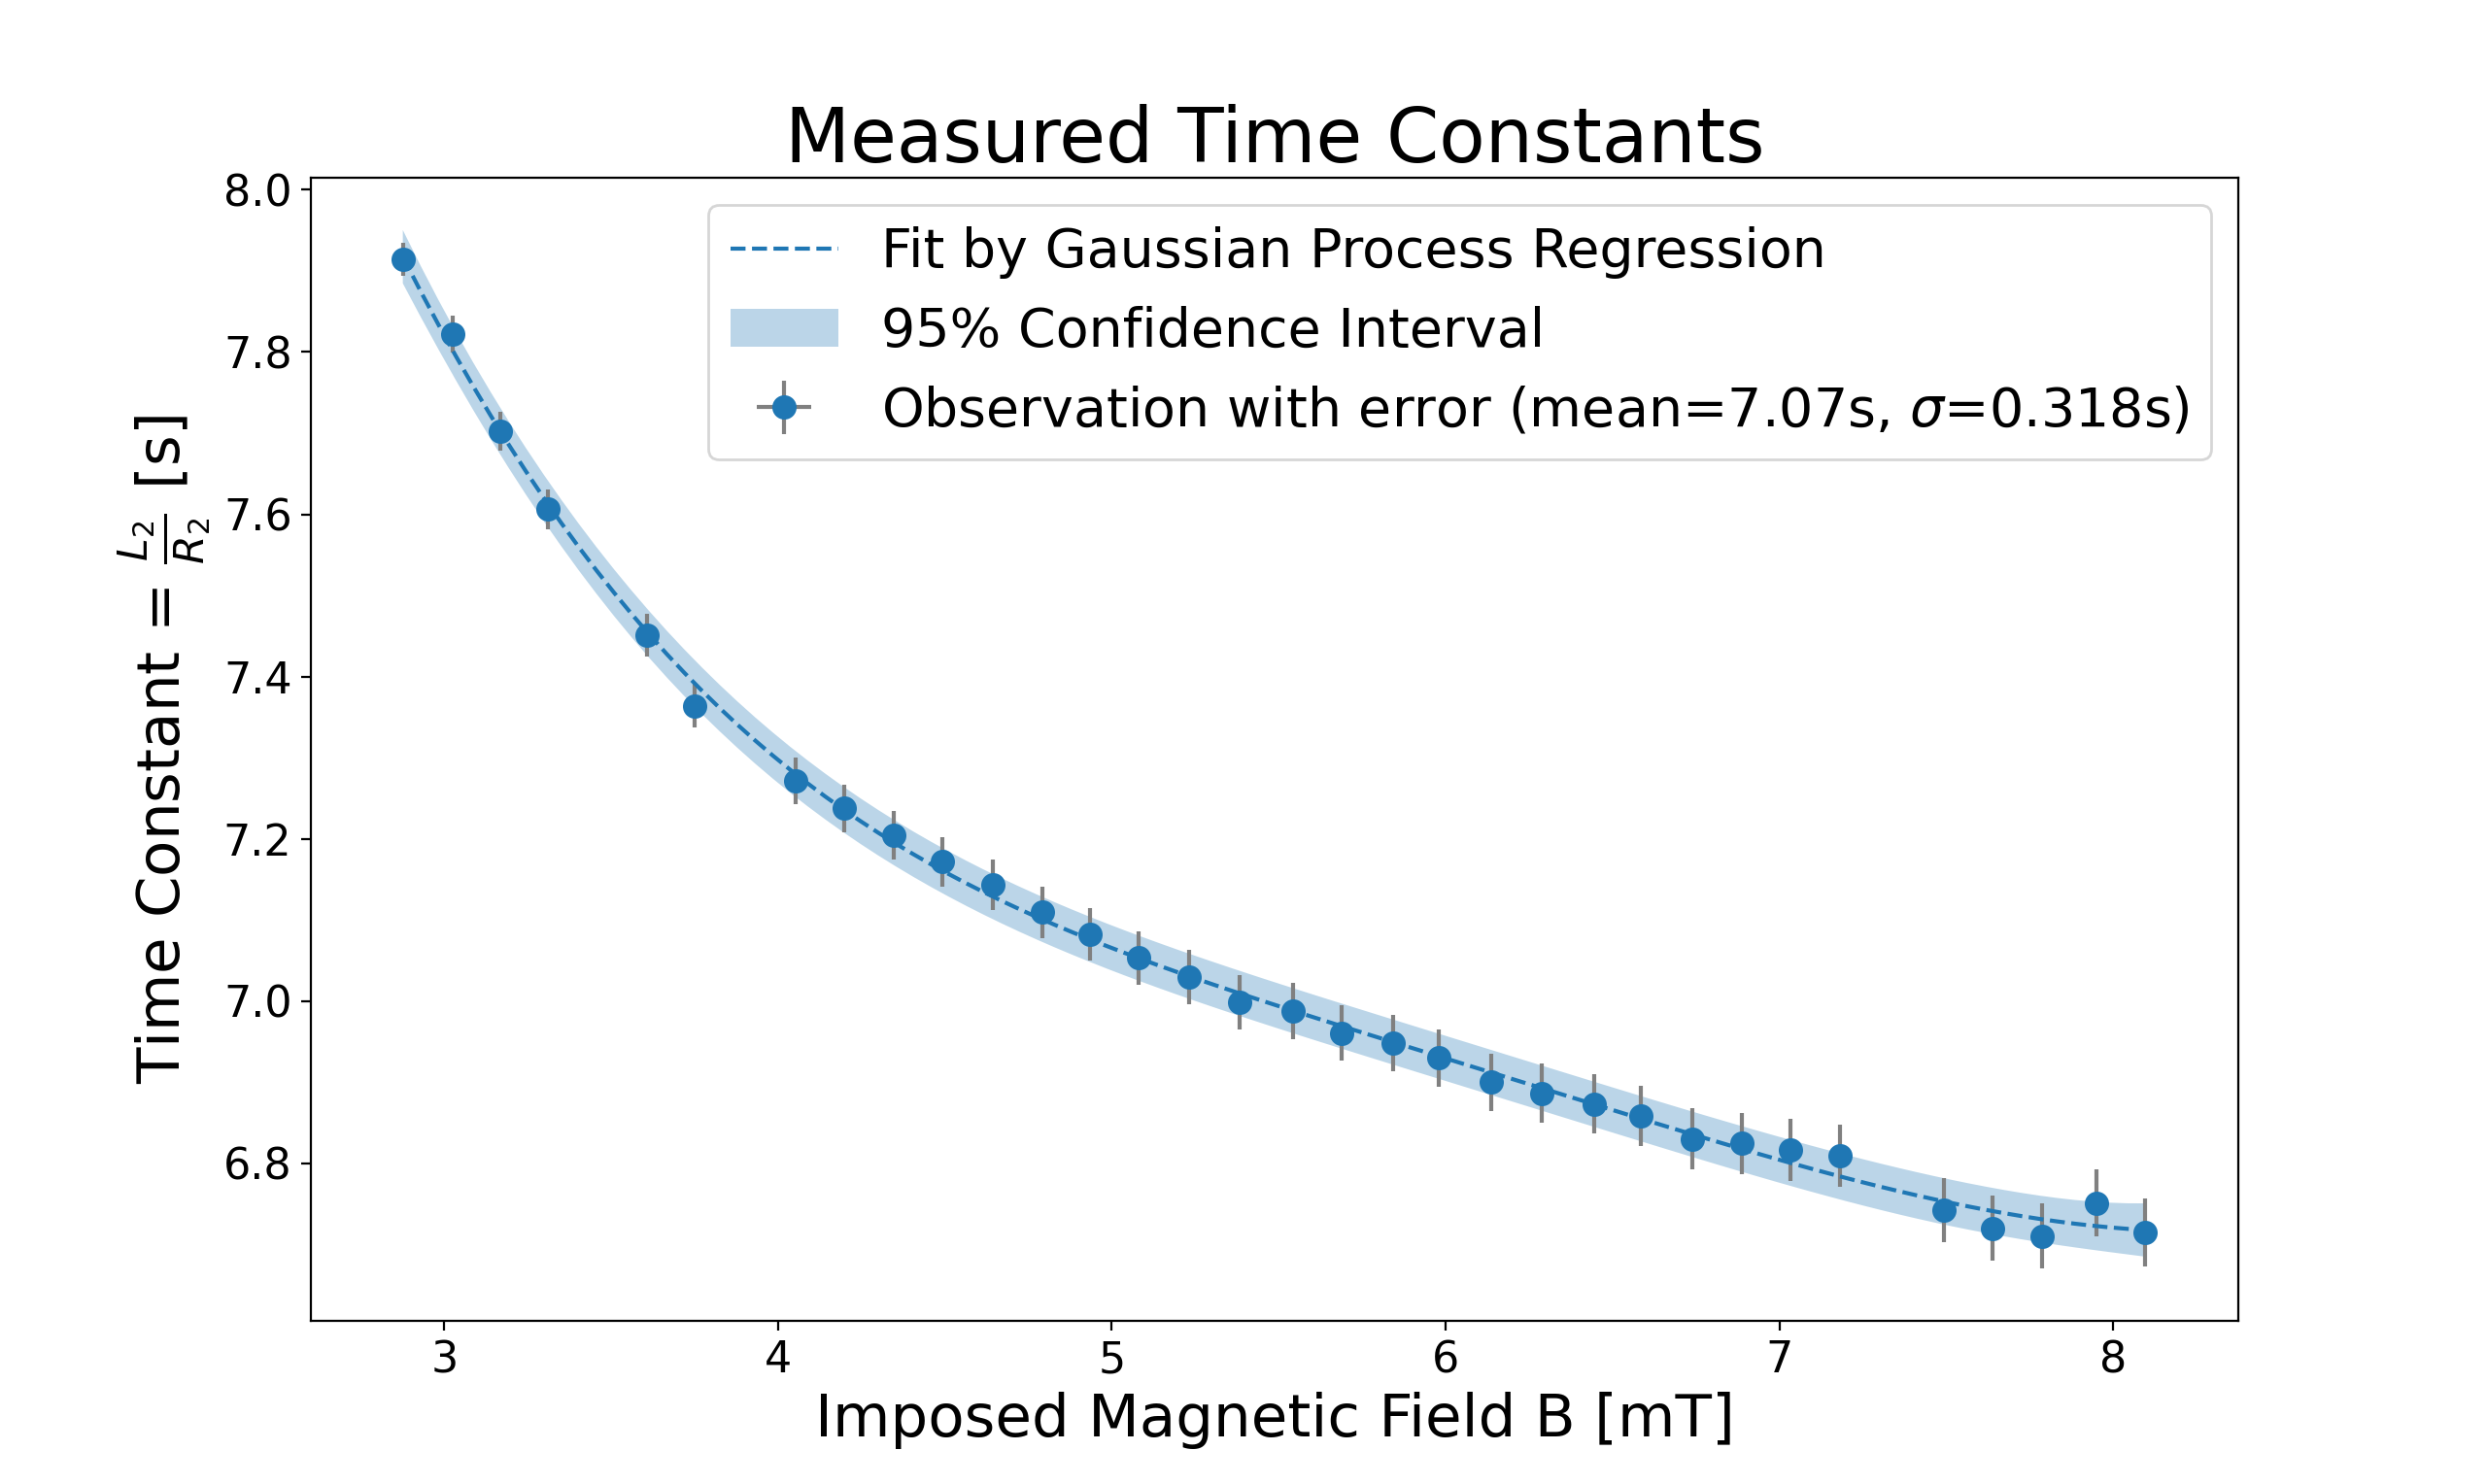
\includegraphics[width=17cm, bb=9 9 900 480]{./section3Effectiveness/Coil2TimeConstant.png}
  \caption{The measured time constant of coil2.}
  \label{fig:Coil2TimeConstant}
\end{figure}
The measured time constant of Coil1 is about $5$ seconds, while that of Coil2 is about $7$ seconds.
In electrical circuits consist of inductance and resistance, the time constant can be written as $\tau = \frac{L}{R}$
Obviously, the difference between them result from the different inductance and resistance of them.
Coil2 has more turns than Coil1, which increases the time constant, but is slightly canceled out by its thinner contact area,
which reduces its time constant.
Besides, the measurement conducted on Coil1 seems to be more stable along different imposed fields,
which in turn gives a more accurate result.
The reason why the time constant of Coil2 shows a magnetic field related property,
which shouldn't happend since both the inductance and the resistance relate only to the shape of coil not the current or any field,
is worth discussed.
One possible hypothesis is due to the non-linearity resistance observed widely on high temperature superconductors.
If we plotted the V-I diagram on superconductor, we would obtain a curve not a straight line,
which indicates the resistance $R = V/I$ is not linear.
Also, When current flow through a superconductor tape increases,
it tends to gather around the surface, which may cause a current related change on inductance.
Either change on the inductance or the resistance will alter the time constant,
this may considered a propper theory.

Besides, another possible reason which rises from the fitting algorithm can be considered.
Since we fit the three parameters from the data simultaneously,
an equaled amount of information on each parameter should be provided properly.
For instance, if a model aimed to recognize either a picture is showing a dog or a cat is trained by 90 dog pictures and 10 cat pictures,
the model tends to give a 90$\%$ guess on dog given any picture,
which is extremely inaccurate.
This is known as the "overfitting" on machine learning field.
In our experiment, we have used the imposed current - measured magnetic field data to find the three parameters,
an equaled amount of information given on them should be guaranteed.

Before we closed this section, the obtained result would be compared with the full scale model to answer the key question:
Is the time constant large enough?
In Fig. \ref{fig:Coil1TimeConstant} and Fig. \ref{fig:Coil1TimeConstant}, we have measured a time constant of a few seconds in both coils.
In our scaled down coils, due to the small inductance and the relatively large electrical resistance,
small time constants of a few seconds are measured.
In a full scale model, for instance a spaceshuttle, the coil becomes enormous and thus owns large inductance and low relatively resistance.
Here we conduct a simple calculation using the specification of the spaceshuttle Columbia,
of which the length is $37.24$ m, the radius is $17.86$ m.
From a conservative perspective, we gave it an 80\% discount.
Using the measured inductance and resistance in the scaled down model,
we are able to derive the full scale time constant as shown below.
\begin{eqnarray}
  \Phi &=& 17.86[\mathrm{m}] \times 80\% = 14.29[\mathrm{m}] \\\nonumber
  \mathrm{length} &=& 37.24[\mathrm{m}] \times 80\% = 29.79[\mathrm{m}] \\\nonumber
  L_{\mathrm{fullScale}} &=& k_N\cdot\frac{\mu N^2\pi r^2}{\mathrm{length}}\cong21.8 [\mathrm{H}] \\\nonumber
  \tau_{\mathrm{real}} &=& \tau_{\mathrm{scaledDown}}\cdot\frac{L_{\mathrm{real}}}{L_\mathrm{scaledDown}} = 5.26[\mathrm{sec}]\cdot\frac{21.8[\mathrm{H}]}{0.4[\mathrm{\mu H}]}\cong 8.7[\mathrm{year}]
\end{eqnarray}
From equation (), a time constant of a few years in a full scale model can be derived,
which indicates that the induced current should retain for a few years making the shielding system feasible.

\subsubsection{Conclusion}
In this section, to give an approximation on the time constant of a full scale model used in space crafts,
we have conducted experiments on 2 scaled down model coil and measured their time constants.
According to the results shown in Fig. \ref{fig:Coil1TimeConstant} and Fig. \ref{fig:Coil1TimeConstant},
the time constants are a few seconds in the scaled down models,
and are calculated to be a few years in a full scale model.
The result infers that the induced current should maintain strengthful for a few years,
showing that the shielding system is capable of working for long enough on every exitation.


\newpage
\subsection{Shielding Ability}
Besides having a large time constant,
performing enough shielding ability is also a critical factor when working as a shielding system.
To testify this property,  a series of experiments have been conducted on mutiple coils.
In this section, we would denote the theory and methods of our experiments as well as the obtain results and the comparison to the full scale model.

\subsubsection{Purpose}
The purpose of this exam is to testify whether the proposed Electromagnetic Induction Type Magnetic Cloak has enough shielding ability.
In theory, shielding rates could reach as high as 99\%, which means shielding 1 T external field to 10 mT is possible.
For convenience, we only take the axis shielding rate into evaluation,
since the measured field in the entire internal space would be no difference beyond 10\%.

\subsubsection{Theory}
The entire circuit is the same as Fig. \ref{fig:experiment} in section 3.1 except for the imposed current being AC instead of DC.
If AC current $i_1(t) = I_1\sin(\omega t)$ is imposed, equation (5) becomes a classic Bernoulli equation,
which can be solved by introducing propper intergrating factor.
The general solution with initial value involved is shown below.
\begin{eqnarray}
  i_2(t) &=& \mathrm{e}^{-h(t)}\left( \int \mathrm{e}^{h(t)}\cdot r(t)dt + C_0 \right)\nonumber\\
  &|& h(t) = \frac{R_2}{L_2}t, r(t) = \frac{M}{L_2}\cdot I_1\omega\cos(\omega t) \nonumber\\
  &=& \frac{\frac{M}{L_2}\omega I_1}{(\frac{R_2}{L_2})^2+\omega^2}\left(\frac{R_2}{L_2}\right)\mathrm{e}^{-\frac{R_2}{L_2}t} \nonumber\\
  &+& \frac{\frac{M}{L_2}\omega I_1}{(\frac{R_2}{L_2})^2+\omega^2}\left(\frac{R_2}{L_2}\cos(\omega t) + \omega\sin(\omega t)\right)
\end{eqnarray}
This equation describes the induced current $i_2(t)$ when imposed by sin wave.
In equation (27), the first term refers to the transient phenomena with time constant $\tau$,
while the second term represents the steady state.
If the frequency is relatively large $\omega \gg \frac{R_2}{L_2}$,
$i_2(t)$ becomes strictly sin wave shown below,
which agrees with the solution from phasor calculation.
\begin{equation}
  i_2(t) = \frac{MI_1}{L_2}\cdot\sin(\omega t) |\omega \gg \frac{R_2}{L_2}
\end{equation}
By equation (28), we are able to derive the central magnetic field $B(t)$ as below.
\begin{eqnarray}
  B(t) &=& C_1\cdot i_1(t) - C_2\cdot i_2(t)\nonumber\\
  &|& C_1 = \sum_{i=1}^{N1} \frac{\mu_0r_1^2}{2\left(r_1^2 + d_i^2\right)^{\frac{3}{2}}} \in \mathrm{constant}\nonumber\\
  &|& C_2 = \sum_{i=1}^{N2} \frac{\mu_0r_2^2}{2\left(r_2^2 + d_i^2\right)^{\frac{3}{2}}} \in \mathrm{constant}\nonumber\\
  &|& i_1(t) = I_1\sin(\omega t)\nonumber\\
  &|& i_2(t) = \frac{MI_1}{L_2}\cdot\sin(\omega t)\nonumber\\
  &=& C_1\cdot I_1\sin(\omega t) - C_2\cdot\frac{MI_1}{L_2}\sin(\omega t)|\omega \gg \frac{R_2}{L_2}
\end{eqnarray}
where the first term represents the field generated by the external coil,
and the second term represents the field generated by the internal coil.
We can further derive the centeral shielding rate to be
\begin{equation}
  \mathrm{Shielding Rate} = \frac{C_2\cdot i_2(t)}{C1\cdot i_1(t)} = \frac{C_2}{C_1}\cdot\frac{M}{L_2}
\end{equation}
Surprisingly, according to equation (30),
the shielding rate only depends on the shape of the external coil ($C_1$),
the shape of the internal coil ($C_2$),
the mutual inductance between them ($M$),
and the inductance of the internal coil ($L_2$).
Note that given a fix shape external coil,
the shielding rate would be defined by $\frac{C_2M}{L_2}$,
and thus we can't tell anything about how the shielding rate would change when the size of internal coil decreases.
It needs to be calculated case by case, which may become annoying on the system desing.
The detail of coefficients $C_1$ and $C_2$ have already been shown in equation (12).
The derivation of $M$ and $L$ would be shown in the following paragraph.


\begin{figure}[H]
  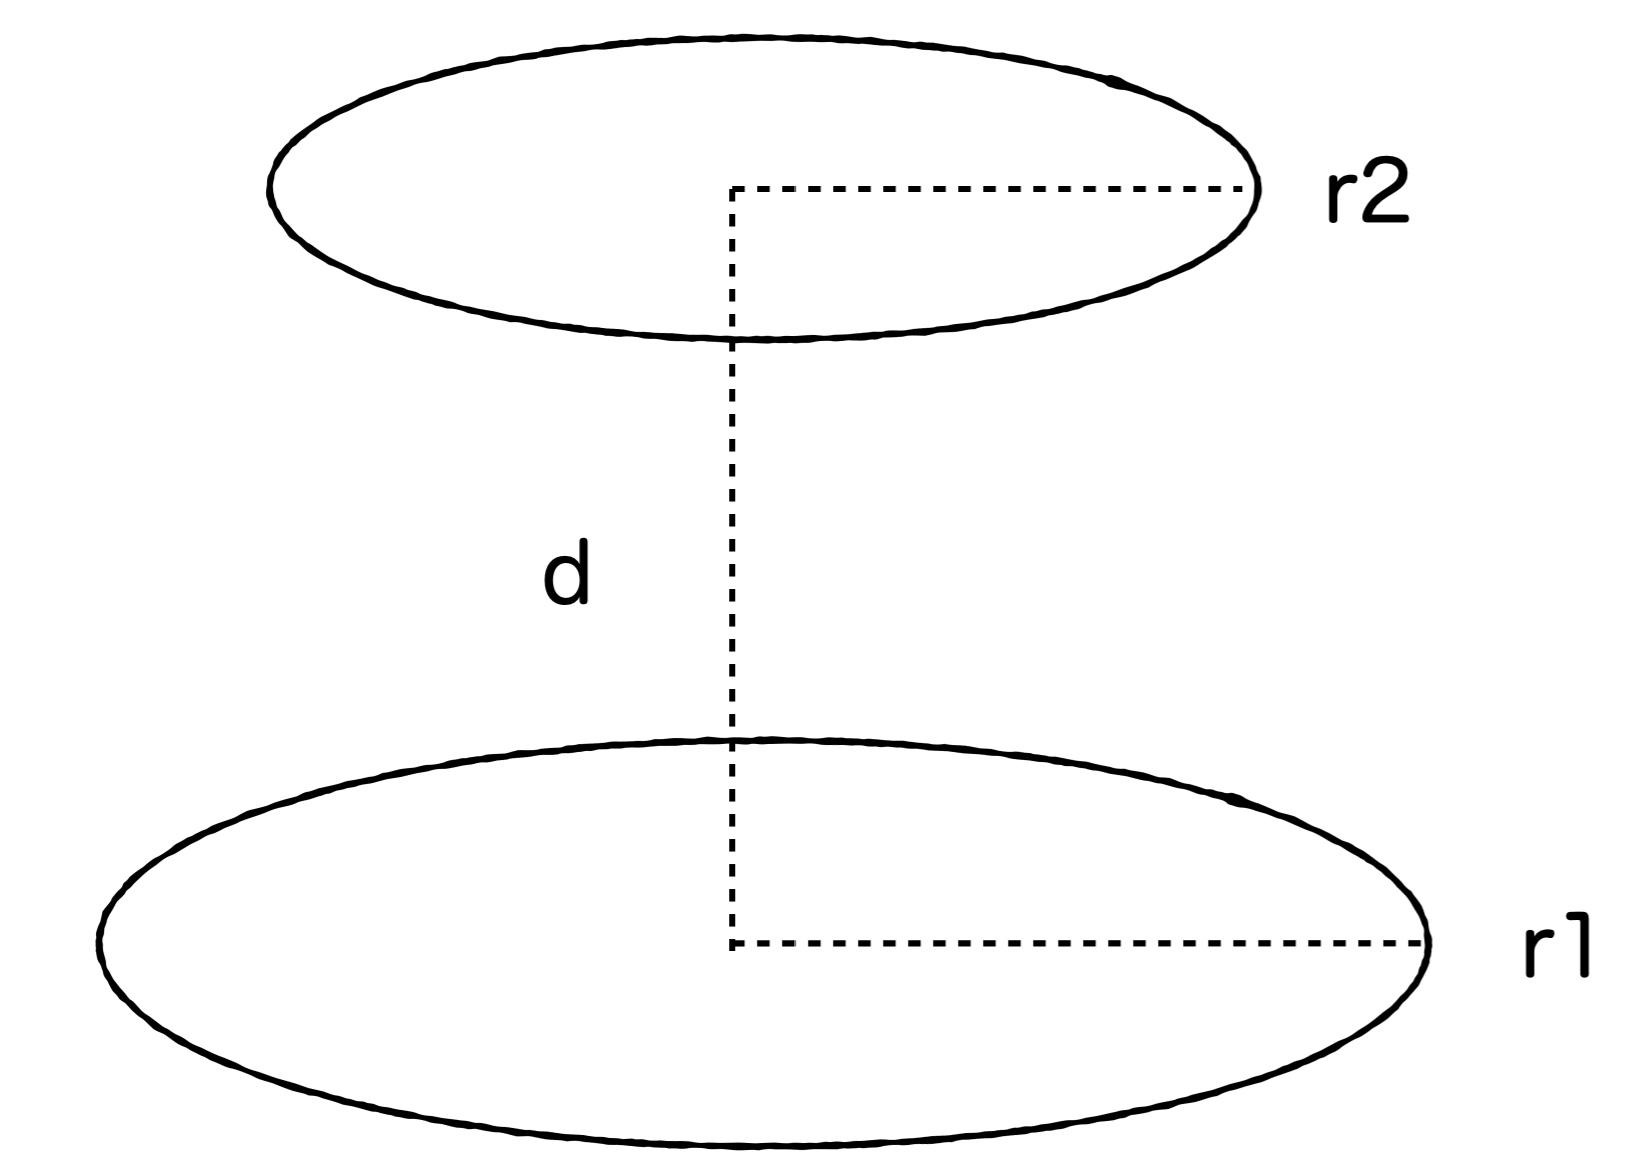
\includegraphics[width=17cm, bb=9 9 900 550]{./section3Effectiveness/2CoilsExample.png}
  \caption{A schematic diagram of mutal inductance derived from 2 loops.}
  \label{fig:M}
\end{figure}
Imagine two conductive loops with radius $r_1$ and $r_2$ respectively, placed parallelly by distance $d$ like Fig. \ref{fig:M}.
The mutual inductance between them could be derived from Neumann's formula.
\begin{eqnarray}
  M(r_1, r_2, d) &=& \frac{\mu_0}{4\pi}\int_0^{2\pi}\int_0^{2\pi} \frac{r_1r_2\cos(\theta-\theta')d\theta d\theta'}{\sqrt{r_1^2 + r_2^2 + d^2 - 2r_1r_2\cos(\theta-\theta')}} \nonumber\\
  &=& \frac{\mu_0}{2}\int_0^{2\pi} \frac{r_1r_2\cos(\phi) d\phi}{\sqrt{r_1^2 + r_2^2 + d^2 - 2r_1r_2\cos(\phi)}}
\end{eqnarray}
This integral couldn't be solved with only elementary functions,
but by introducing elliptic integral it can be rewritten into closed form,
as shown in equation (32).
\begin{eqnarray}
  M(r_1, r_2, d) &=& \mu_0\sqrt{r_1r_2}\left( (\frac{2}{k}-k)K(k) - \frac{2}{k}E(k) \right)\\
  &|& k = \sqrt{\frac{4r_1r_2}{(r_1+r_2)^2 + d^2}}\nonumber\\
  &|& K(k) = \mathrm{The first kind complete elliptic integral with modulus} k\nonumber\\
  &|& E(k) = \mathrm{The second kind complete elliptic integral with modulus} k\nonumber
\end{eqnarray}
Equation (32) denotes the mutual inductance between two loops from the first principles.
For the mutual inductance between two multi-turn coils,
applying equation (32) to all their turn would raise the total mutual inductance.
\begin{eqnarray}
  \sum M &=& \sum_{i=1}^{N_1\cdot N_2}\mu_0\sqrt{r_1r_2}\left( (\frac{2}{k_i}-k_i)K(k_i) - \frac{2}{k_i}E(k_i) \right)\nonumber\\
  &|& k = \sqrt{\frac{4r_1r_2}{(r_1+r_2)^2 + d_i^2}}
\end{eqnarray}
where $d_i$ refers to the central distance betwenn the specific turns,
$N_1$ and $N_2$ refer to the turns of the each coil.
Equation (33) represents the mutual inductance $M$ between $N_1$ turns external coil and $N_2$ turns internal coil.


Next, we derive the inductance $L$ of a finite length $l$ solenoid coil with radius $r$, $N$ turns.
First, the inductance of an infinite solenoid coil $l \to \infty$ is well known as $L = \frac{\mu N^2\pi r^2}{l}$.
When the length is finite, a coefficient $K_N$ ranging from $0\sim1$, named after Nagaoka Hanntaro, should be multiplied.
\begin{eqnarray}
  L&(&r, l) = K_N\cdot\frac{\mu N^2\pi r^2}{l}\\
  &|& K_N = \frac{4}{3\pi\sqrt{1-n^2}}\left( \frac{1-n^2}{n^2}K(n) - \frac{1-2n^2}{n^2}E(n) - n \right)\nonumber\\
  &|& n(r, l) = \frac{1}{\sqrt{(\frac{l}{2r})^2 + 1}}\nonumber\\
  &|& K(n) = \mathrm{TheFirstKindCompleteEllipticIntegralWithModulus} k\nonumber\\
  &|& E(n) = \mathrm{TheSecondKindCompleteEllipticIntegralWithModulus} k\nonumber
\end{eqnarray}
Equation (34) represents the inductance of a $N$ turns, radius $r$, and relatively short length solenoid coil.


Using the equations described in section 3.2.1-3.2.2,
we are able to write the shielding rate from foundamental coil parameters.
\begin{eqnarray}
  \mathrm{Shielding Rate}&(&r_1, l_1, N_1, r_2, l_2, N_2) = \frac{C_2}{C_1}\times\frac{M}{L_2}\\
  &=& \frac{\sum_{i=1}^{N1} \frac{\mu_0r_1^2}{2\left(r_1^2 + d_i^2\right)^{\frac{3}{2}}}}{\sum_{i=1}^{N2} \frac{\mu_0r_2^2}{2\left(r_2^2 + d_i^2\right)^{\frac{3}{2}}}}\nonumber\\
  &\times& \frac{\sum_{i=1}^{N_1\cdot N_2}\mu_0\sqrt{r_1r_2}\left( (\frac{2}{k_i}-k_i)K(k_i) - \frac{2}{k_i}E(k_i) \right)}{K_N\cdot\frac{\mu N^2\pi r^2}{l}}\nonumber
\end{eqnarray}
Given an external coil (radius $r_1$, turns $N_1$, length $l_1$),
and an internal coil (radius $r_2$, turns $N_2$, length $l_2$),
equation (35) explains the central shielding rate when external coil is imposed by $i_1(t) = I_1\sin(\omega t)$.
The shielding rate here is defined as, the field generated by internal coil devided by the field generated by external coil.
As well, equation (35) holds when the frequency $\omega$ is extremely larger than $\tau=\frac{R_2}{L_2}$ is satisfied.

Just as described in 3.2.1, the shielding rate depends on the shapes of both coils and grows nonlinearly,
which is hard to imagine.
To give a schematic picture of it, we have calculated some shielding rates under various internal coils and a fix external coil,
using equation ().
Fig. \ref{fig:simulatedShieldingRates3D1} and \ref{fig:simulatedShieldingRates3D2} shows the same simulated result,
from different angle.
Fig. \ref{fig:overshielding}
\begin{figure}[H]
  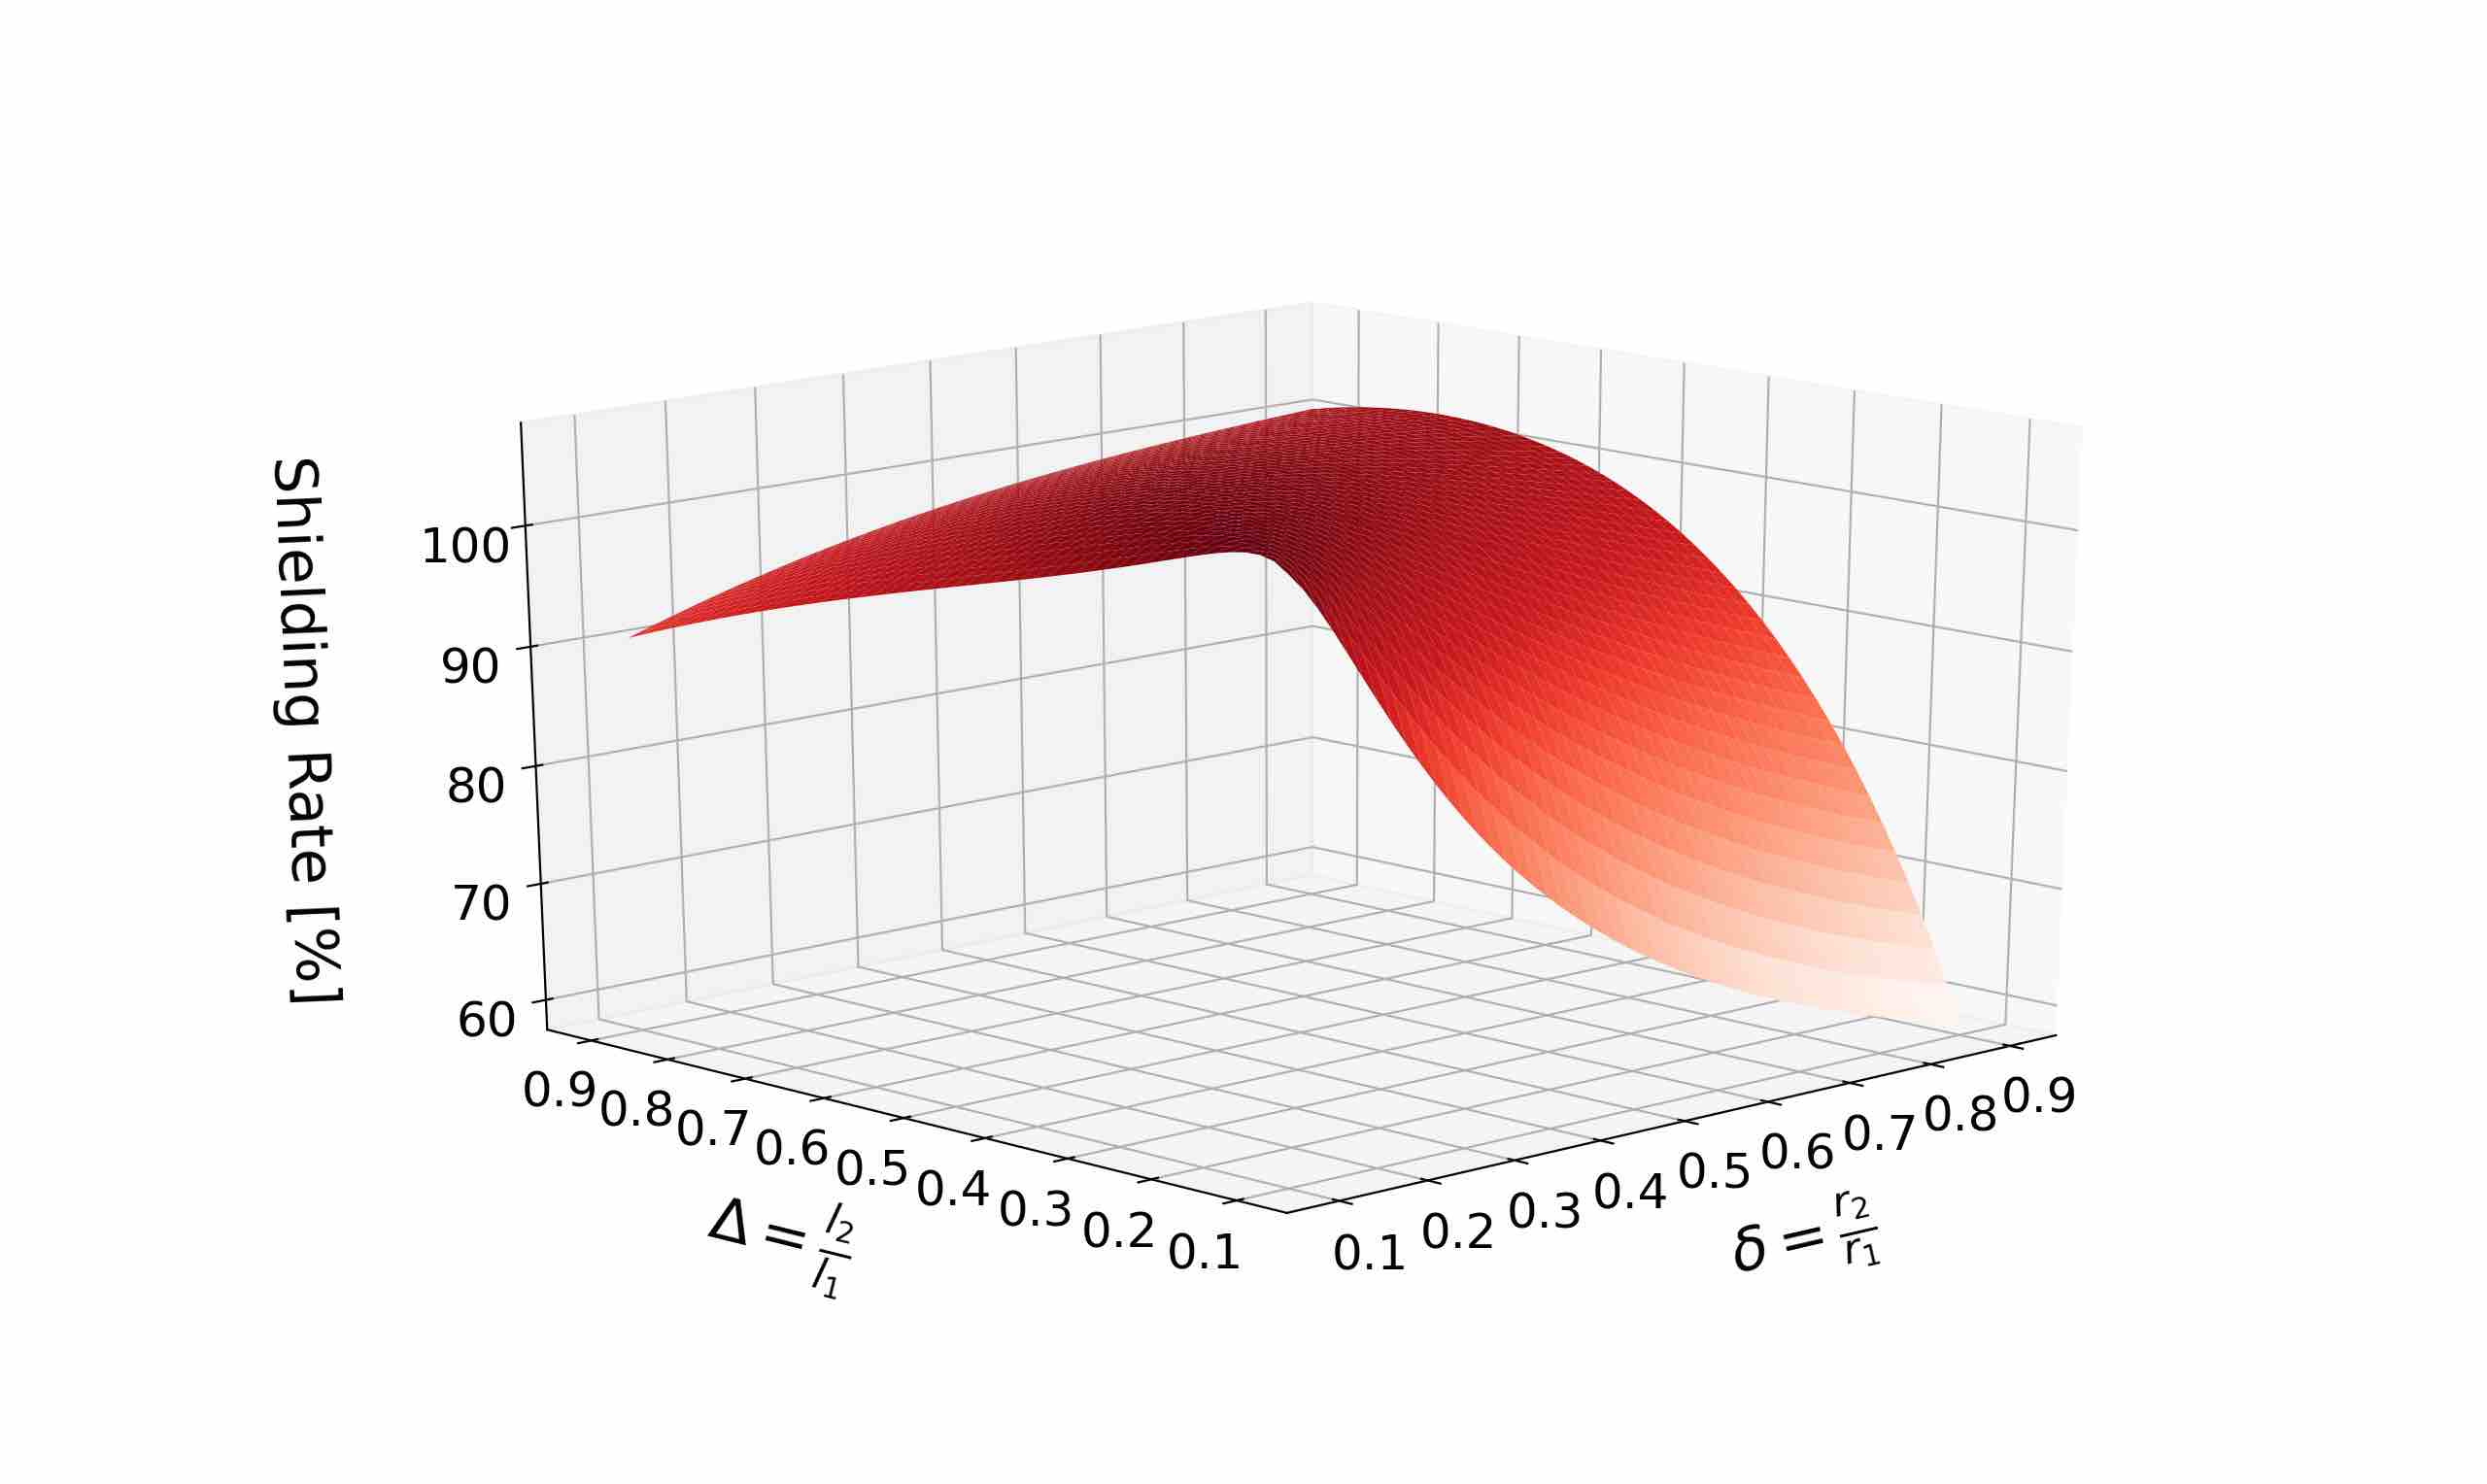
\includegraphics[width=17cm, bb=9 9 900 550]{./section3Effectiveness/simulatedShieldingRates3D1.JPEG}
  \caption{Simulated shielding rates with different $r_2, l_2$.}
  \label{fig:simulatedShieldingRates3D1}
\end{figure}
\begin{figure}[H]
  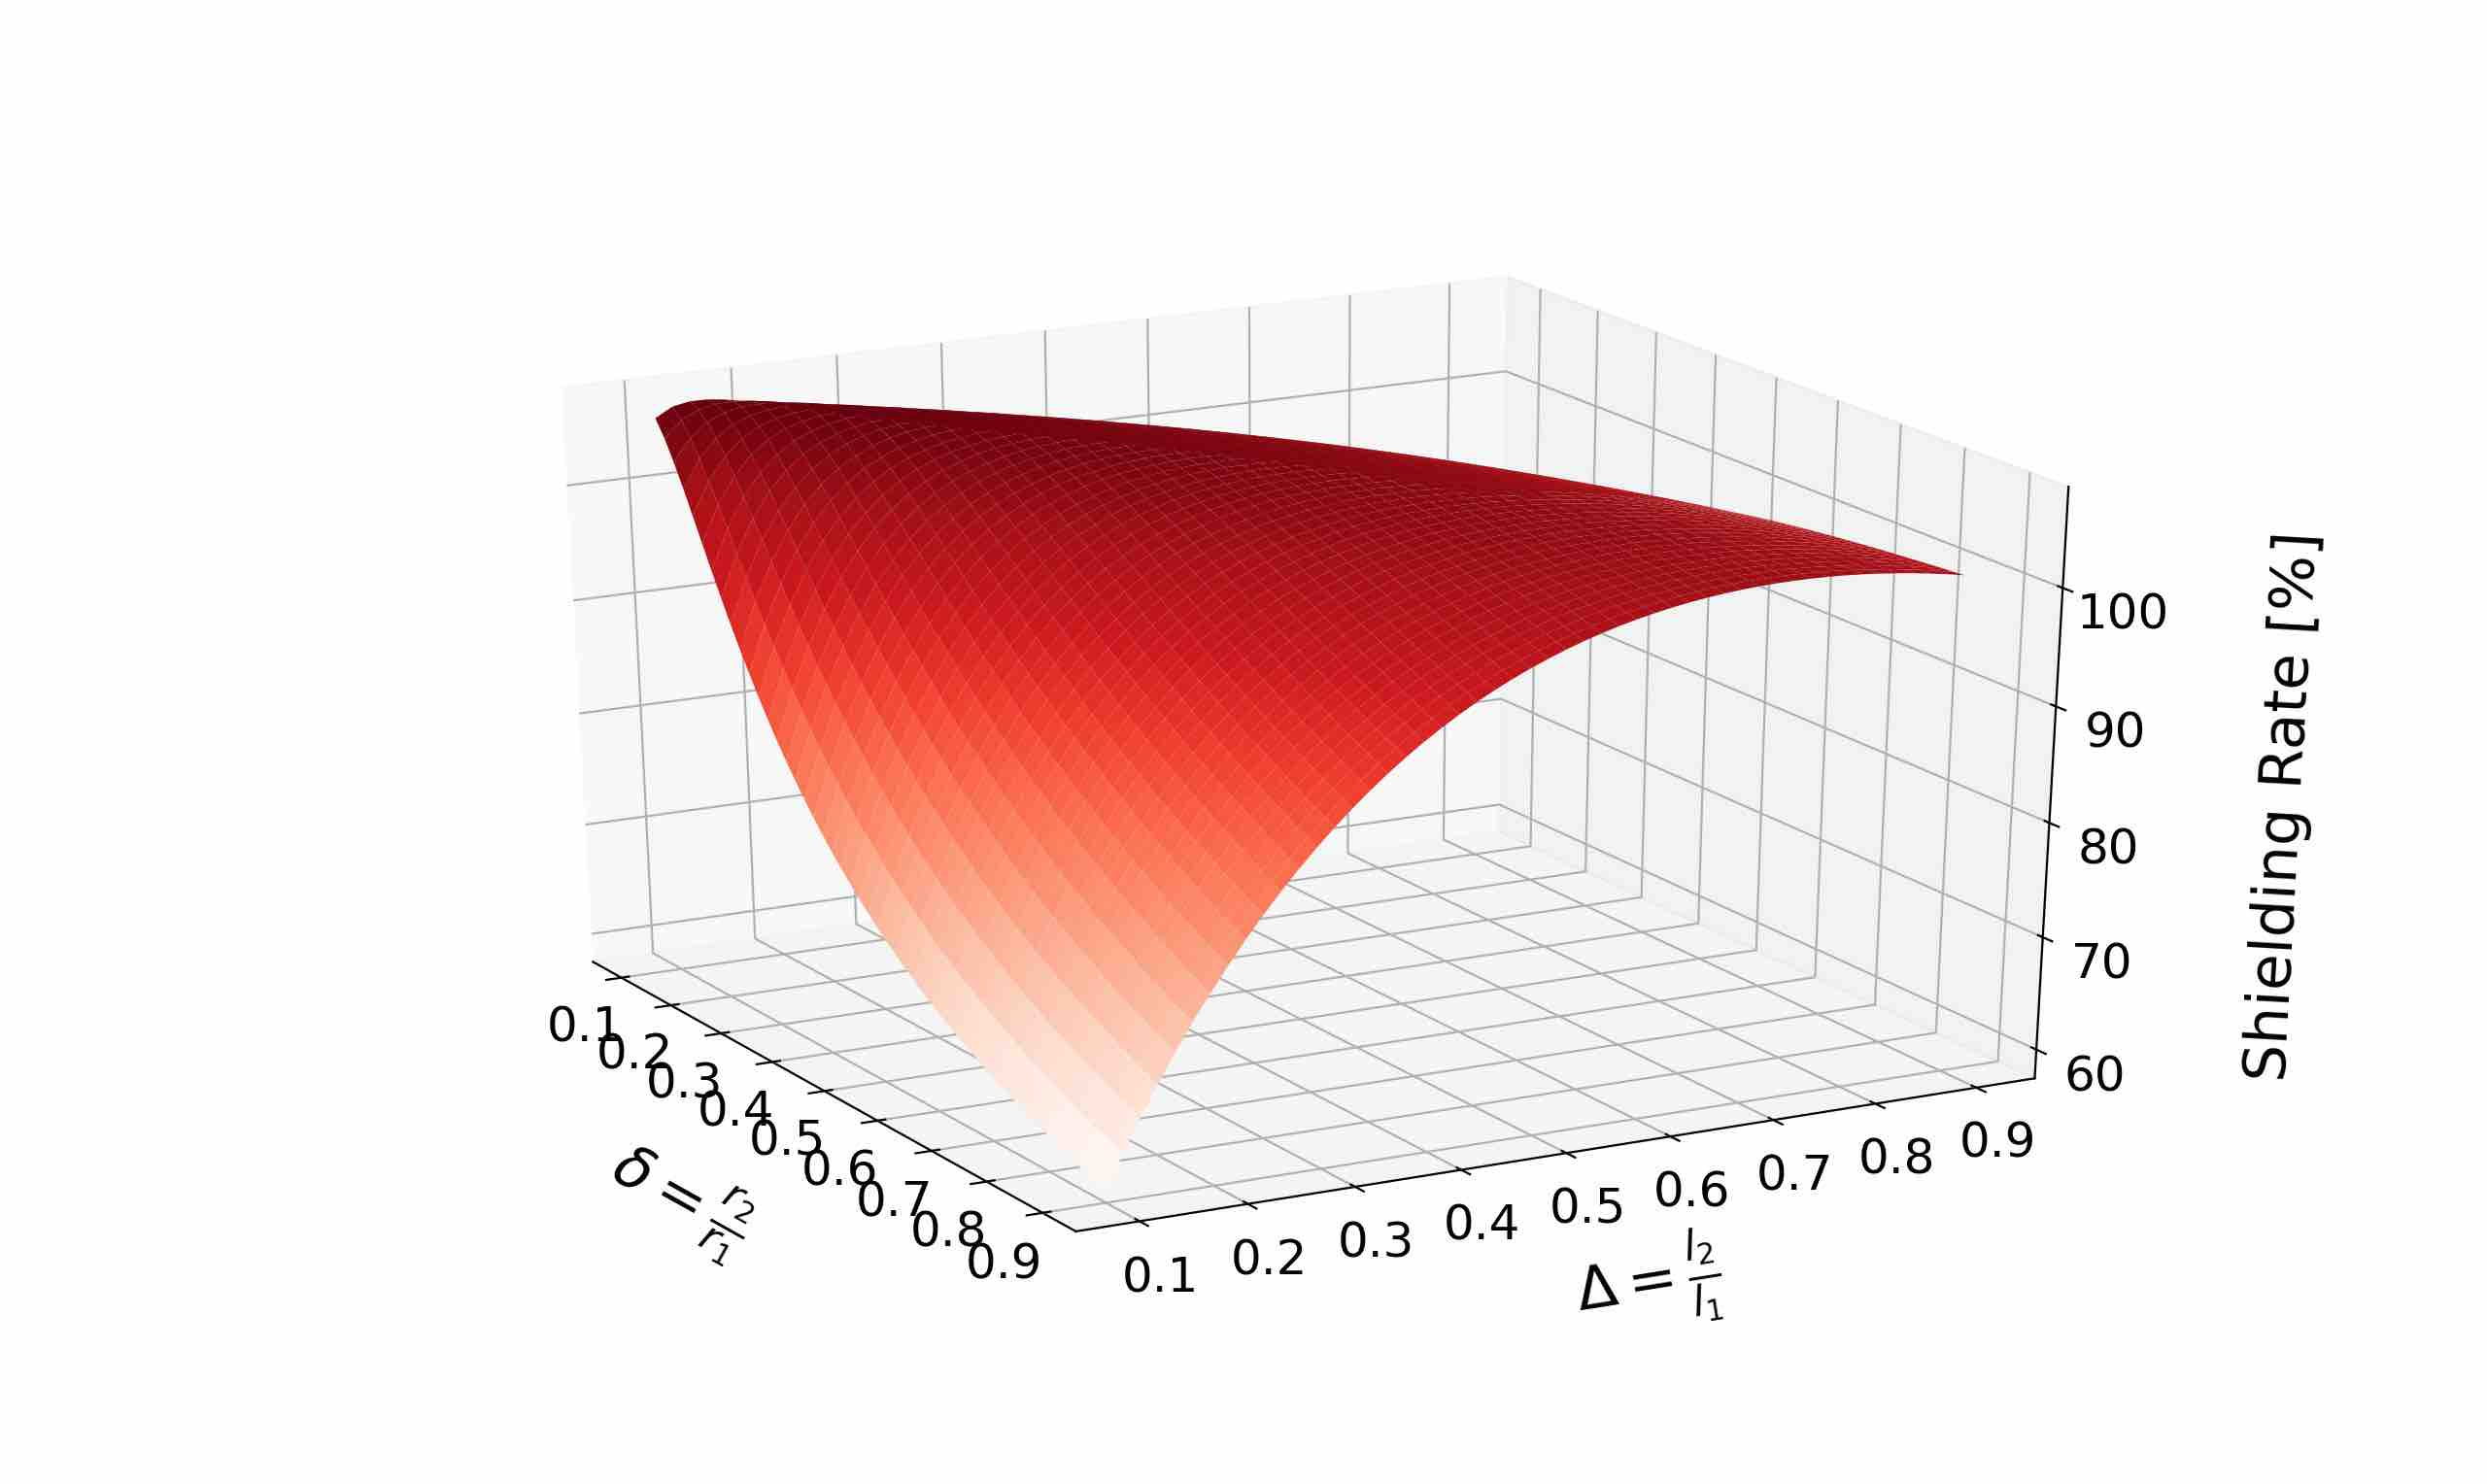
\includegraphics[width=17cm, bb=9 9 900 550]{./section3Effectiveness/simulatedShieldingRates3D2.JPEG}
  \caption{Simulated shielding rates with different $r_2, l_2$.}
  \label{fig:3D2}
\end{figure}
\begin{figure}[H]
  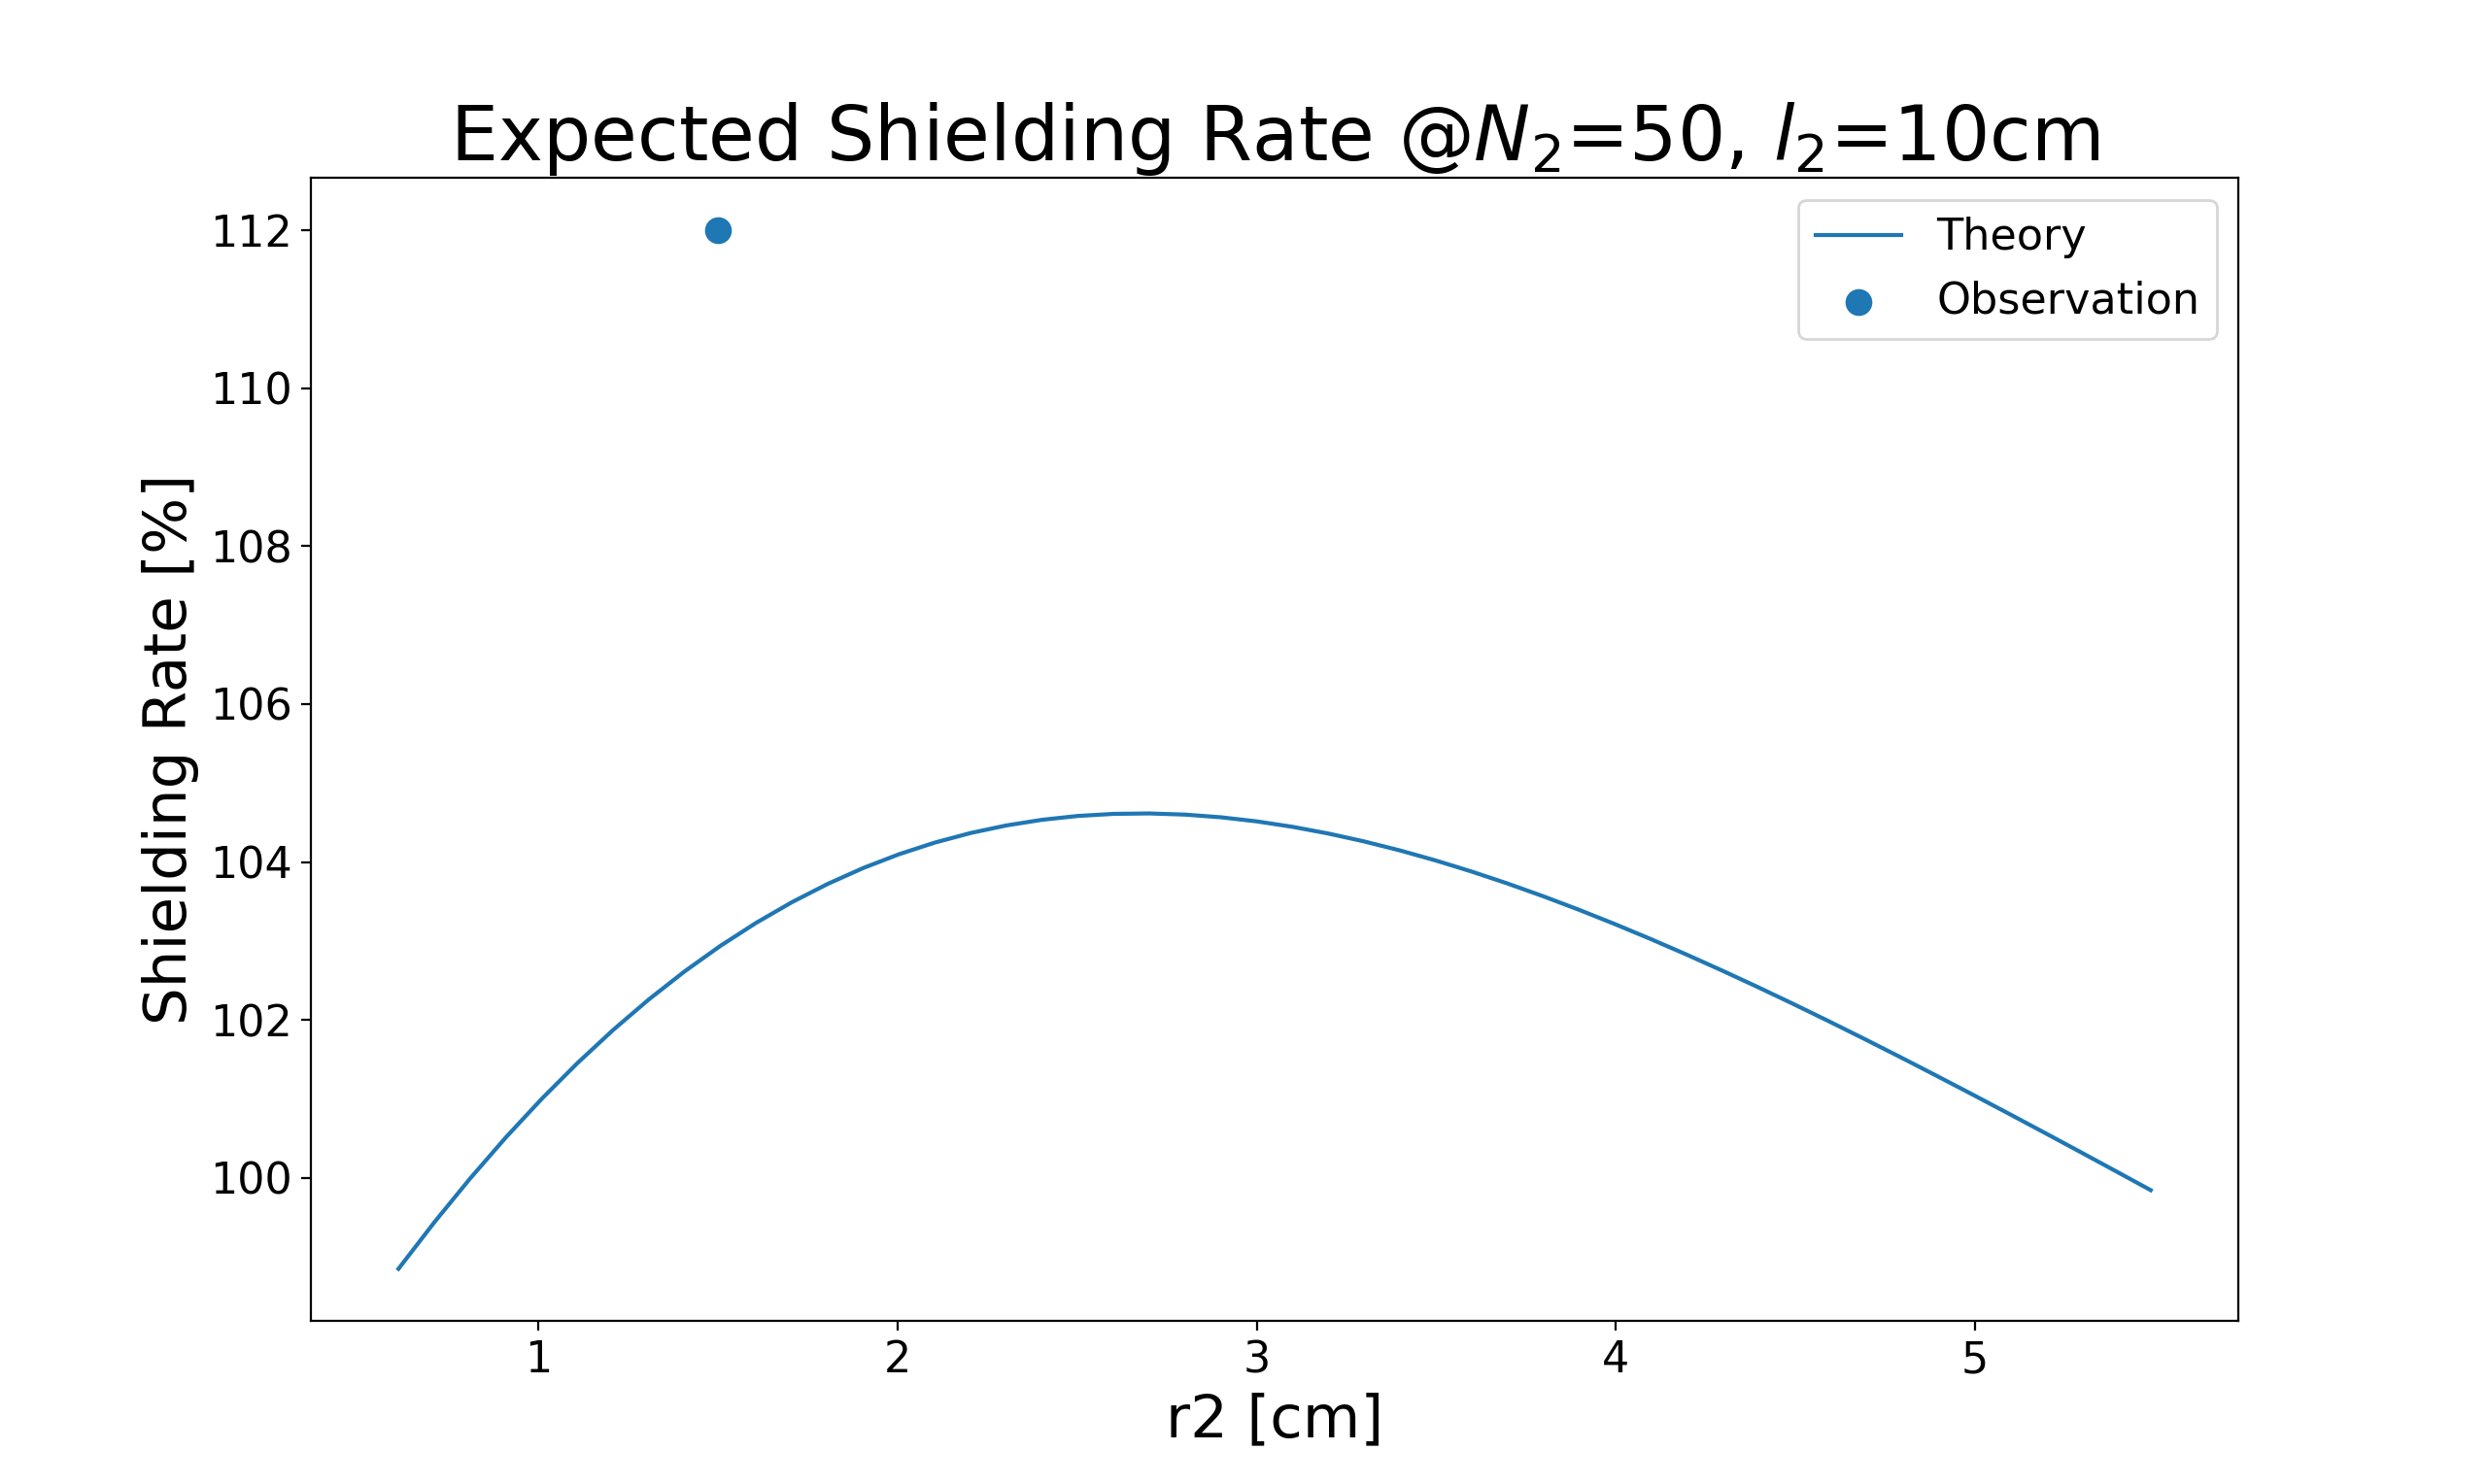
\includegraphics[width=17cm, bb=9 9 900 500]{./section3Effectiveness/simulatedShieldingRates2.png}
  \caption{Simulated and observed shielding rates with fixed $l_2 = 10$[cm], $N_2 = 50$, varied $r_2$.}
  \label{fig:overshielding}
\end{figure}

From Fig. \ref{fig:simulatedShieldingRates3D1} and \ref{fig:simulatedShieldingRates3D2},
2 notable points can be observed:
\begin{enumerate}
  \item As described, to achieve high shielding rates one must have the inner/outer coil aspect ratio falls into the right zone.
  For example, coils with radius ratio $\delta = r_2/r_1 = 0.5$ and length ratio $\Delta = l_2/l_1 = 0.5$ hold a shielding rates near 100\%,
  while coils with radius ratio $\delta = r_2/r_1 = 0.9$ and length ratio $\Delta = l_2/l_1 = 0.1$ only shows a poor performance around 70\%.
  \item It is possible for the central shielding rates to exceed 100\%.
  In Fig. \ref{fig:overshielding}, we have plotted the cross section at $l_2 = 0.5$ and $r_2 = 0.2\sim0.6$ out of Fig. \ref{fig:simulatedShieldingRates3D1} into a 2D diagram.
  In which, the simulated and experimental results both show shielding rates over 100\%.
\end{enumerate}

To explain this overshielding phenomenen, let us focus on how the inner current is induced.
From Faraday's law, electrical fields, or electrical currents if in conductive materials,
will be induced according to the magnetic field time variation ACROSS the surface.
This law is often described as the following equation, in integral form.
\begin{equation}
  \oint_{C} rot\mathbf{E}d\mathbf{r} = -\iint_{S}\frac{\partial B}{\partial t}d\mathbf{S}
\end{equation}
For a solenoid coil, the magnitude of the induced current is decided by the magnetic flux flow through the whole internal space.
Since Faraday's low only requires the magnetic field to balance in the entire internal space,
for some part of the space it is possible that the magnetic field produced by the induced current exceeds the field produced by the imposed current.
Physicists may find it easier to understand by considering the phenomenen resulting from the principle of minimum potential energy.
Engineers can approach from the fact that a solenoid winding generates a denser fields in the centeral part.
Anyway, even though overshielding occurs, as long as the shielding rates wanders around 100\%,
the actual magnetic field approaches zero.


\subsubsection{Method}
To testify the shielding rates, a series of experiments have been conducted useing the equipment introducd in section 3.1.
In this section, since the shielding rate is hard to measured under a DC condition,
we have chosen the imposed currents to be sin waves.
In this way, the induced currents on the internal coil would alse be sin waves,
from which the shielding effects can be measured easily from the magnitude.
To improve the accuracy, we have recorded 100 waves for each point, and measured the magnitude before they were averaged.
The procedure of our experiments is shown as following.
\begin{enumerate}
  \item Set the internal superconductor coil, and coil by liquid Nitrogen.
  \item Impose sin wave current continuously at specific magnitude and frequency.
  \item Measure the magnetic field variation in time domain, until data containing 100 wave lengths long are recorded.
  \item Transfer the measured magnetic field data into frequency domain data using fourier transform module provided by numpy.
  \item Take the magnitude at the certain imposed frequency and devided by the coefficient of the hall sensor,
  which is $89.34$ [$\mu$V/mT] in our experiments,
  to transfer the voltage data into $B$ field data.
  (Ensure the magnitude should be the maximum among the frequency domain data).
  This is taken as the measured $B$ field with shielding, at the certain position.
  \item If the $B$ field data along certain axis is need, then move to the next position and repeat from step 1.
  \item After the $B$ fields with shielding are recorded, remove the internal superconductor coil,
  and measure the $B$ fields along the same positions.
  Theese are taken as the measured $B$ field without shielding.
  Note that through the entire measuring experiments, the equipment is soaked in liquid Nitrogen.
\end{enumerate}
A 2 turn superconductive solenoid coil is used as the internal coil, while the external copper coil remains the same.
Parameters of this experiment is shown in Tab. \ref{tab:shieldingRateExpParameters}
\begin{table}[H]
  \centering
  \caption{Specification and parameters used in the shielding experiment.}
  \label{tab:shieldingRateExpParameters}
  \begin{tabular}{cccc}\hline\hline
    Parameter & Internal Coil1 & External Coil \\
    Diameter [cm] & 3.0 & 14\\
    Length [cm] & 10 & 20 \\
    Turns & 50 & 40 \\
    Critical Current $I_C$ [A] & 30 & Copper \\
    Width of Superconductor Tape & 12 & -\\\hline\hline
  \end{tabular}
\end{table}


\subsubsection{Result and Discussion}
The result of shielding rate measurement along the z axis is shown in Fig. \ref{fig:shieldingAbilityMeasuredBs}, and Fig. \ref{fig:shieldingAbilityMeasuredShieldingRates}.

\begin{figure}[H]
  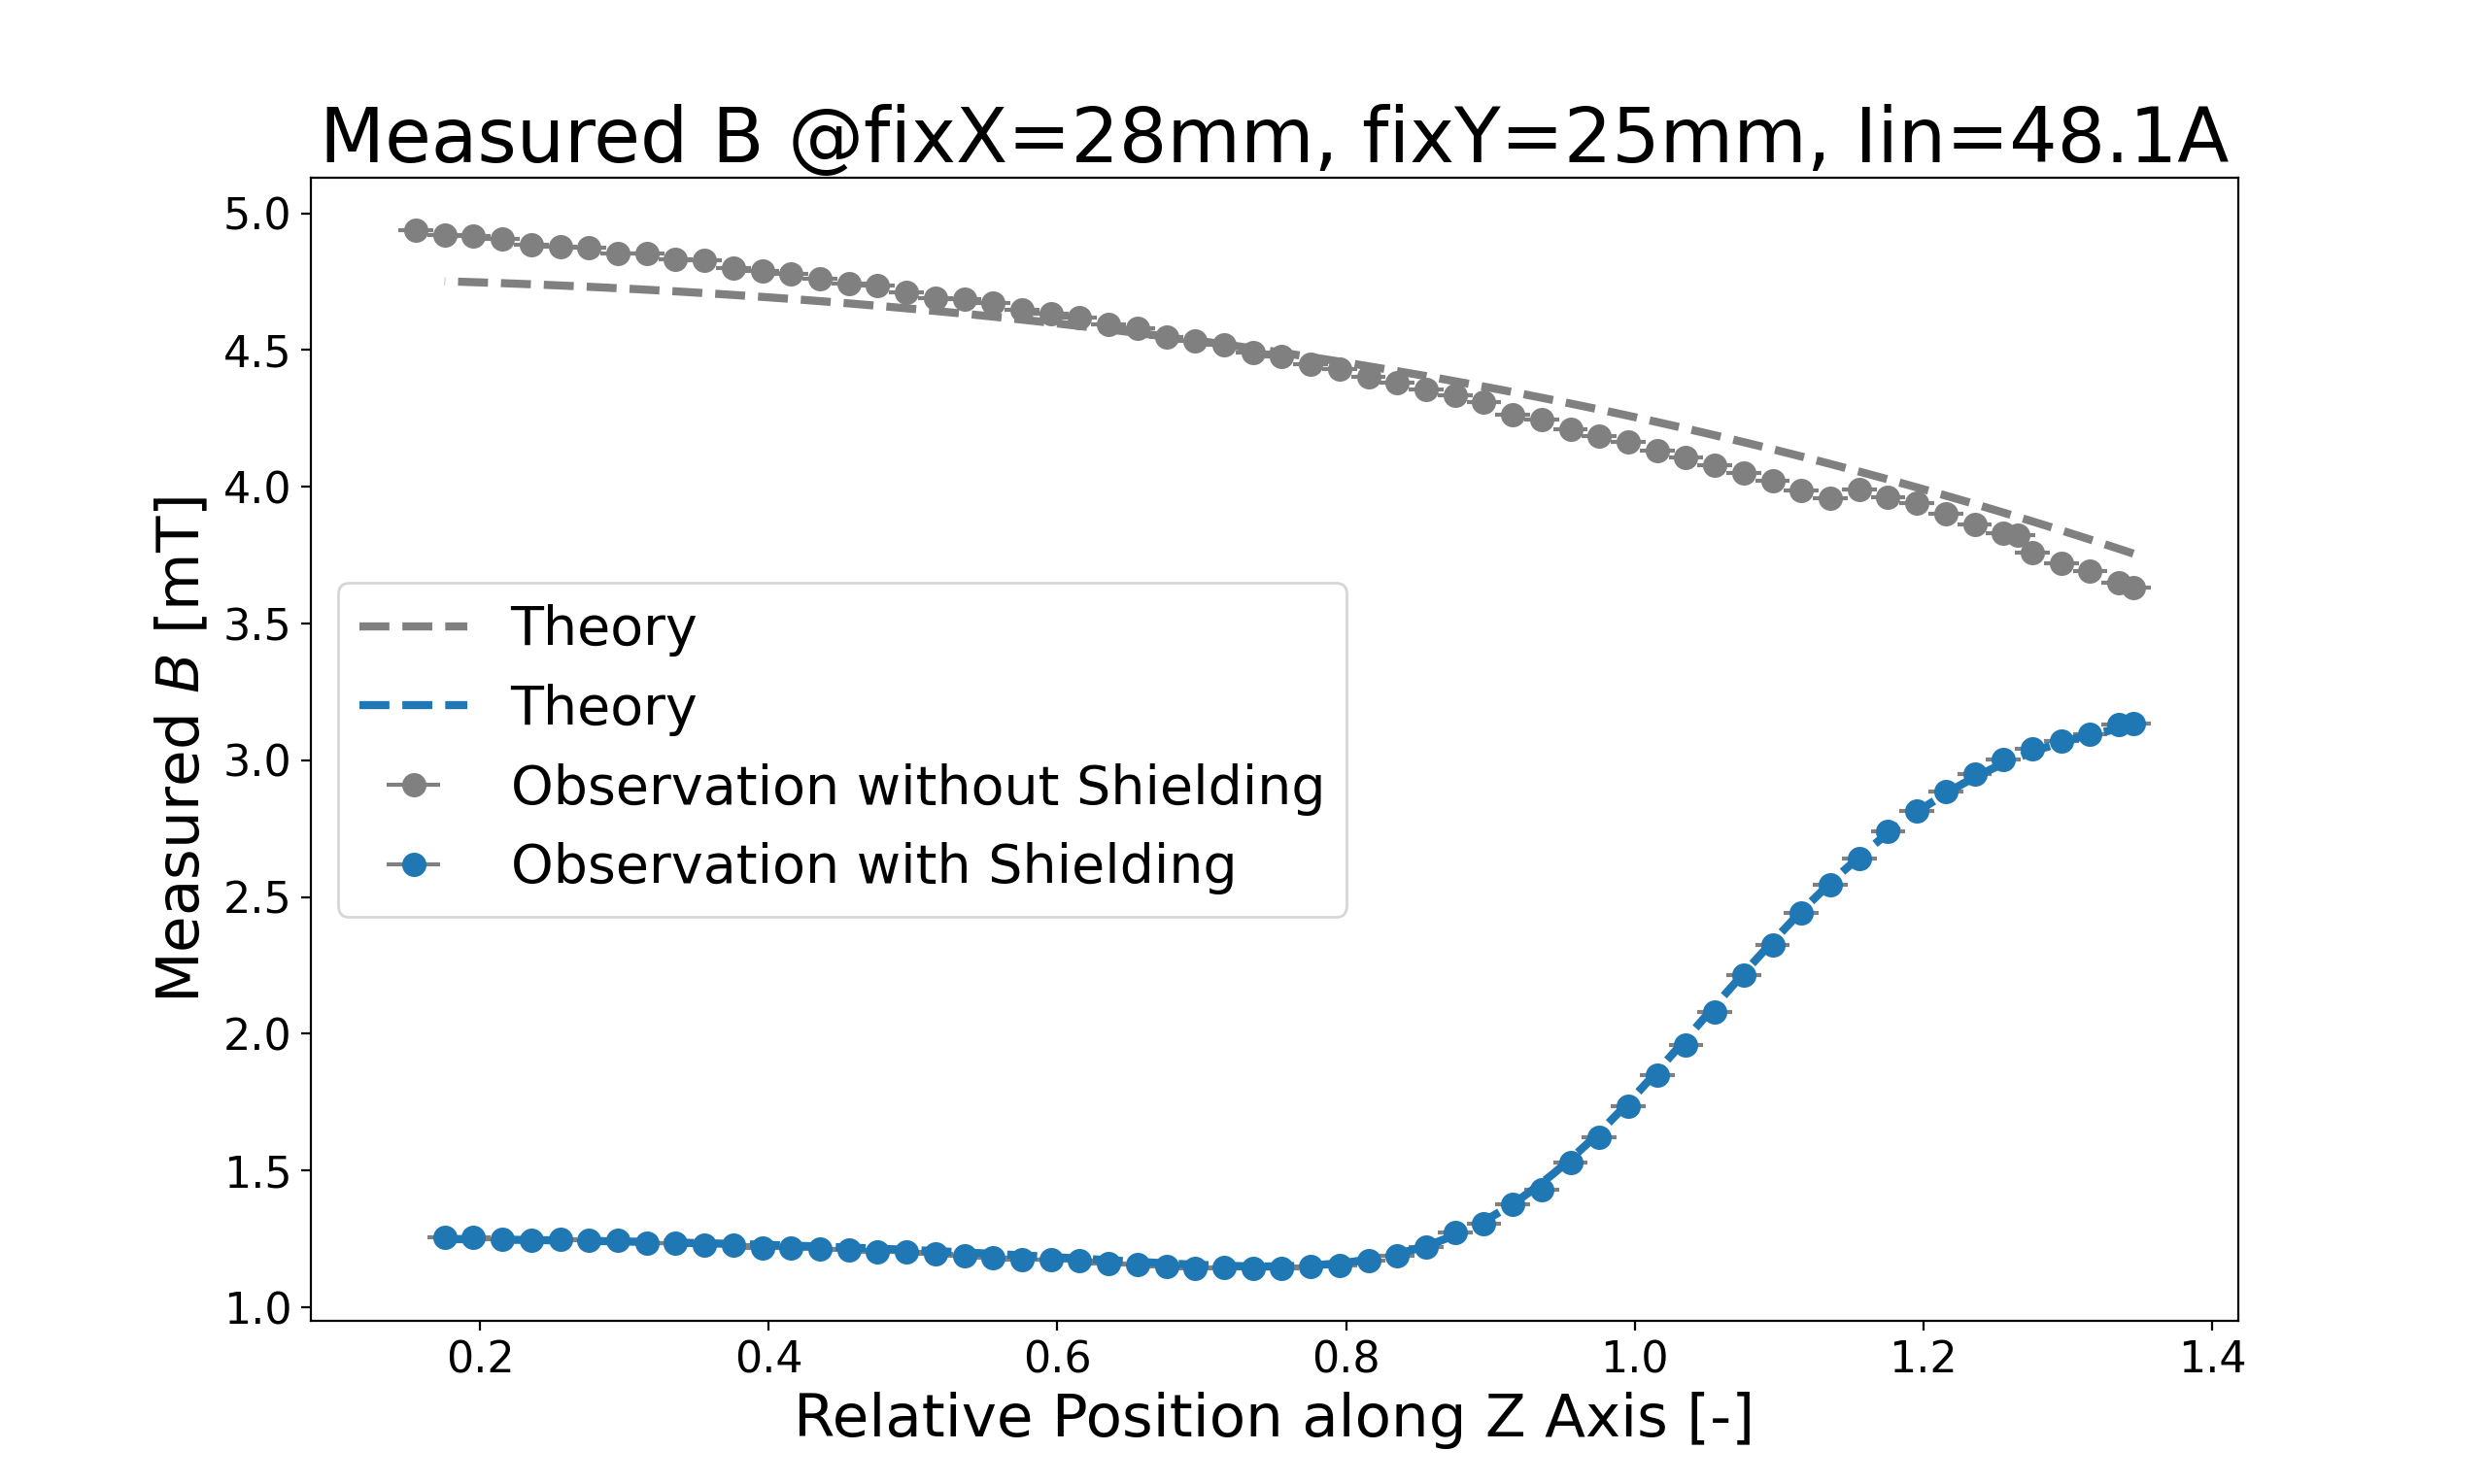
\includegraphics[width=17cm, bb=9 9 900 520]{./section3Effectiveness/measuredBsSolenoid.png}
  \caption{Measured magnitude $\mathrm{abs}(B)$ along the Z axis.}
  \label{fig:shieldingAbilityMeasuredBs}
\end{figure}
\begin{figure}[H]
  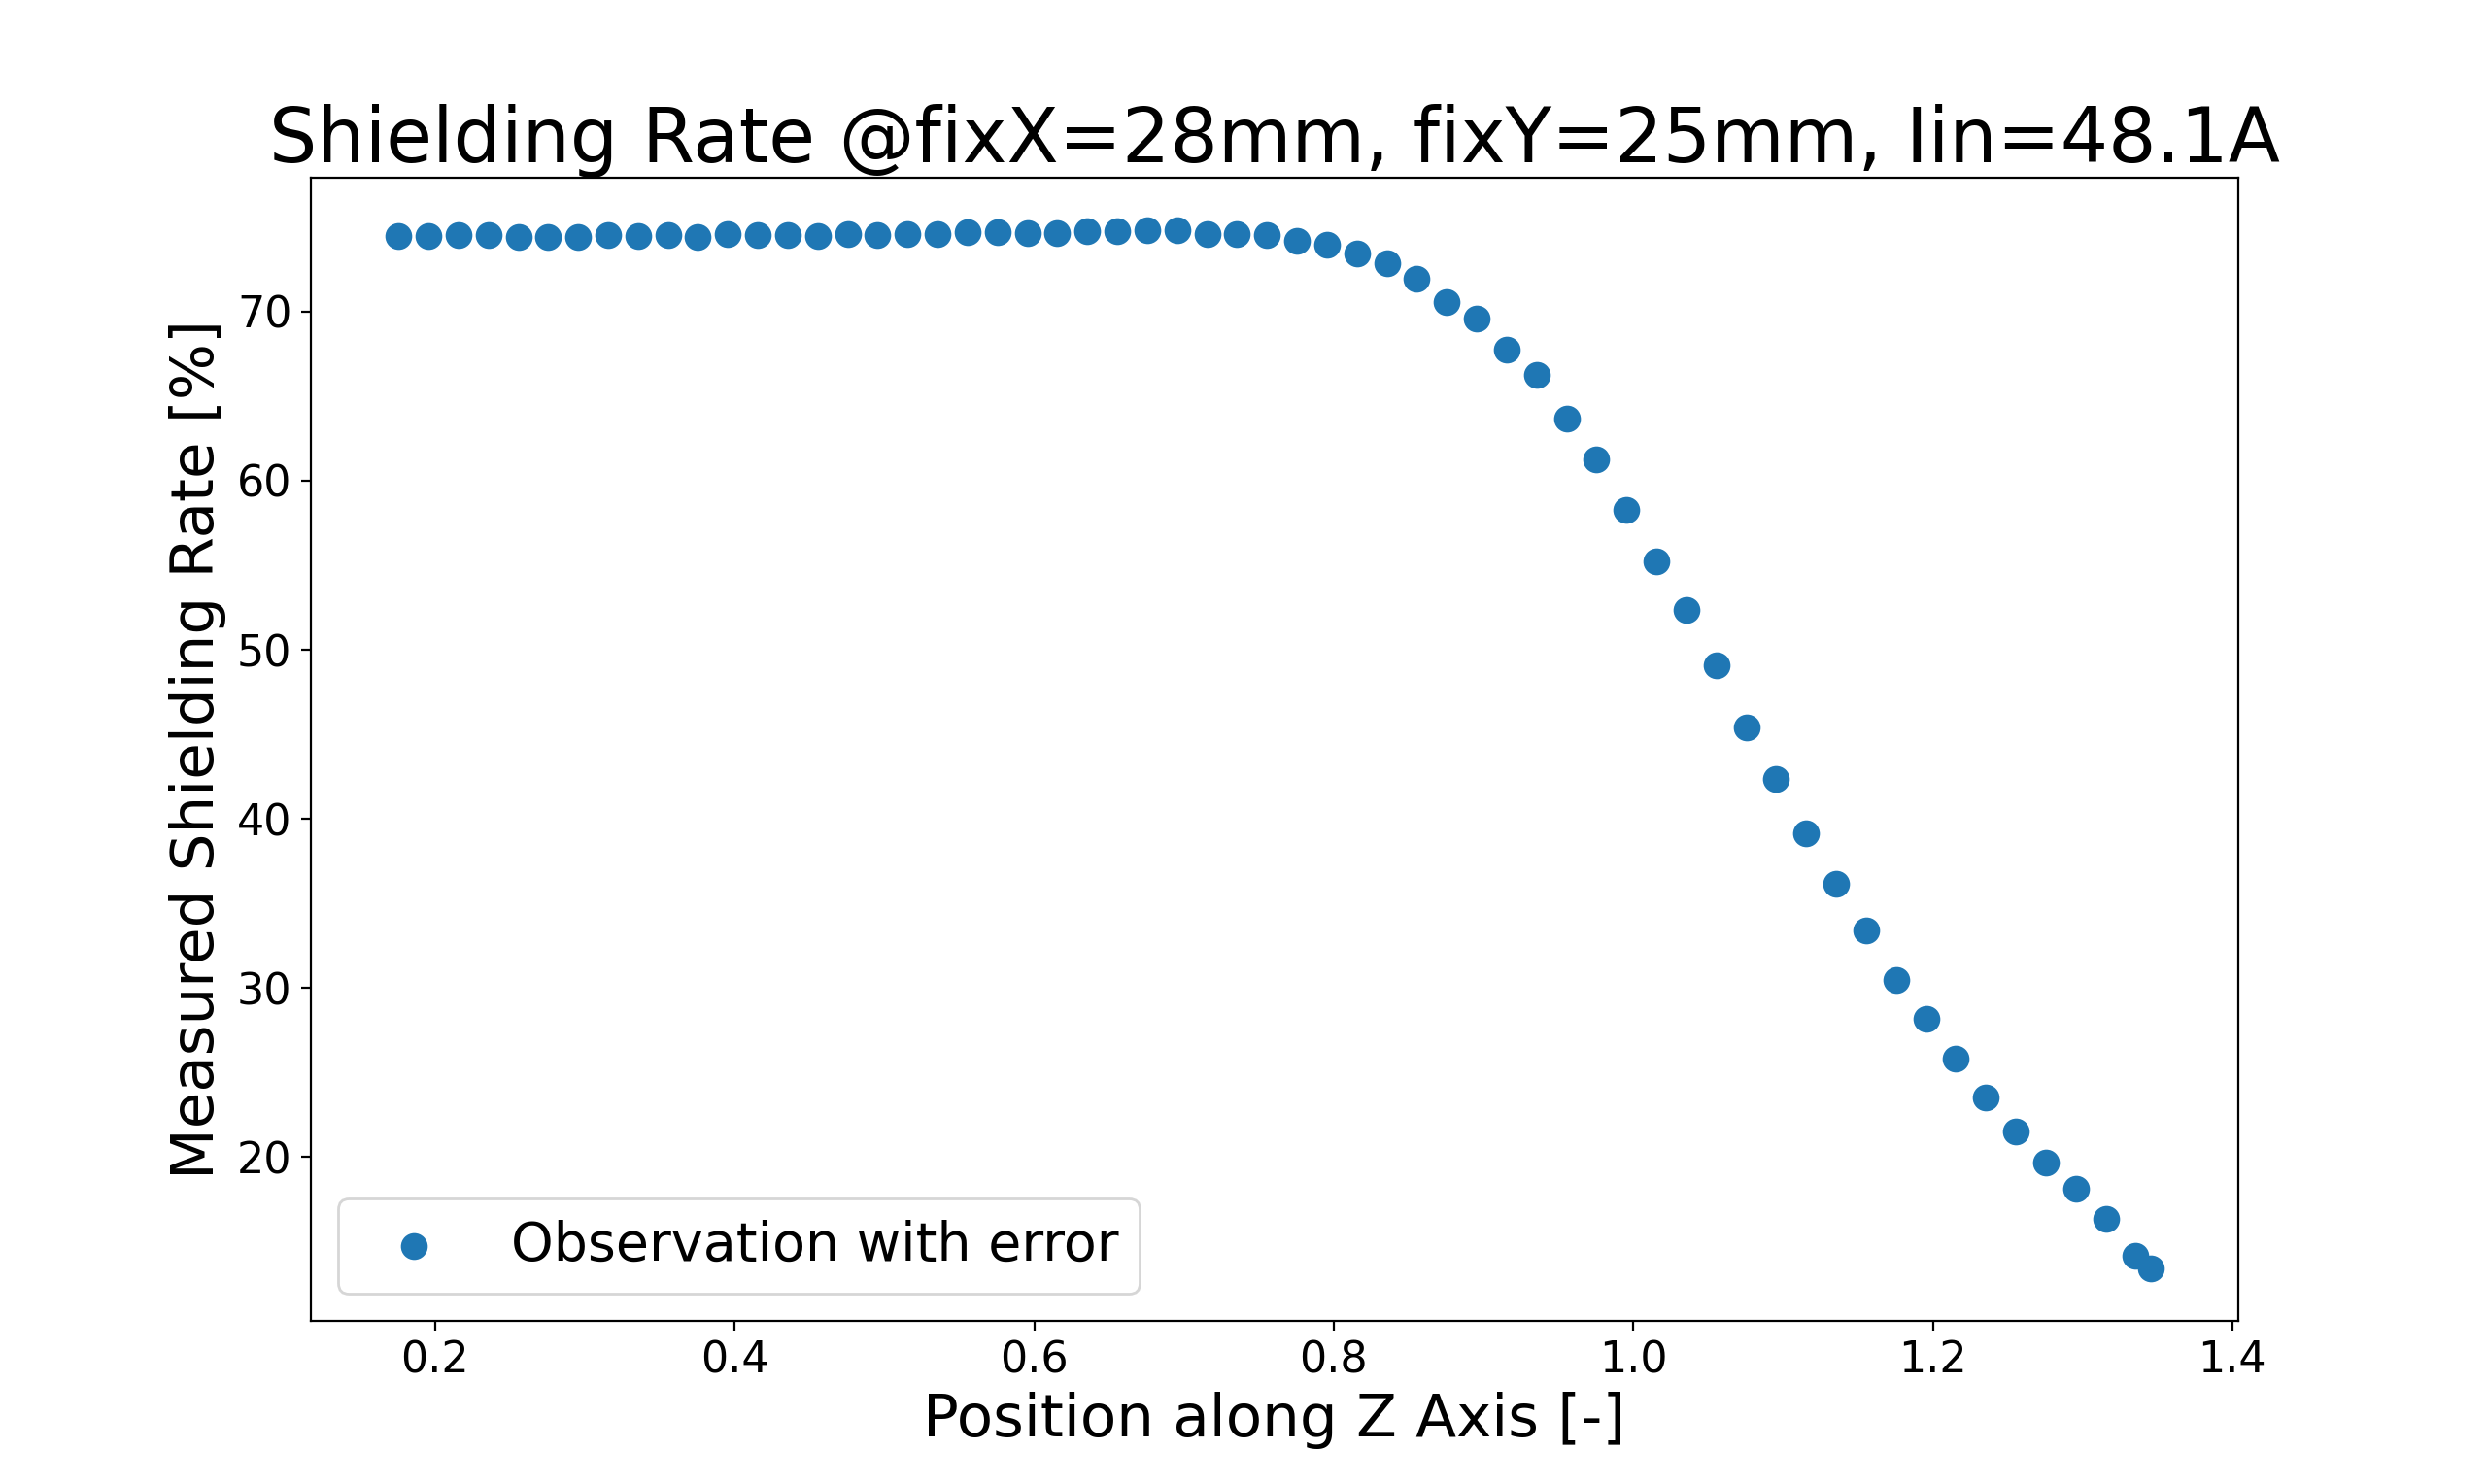
\includegraphics[width=17cm, bb=9 9 900 480]{./section3Effectiveness/measuredShieldingRatesSolenoid.png}
  \caption{The measured shielding rate and the expected shielding rates under ideal condition. The solid points are evaluated by $(1-B_{measured}/B_{imposed})$ directly from Fig.\ref{fig:measuredBSolenoid}, while the transparent points are evaluated by equation (4), along with the theoretical line.}
  \label{fig:shieldingAbilityMeasuredShieldingRates}
\end{figure}
In Fig. \ref{fig:shieldingAbilityMeasuredShieldingRates},
the solid points represent the measured $B$ fields along the z axis.
From which, the shielding rate reaches around 78\% inside the internal coil.
The outer the position gets, the lower the shielding rate goes.

The maximum shielding rate 78\% may seem low.
This is due to the coil being small, with low inductance and relatively high resistance.
According to equation (30) or (35), the shielding rate should be no concern with the impedance including $\omega L$ and $R$,
as shown below.
\begin{eqnarray}
  B(t) &=& C_1\cdot i_1(t) - C_2\cdot i_2(t)\nonumber\\
  &|& C_1 = \sum_{i=1}^{N1} \frac{\mu_0r_1^2}{2\left(r_1^2 + d_i^2\right)^{\frac{3}{2}}} \in \mathrm{constant}\nonumber\\
  &|& C_2 = \sum_{i=1}^{N2} \frac{\mu_0r_2^2}{2\left(r_2^2 + d_i^2\right)^{\frac{3}{2}}} \in \mathrm{constant}\nonumber\\
  &|& i_1(t) = I_1\sin(\omega t)\nonumber\\
  &|& i_2(t) = \frac{M}{L_2}I_1\sin(\omega t)\nonumber\\
  &=& \left(C_1I_1 - C_2\frac{MI_1}{L_2}\right)\sin(\omega t)|\omega L_2 \gg R_2\\
  Shielding Rate &=& \frac{C_2\cdot i_2(t)}{C1\cdot i_1(t)} = \frac{C_2}{C_1}\cdot\frac{M}{L_2}
\end{eqnarray}
However, if the $\omega L_2 \ll R_2$ doesn't hold, which means the resistance of the internal coil is not neglectable,
the induced current would become
\begin{eqnarray}
  i_2(t) &=& \frac{j\omega M}{j\omega L_2 + R_2}\cdot I_1\sin(\omega t)\nonumber\\
  &=& \frac{1}{\sqrt{1+\left(\frac{R_2}{\omega L_2}\right)^2}}\cdot \frac{M}{L_2}I_1\sin(\omega t + \theta)\\
  &|& \theta = \tan^{-1}(\frac{R_2}{\omega L_2})\nonumber
\end{eqnarray}
where $j$ denotes the imaginary unit, $M$ denote the mutual inductance of the inner-outer coils,
$L_2$ denotes the inductance of the inner coil.
Mark that the transient term is emitted here for convenience.
With equation (39), it is obvious that the magnitude of the induced current $i_2(t)$ is multiplied by
$\frac{1}{\sqrt{1+(\omega L_2)^2}} < 1$ and the phase of which is delayed by $\theta > 0$,
which indicates a weaker induce current as well as a weaker magnetic shielding ability.
Accordingly, the magnetic field $B$ distribution along Z axis can be denoted as equation (40) and the shielding rate can be derived to be equation (41).
\begin{eqnarray}
  B(t) &=& C_1I_1\sin(\omega t) - \frac{C_2}{\sqrt{1+\left(\frac{R_2}{\omega L_2}\right)^2}}\cdot \frac{M}{L_2}I_1\sin(\omega t + \theta)\nonumber\\
  &|& \theta = \tan^{-1}(\frac{R_2}{\omega L_2})\nonumber\\
  &=& \sqrt{a^2 - 2ab\cos(\theta) + b^2}\cdot\sin(\omega t - \phi)\\
  &|& \phi = \tan^{-1}\left(\frac{b\sin(\theta)}{a-b\cos(\theta)}\right)\nonumber\\
  &|& a = C_1I_1 \in \mathrm{constant}\nonumber\\
  &|& b = \frac{M/L_2}{\sqrt{1+\left(\frac{R_2}{\omega L_2}\right)^2}}C_2I_1 \in \mathrm{constant}\nonumber
\end{eqnarray}
\begin{eqnarray}
  Shielding Rate = \frac{C_2}{C_1}\cdot\frac{M}{L_2} = \frac{b}{a}\cdot\sqrt{1+\tan^2\left(\theta\right)}
\end{eqnarray}
The parameter $a, b, \theta, \phi$ in equation (39), (40) can be measured directly, from which the shielding rate can be evaluated.
For instance, example plots of equation (40) with different $\theta$, namely, different $\omega L_2$ and $R_2$,
are shown in Fig.\ref{fig:0.1theta} and Fig.\ref{fig:14theta}
\begin{figure}[H]
  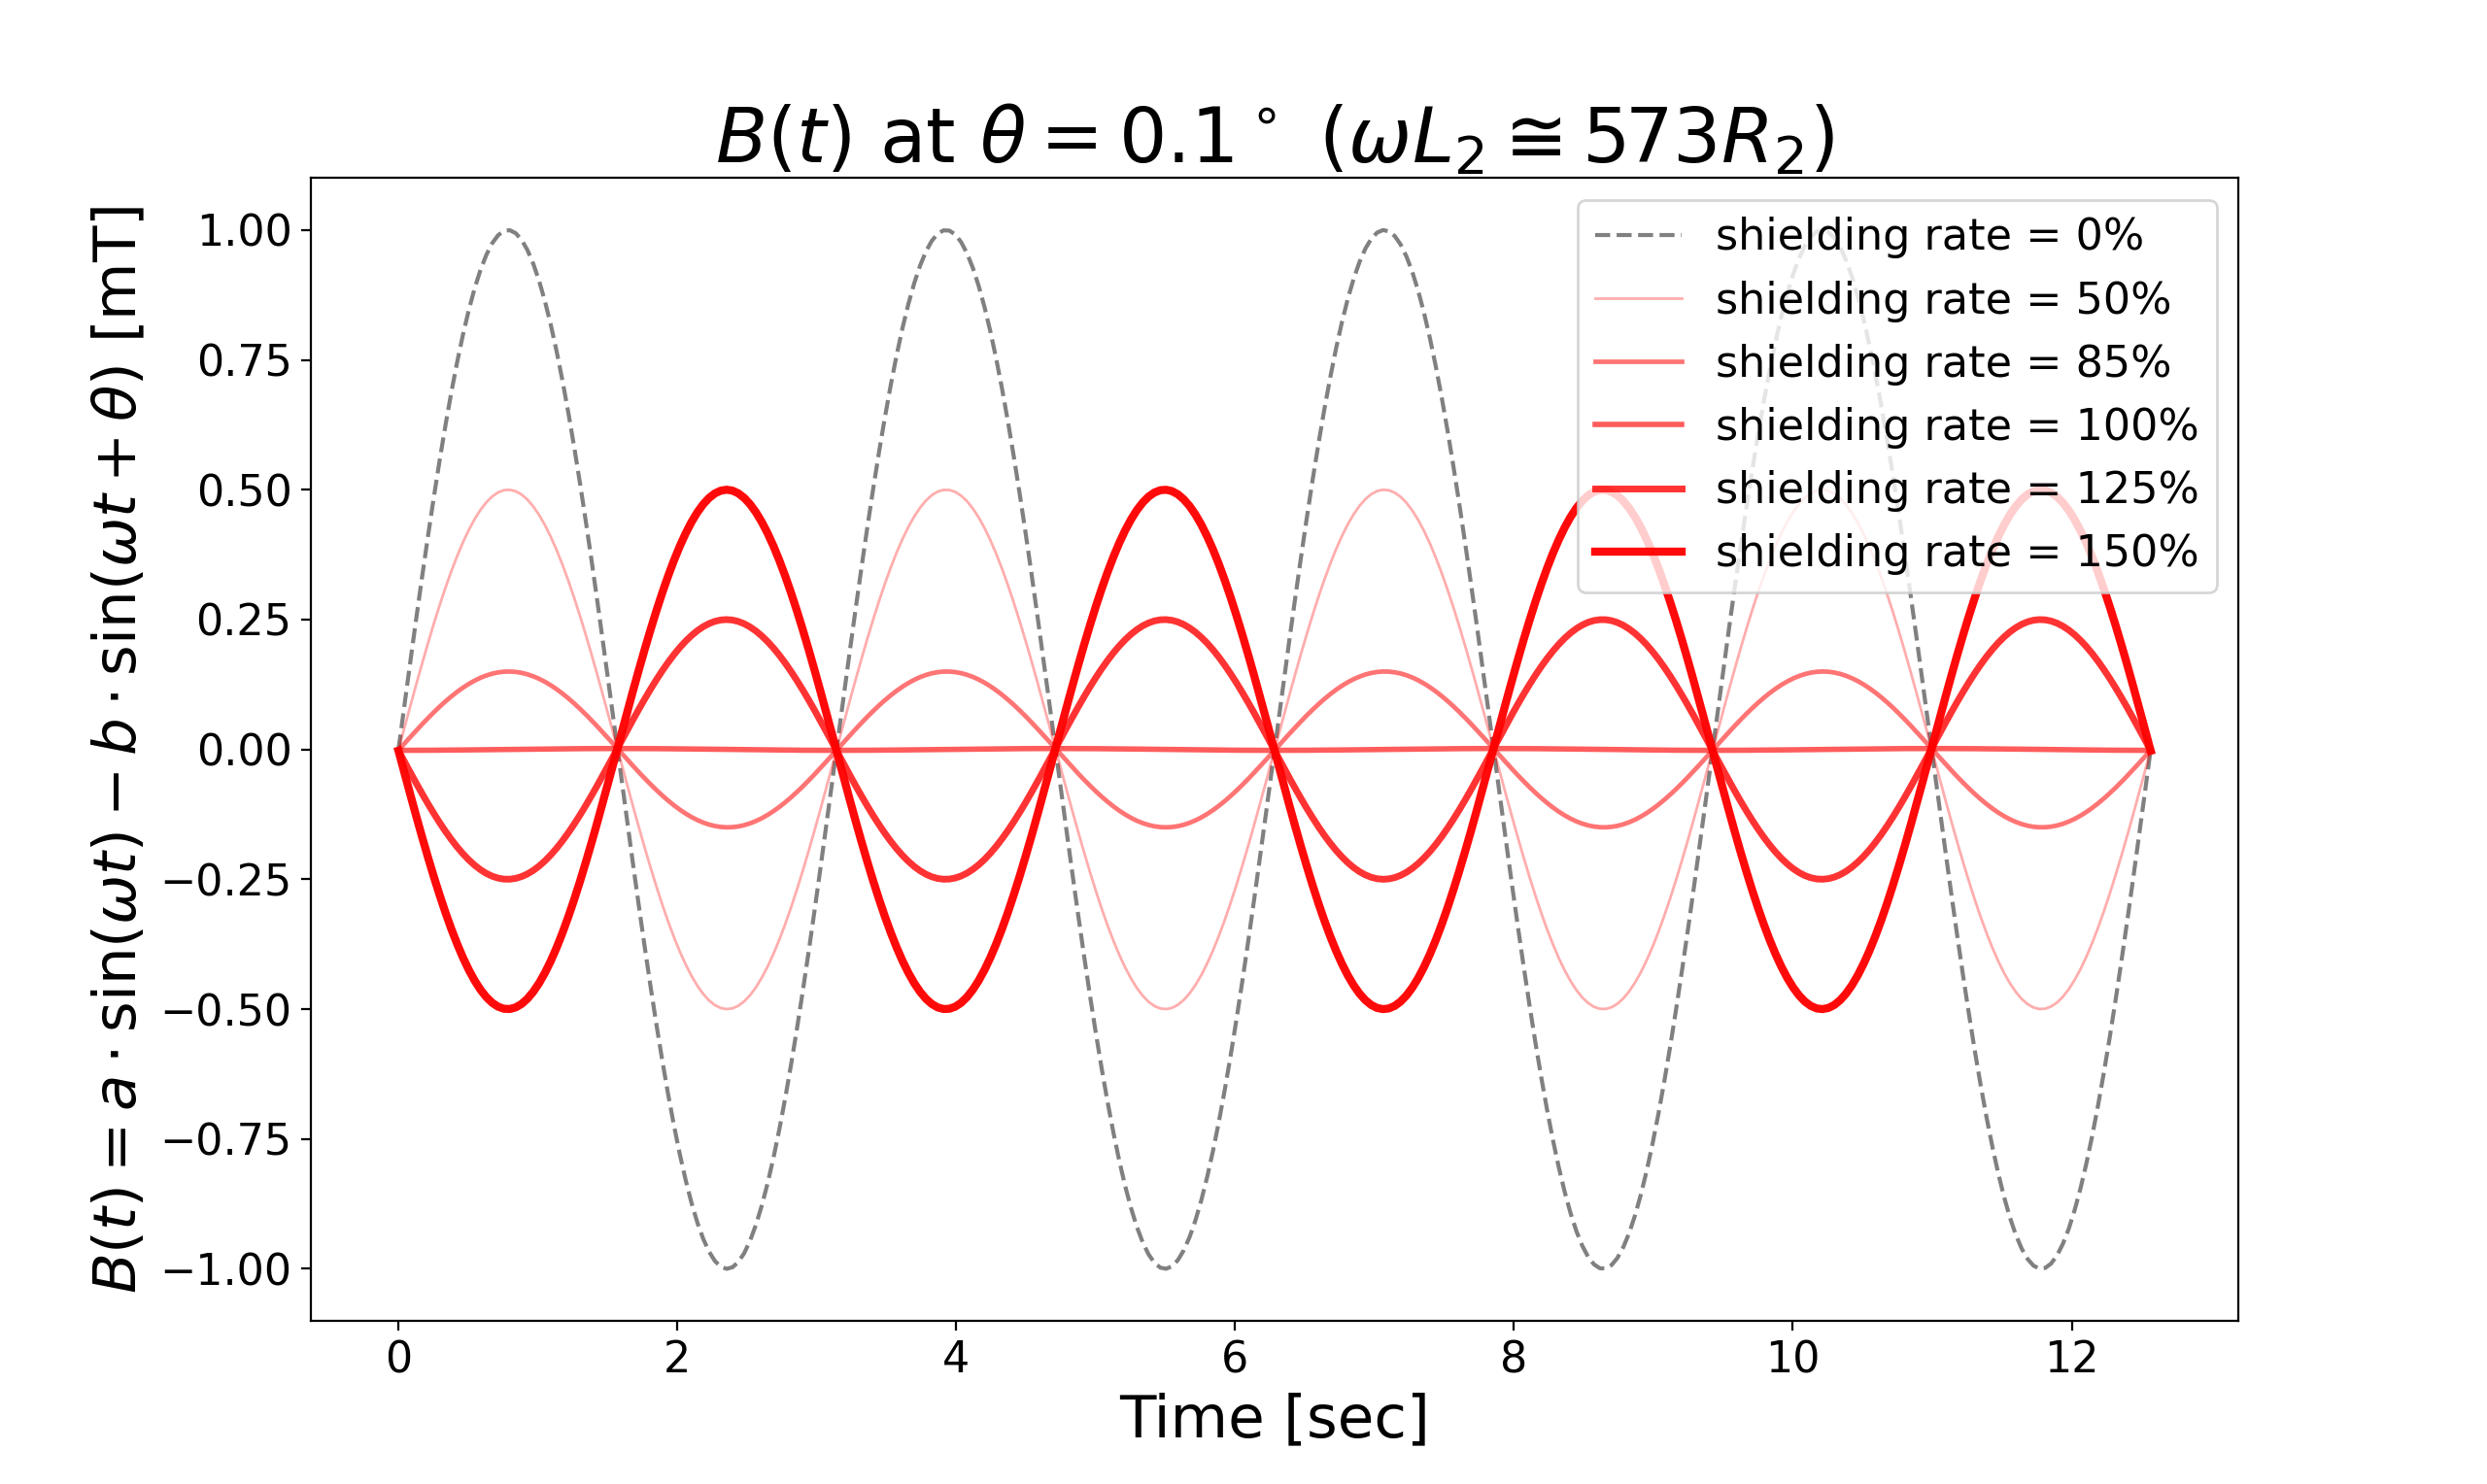
\includegraphics[width=17cm, bb=9 9 900 550]{./section3Effectiveness/sinTestAt0.1deg.png}
  \caption{Simulated $B$ using equation (40) with $\theta = 0.1^\circ$ ($\omega L_2 \cong 573R_2$).}
  \label{fig:0.1theta}
\end{figure}
\begin{figure}[H]
  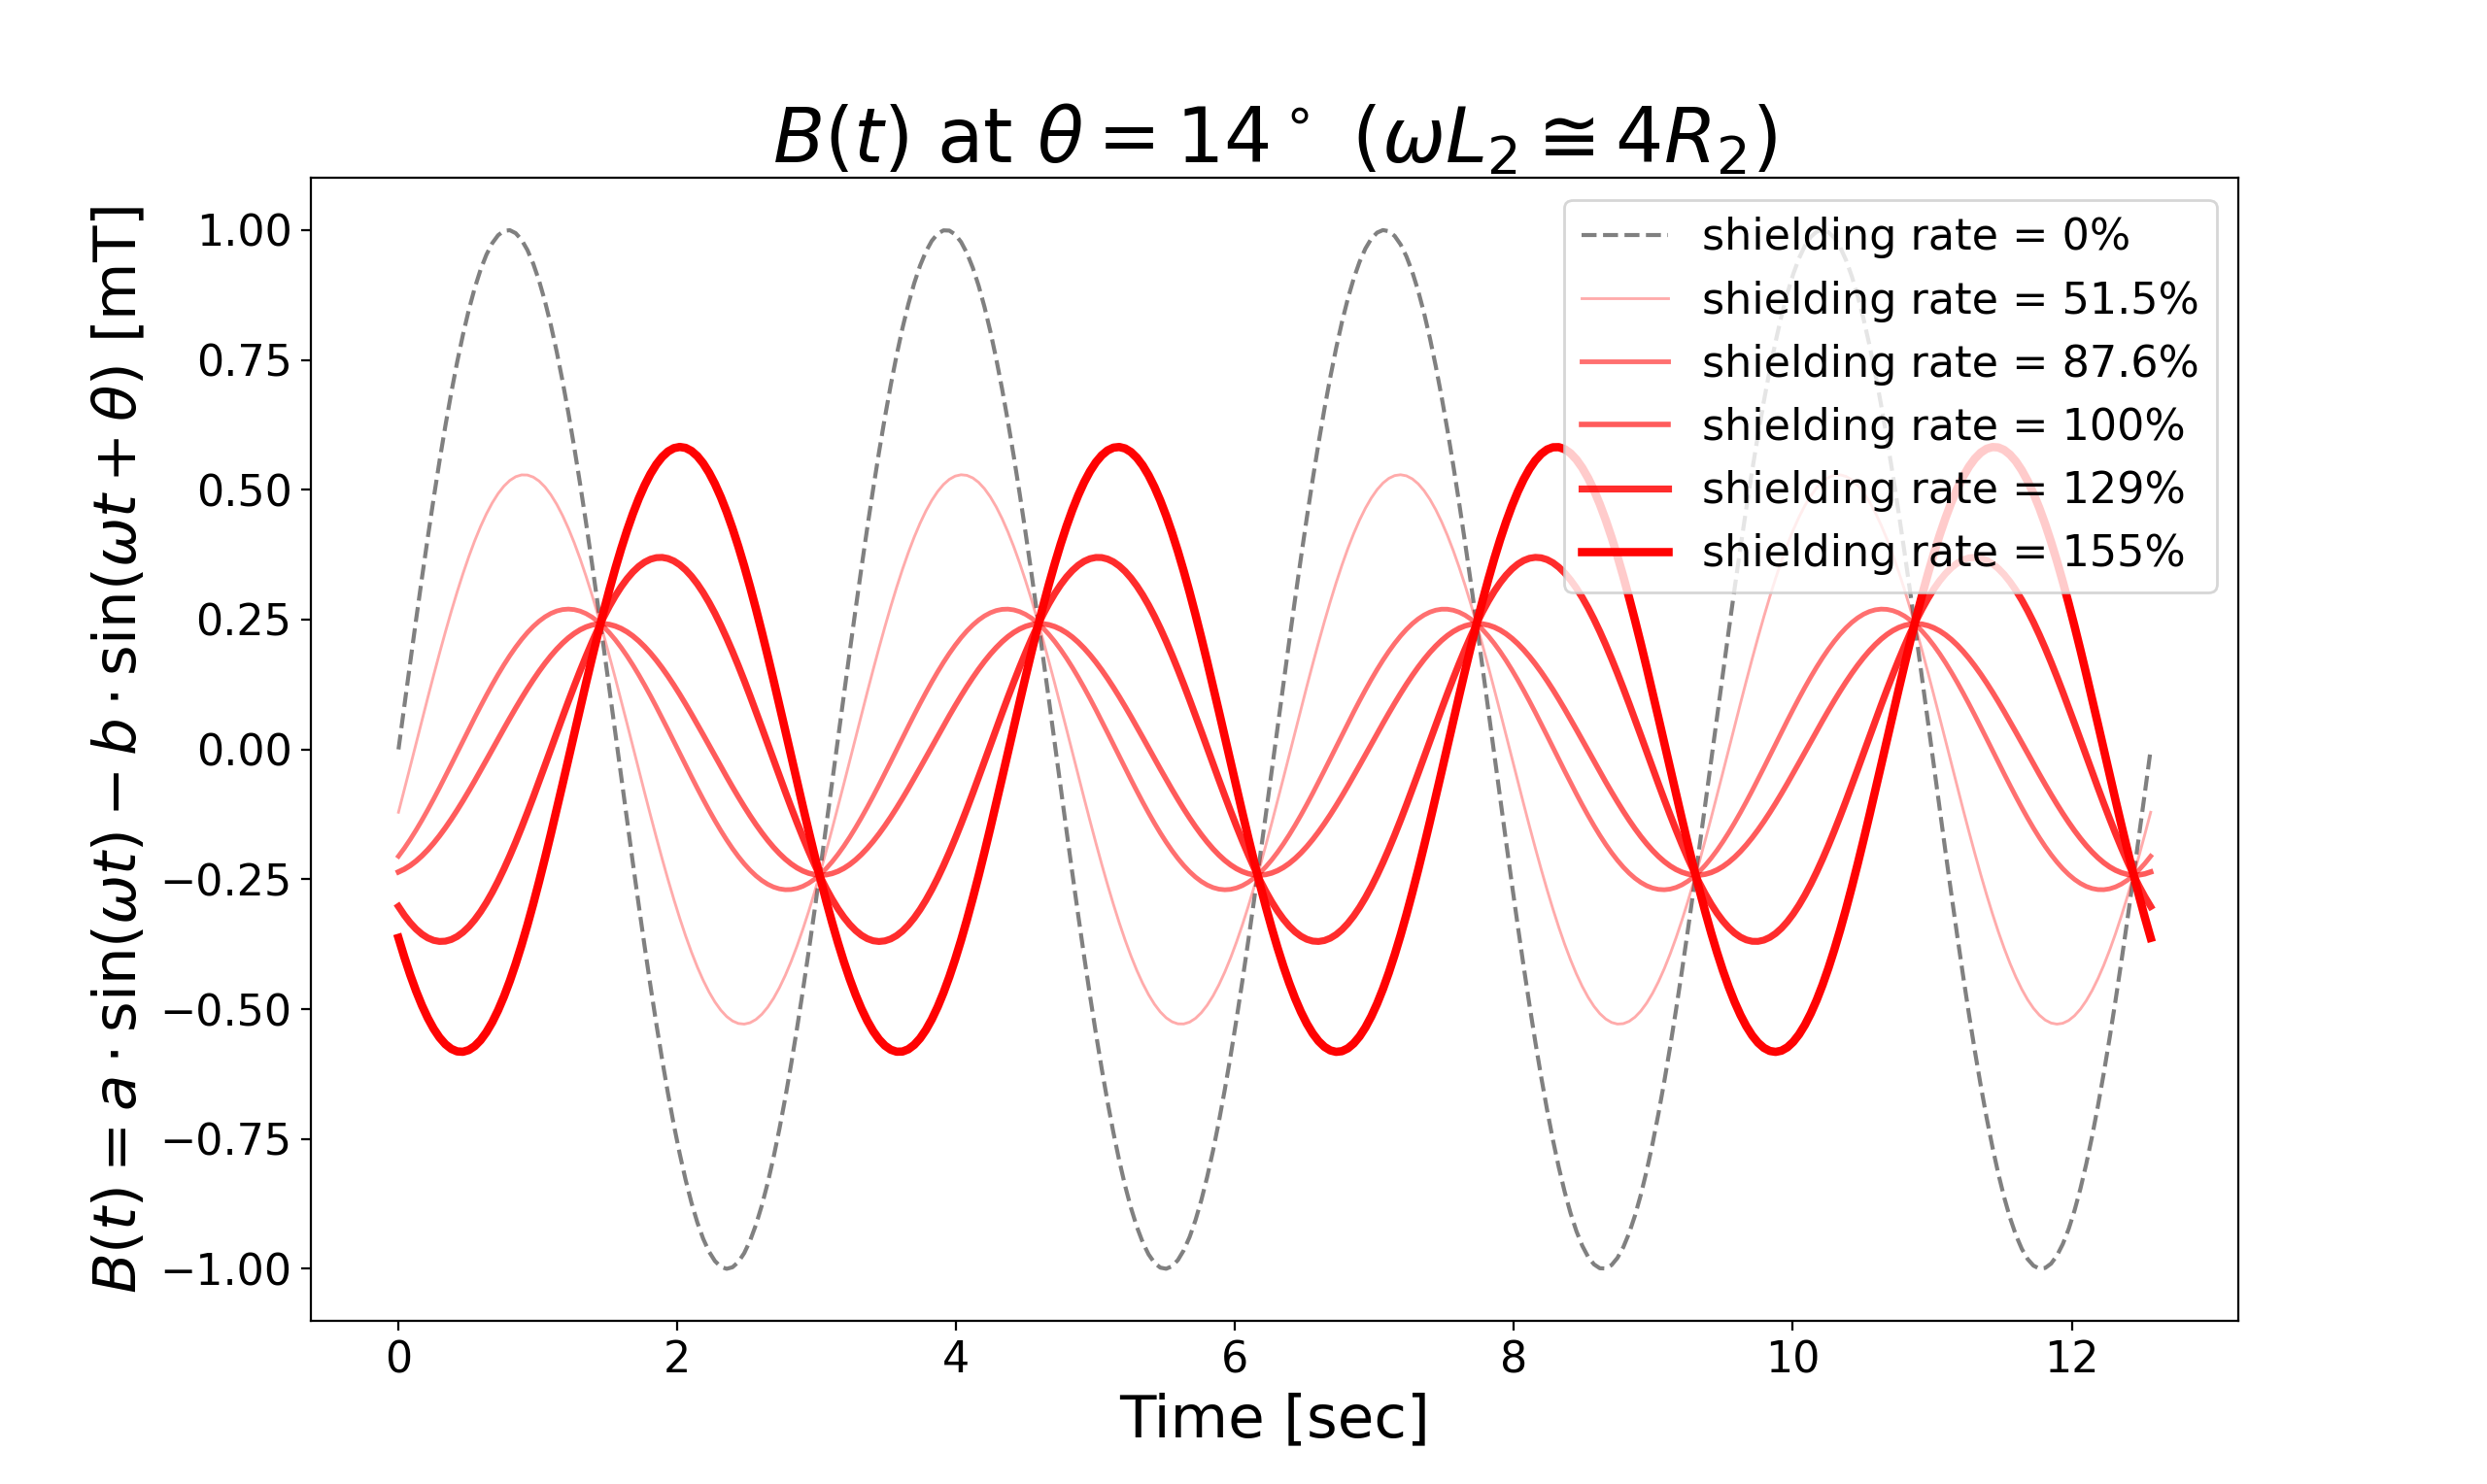
\includegraphics[width=17cm, bb=9 9 900 490]{./section3Effectiveness/sinTestAt14deg.png}
  \caption{Simulated $B$ using equation (40) with $\theta = 14^\circ$ ($\omega L_2 \cong 4R_2$).}
  \label{fig:14theta}
\end{figure}
From the above plots, in the condition that the induced current $i_2$ is delayed by $\theta$,
even if the shielding rate matches 100\% residual magnetic field $B$ remains none zero.

To sum it up, in a relatively small coil model with over shielding happened, the shielding rate would be small compared to a relatively large scale model.
Expand the measured $B$ data to a $\omega L \gg R$ condition raises the transparent points shown in Fig. \ref{fig:shieldingAbilityMeasuredShieldingRates}.
From which, shielding rates inside the coil around 100\% can be expected.
This expectation is close to the result of simulation, shown in the same graph by a transparent line.
It indicates that in a full scale model, a shielding rate at least 95\% is achievable,
which is suitable working as a magnetic field shielding system.


\subsubsection{Conclusion}
In this section, we have measured the shielding rates along the z axis on a scaled down model.
Although the measured shielding rate shows a peak of about 78\%,
in full scale models it can be epected to be over 95\%.
95\% shielding rate means the field inside the internal coil may be down to 50 mT when the external field is 1 T,
which is small enough for normal electrical equipments to work.
Needless to say, if more shielding is needed,
this system is free to be combined with any general magnetic field shielding system, such as the ones using normal ferromagnets.


\newpage
\subsection{Effect of Ferromagnets}
To avoid the weaking of the field near the shielding system,
we have proposed that inserting ferromagnets on the top of the superconductor coil,
expecting strong magnetization to reinceforce the field.
In this section, we have conducted a series of experiments to confirm the effect of ferromagnet.
As before, the purpose, the theory, the method and the result is shown in the following sections.

\subsubsection{Purpose}
The purpose of this experiment is to proof that ferromagnets do increase the field near the edge of the superconductor coil.

\subsubsection{Theory}
In section 2.3 we have already introduced the physical foundation of the ferromagnetism,
which is,
strong magnetization $M$ in a ferromagnet would be induced even though the imposed field is weak.
The equation
\begin{equation}
  B = M + \mu_0 H
\end{equation}
must hold.
Although the direction of $M$ is not always strictly identical with $B$ and $H$,
the direction is almost the same.
In the following paragraphs, further discussion about the $B$ and $M$ field is denoted,
approaching from the vector potential.

Consider an Electromagnetic Induction type magnetic cloak model, with curve ferromagnets placed in the upper and lower edge,
as shown in Fig. \ref{fig:EIMC_modelWithFM}.
Note that only the internal coil and ferromagnet are plotted,
the external coil are ommited here.
\begin{figure}[H]
  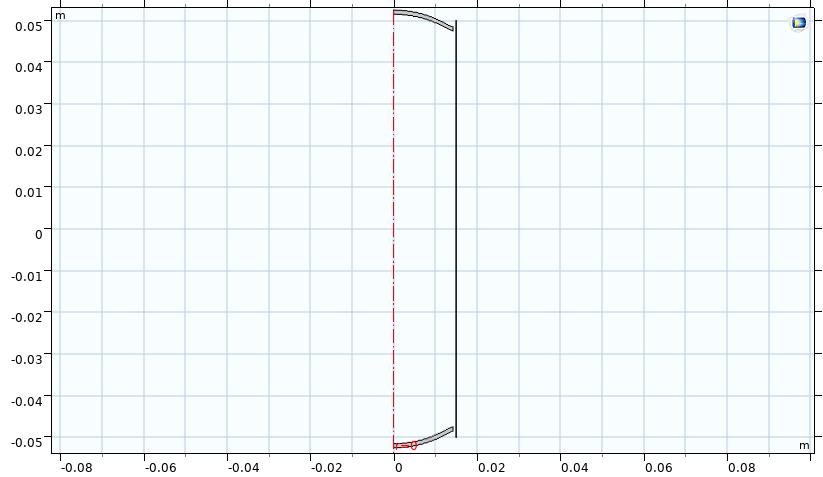
\includegraphics[width=17cm, bb=9 9 900 550]{./section3Effectiveness/plannedFM2Structure.png}
  \caption{The axisymmetric model used in our simulation. Note that only the inner coil is plotted here.}
  \label{fig:EIMC_modelWithFM}
\end{figure}
A cylindrical coordinates $(\rho, \phi, z)$ is used in this model,
in which the vector potential $\mathbf{A}_p(\rho, 0, z)$ at point $p(\rho, 0, z)$ is the combination of
the potential generated by the coil $\mathbf{A}_{coil}$,
the potential generated by the outer surface of the upper magnet $\mathbf{A}_{magUpperSurface}$,
and the potential generated by the inner surface of the upper magnet $\mathbf{A}_{magLowerSurface}$,
\begin{eqnarray}
  \mathbf{A}_p(\rho, 0, z) &=& \mathbf{A}_{coil} + \mathbf{A}_{magUpperSurface} + \mathbf{A}_{magLowerSurface}\\\nonumber
  &=& \sum_{i=1}^{N}\frac{\mu_0I_1}{\pi k_c}\sqrt{\frac{\rho'_c}{\rho}}\left((1-\frac{1}{2}k_c^2)K(k_c) - E(k_c)\right)\\\nonumber
  &+& \int_{Z_{LO}}^{Z_{UO}}dz'_{mO}\cdot\frac{\mu_0k_{\phi'}}{\pi k_{mO}}\sqrt{\frac{\rho'_{mO}(z'_{mO})}{\rho}}\left((1-\frac{1}{2}k_{mO}^2)K(k_{mO}) - E(k_{mO})\right)\\\nonumber
  &+& \int_{Z_{LI}}^{Z_{UI}}dz'_{mI}\cdot\frac{\mu_0k_{\phi'}}{\pi k_{mI}}\sqrt{\frac{\rho'_{mI}(z'_{mI})}{\rho}}\left((1-\frac{1}{2}k_{mI}^2)K(k_{mI}) - E(k_{mI})\right)\mathbf{e}_{\phi}\\\nonumber
  &,& K(k) = \mathrm{TheFirstKindCompleteEllipticIntegralWithModulus} k\\\nonumber
  &,& E(k) = \mathrm{TheSecondKindCompleteEllipticIntegralWithModulus} k\\\nonumber
  &,& k_c = \sqrt{\frac{4\rho\rho'_c}{(\rho+\rho'_c)^2+(z-z'_{ci})^2}}\\\nonumber
  &,& k_{\phi'} = (\mathbf{M}\times\mathbf{n})_{\phi'}\\\nonumber
  &,& k_{mO} = \sqrt{\frac{4\rho\rho'_c}{(\rho+\rho'_c)^2+(z-z'_{mO})^2}}\\\nonumber
  &,& k_{mI} = \sqrt{\frac{4\rho\rho'_c}{(\rho+\rho'_c)^2+(z-z'_{mI})^2}}\nonumber
\end{eqnarray}
where $\rho'_c$ represents the coil's radius,
$z'_{ci}$ represents the z position of the $i$th turn,
$z'_{mO}$ represents the z position of the outer magnet surface varying from $Z_{LO}$ to $Z_{UO}$,
$z'_{mI}$ represents the z position of the inner magnet surface varying from $Z_{LI}$ to $Z_{UI}$,
$\rho'_{mO}(z)$ represents the radius distribution of the outer magnet surface which is a function of $z'_{mO}$,
$\rho'_{mI}(z)$ represents the radius distribution of the inner magnet surface which is a function of $z'_{mI}$.
Mark that in equation (43) only the magnetization $\mathbf{M}$ and the induced current $I_1$ are variables,
once they are determined the vector potential can be solved directly.
However, even though we can solve the induced current term by Bio-Savart's law,
the magnetization terms are hard to solve.
Therefore, we have used the finite element method to solve it numerically.


\subsubsection{Method}
To measure the effect of ferromagnets, we have conducted a series of simulation and experiments.
Two internal coil models have been evaluated,
one with ferromagnets placed on the top and bottom edge of the superconductor coil,
another only the superconductor coil.
The superconductor coils here are not simple solenoid windings as the ones used in the previous sections,
but are windings with more turns near the edge and less turns at the central,
which we name it the "distributed coil".
The parameters of the equipments are shown in Tab. \ref{tab:distributedCoil},
and a photograph of the actual distributed coil windings is shown in Fig. \ref{fig:photoDistributedCoil}.
\begin{figure}[H]
  \includegraphics[width=9.5cm, bb=9 9 900 1500]{./section3Effectiveness/distributedCoil.png}
  \caption{The distributed coil under test.}
  \label{fig:photoDistributedCoil}
\end{figure}
\begin{table}[H]
  \centering
  \caption{Specification of the experiment.}
  \label{tab:distributedCoil}
  \begin{tabular}{cccc}\hline\hline
    Parameter & Distributed Coil with Ferromagnet & Distributed Coil without Ferromagnet & External Coil \\\hline
    Diameter [cm] & 3.0 & 3.0 & 14\\\hline
    Length [cm] & 10 & 10 & 20 \\\hline
    Turns & 50 & 50 & 40 \\\hline
    Critical Current $I_C$ [A] & 120 & 120 & Copper \\\hline
    Width of Superconductor Tape & 4 & 4 & -\\\hline\hline
  \end{tabular}
\end{table}

For the simulation,
we have used the finite element method provided by commercial software Comsol Multiphysics Inc. to solve the vector potential $A$ around the model,
and latter derived the magnetic field distribution from the potential field.
The external field we used is a model of MRI coils, of which the detail would be describe in chapter 5.
Since it is almost uniform within the internal space, it can be considered uniform field here.

For the experiment,
we have made the two coils as denoted above, with one of which covered by a $0.6$ mm ferit sheet.
Due to the central part of the windings being sparse,
we have also placed a layer of ferit sheet on the inner wall of the FM model to see if the it can perform any shielding effect to increase the shielding effect.
The procedure of the experiment is the same as the one conducted in the previous section,
with AC imposed fields and the axis field measured.


\subsubsection{Result and Discussion}
The simulated magnetic field distribution of the model include ferromagnet is shown in Fig. \ref{fig:simulation_withFM},
and that of the model without ferromagnet is show in Fig. \ref{fig:simulation_withoutFM}.
Note that only the area near the top edge is plotted.
\begin{figure}[H]
  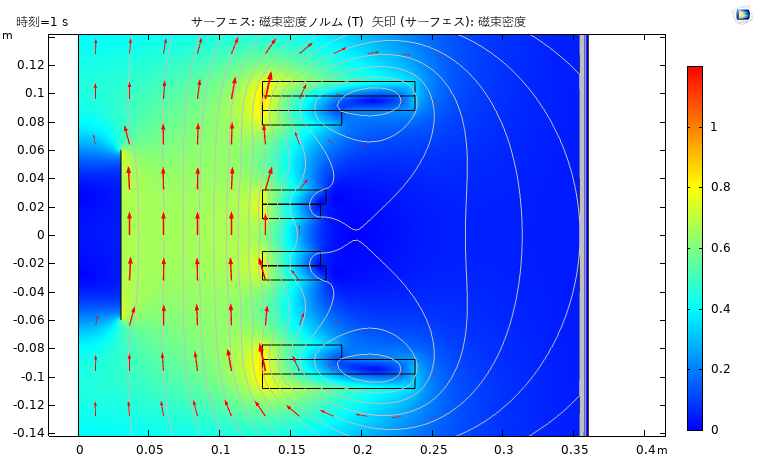
\includegraphics[width=17cm, bb=9 9 900 530]{./section3Effectiveness/BnormDistributionInMRICoilWithoutFM.png}
  \caption{Simulated magnetic field without ferromagnet.}
  \label{fig:simulation_withoutFM}
\end{figure}
\begin{figure}[H]
  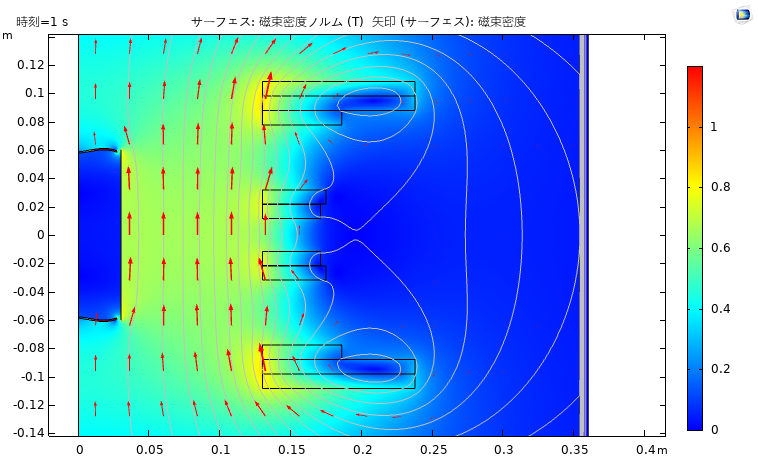
\includegraphics[width=17cm, bb=9 9 900 500]{./section3Effectiveness/BnormDistributionInMRICoilWithFM.png}
  \caption{Simulated magnetic field with ferromagnet.}
  \label{fig:simulation_withFM}
\end{figure}
Comparing the two results,
we can see that the model with ferromagnet actually has reinceforced the outer field near the coil,
and slightly increased the shielding effect on the inner side.
This calculation have confirmed that the inserting ferromagnets on the edge is effective to improve the cloaking ability.

To double check the effect,
an experiment measured the shielding rate along the z axis has been conducted.
The result of measured $B$ field is shown in Fig. \ref{fig:expFMMeasuredBs},
and that of measured shielding rates is shown in Fig. \ref{fig:expFMMeasuredShieldingRates}.
\begin{figure}[H]
  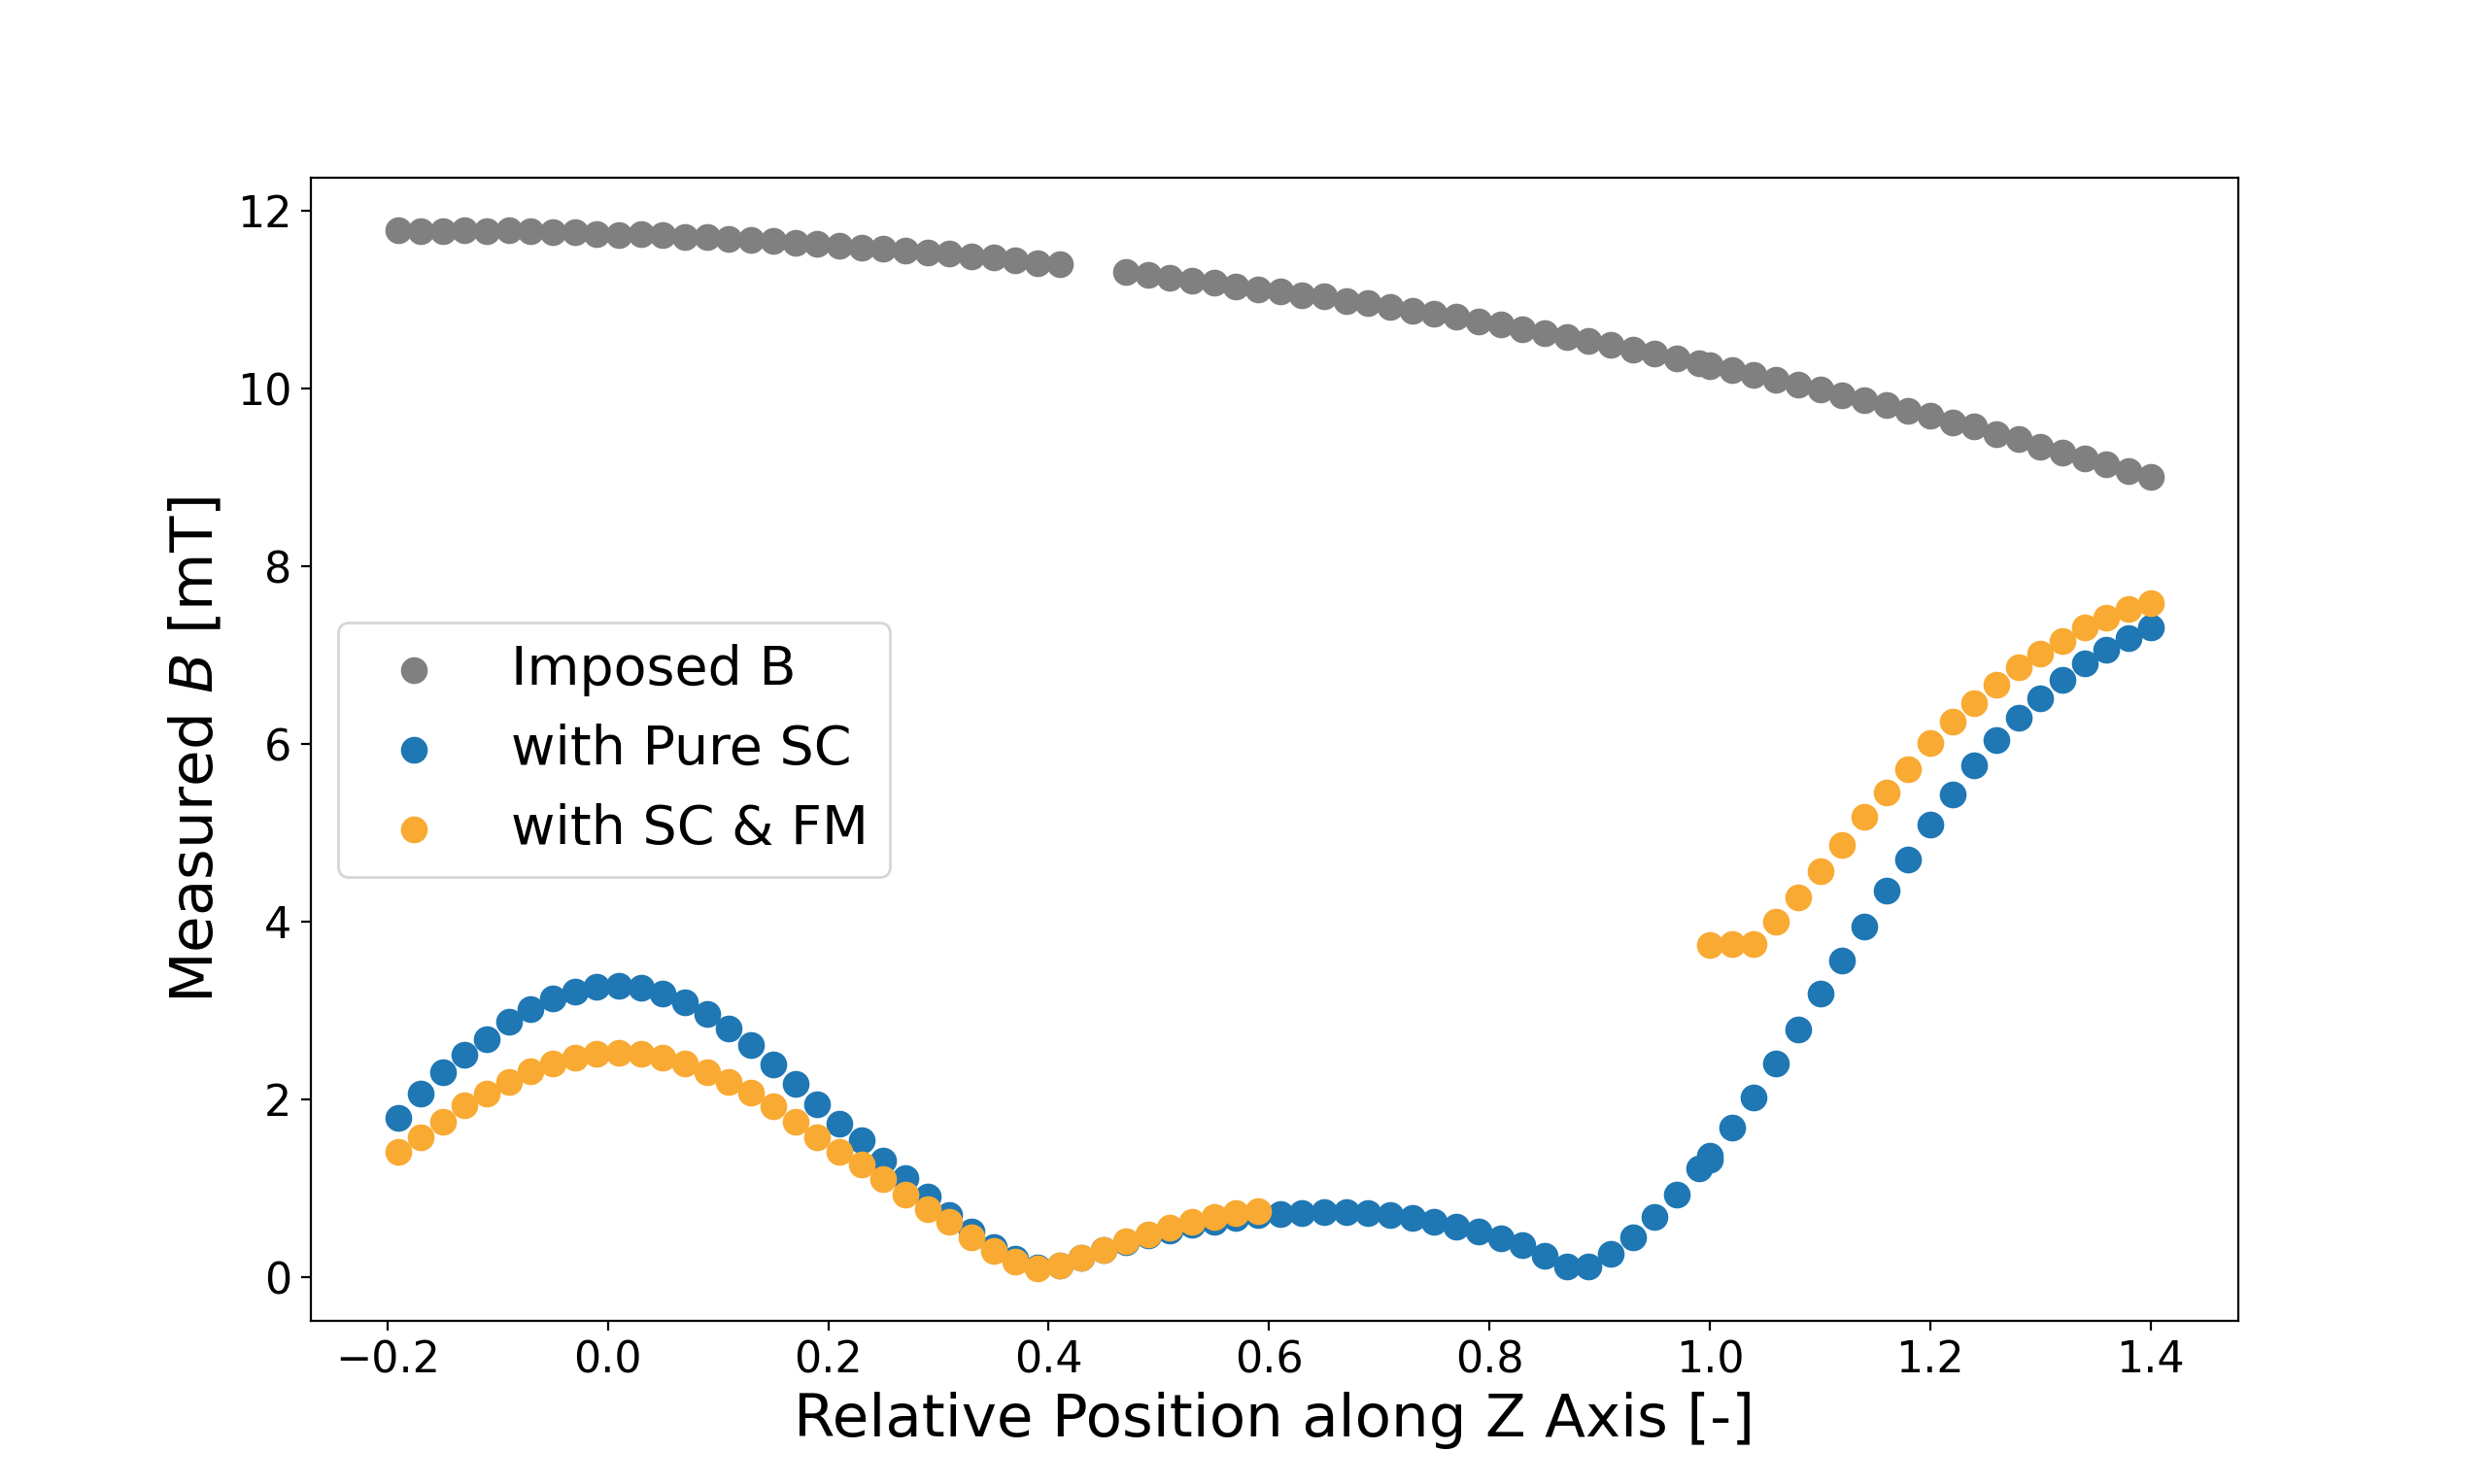
\includegraphics[width=18cm, bb=9 9 900 550]{./section3Effectiveness/comparedB.png}
  \caption{Measured $B$ field along the axis.}
  \label{fig:expFMMeasuredBs}
\end{figure}
\begin{figure}[H]
  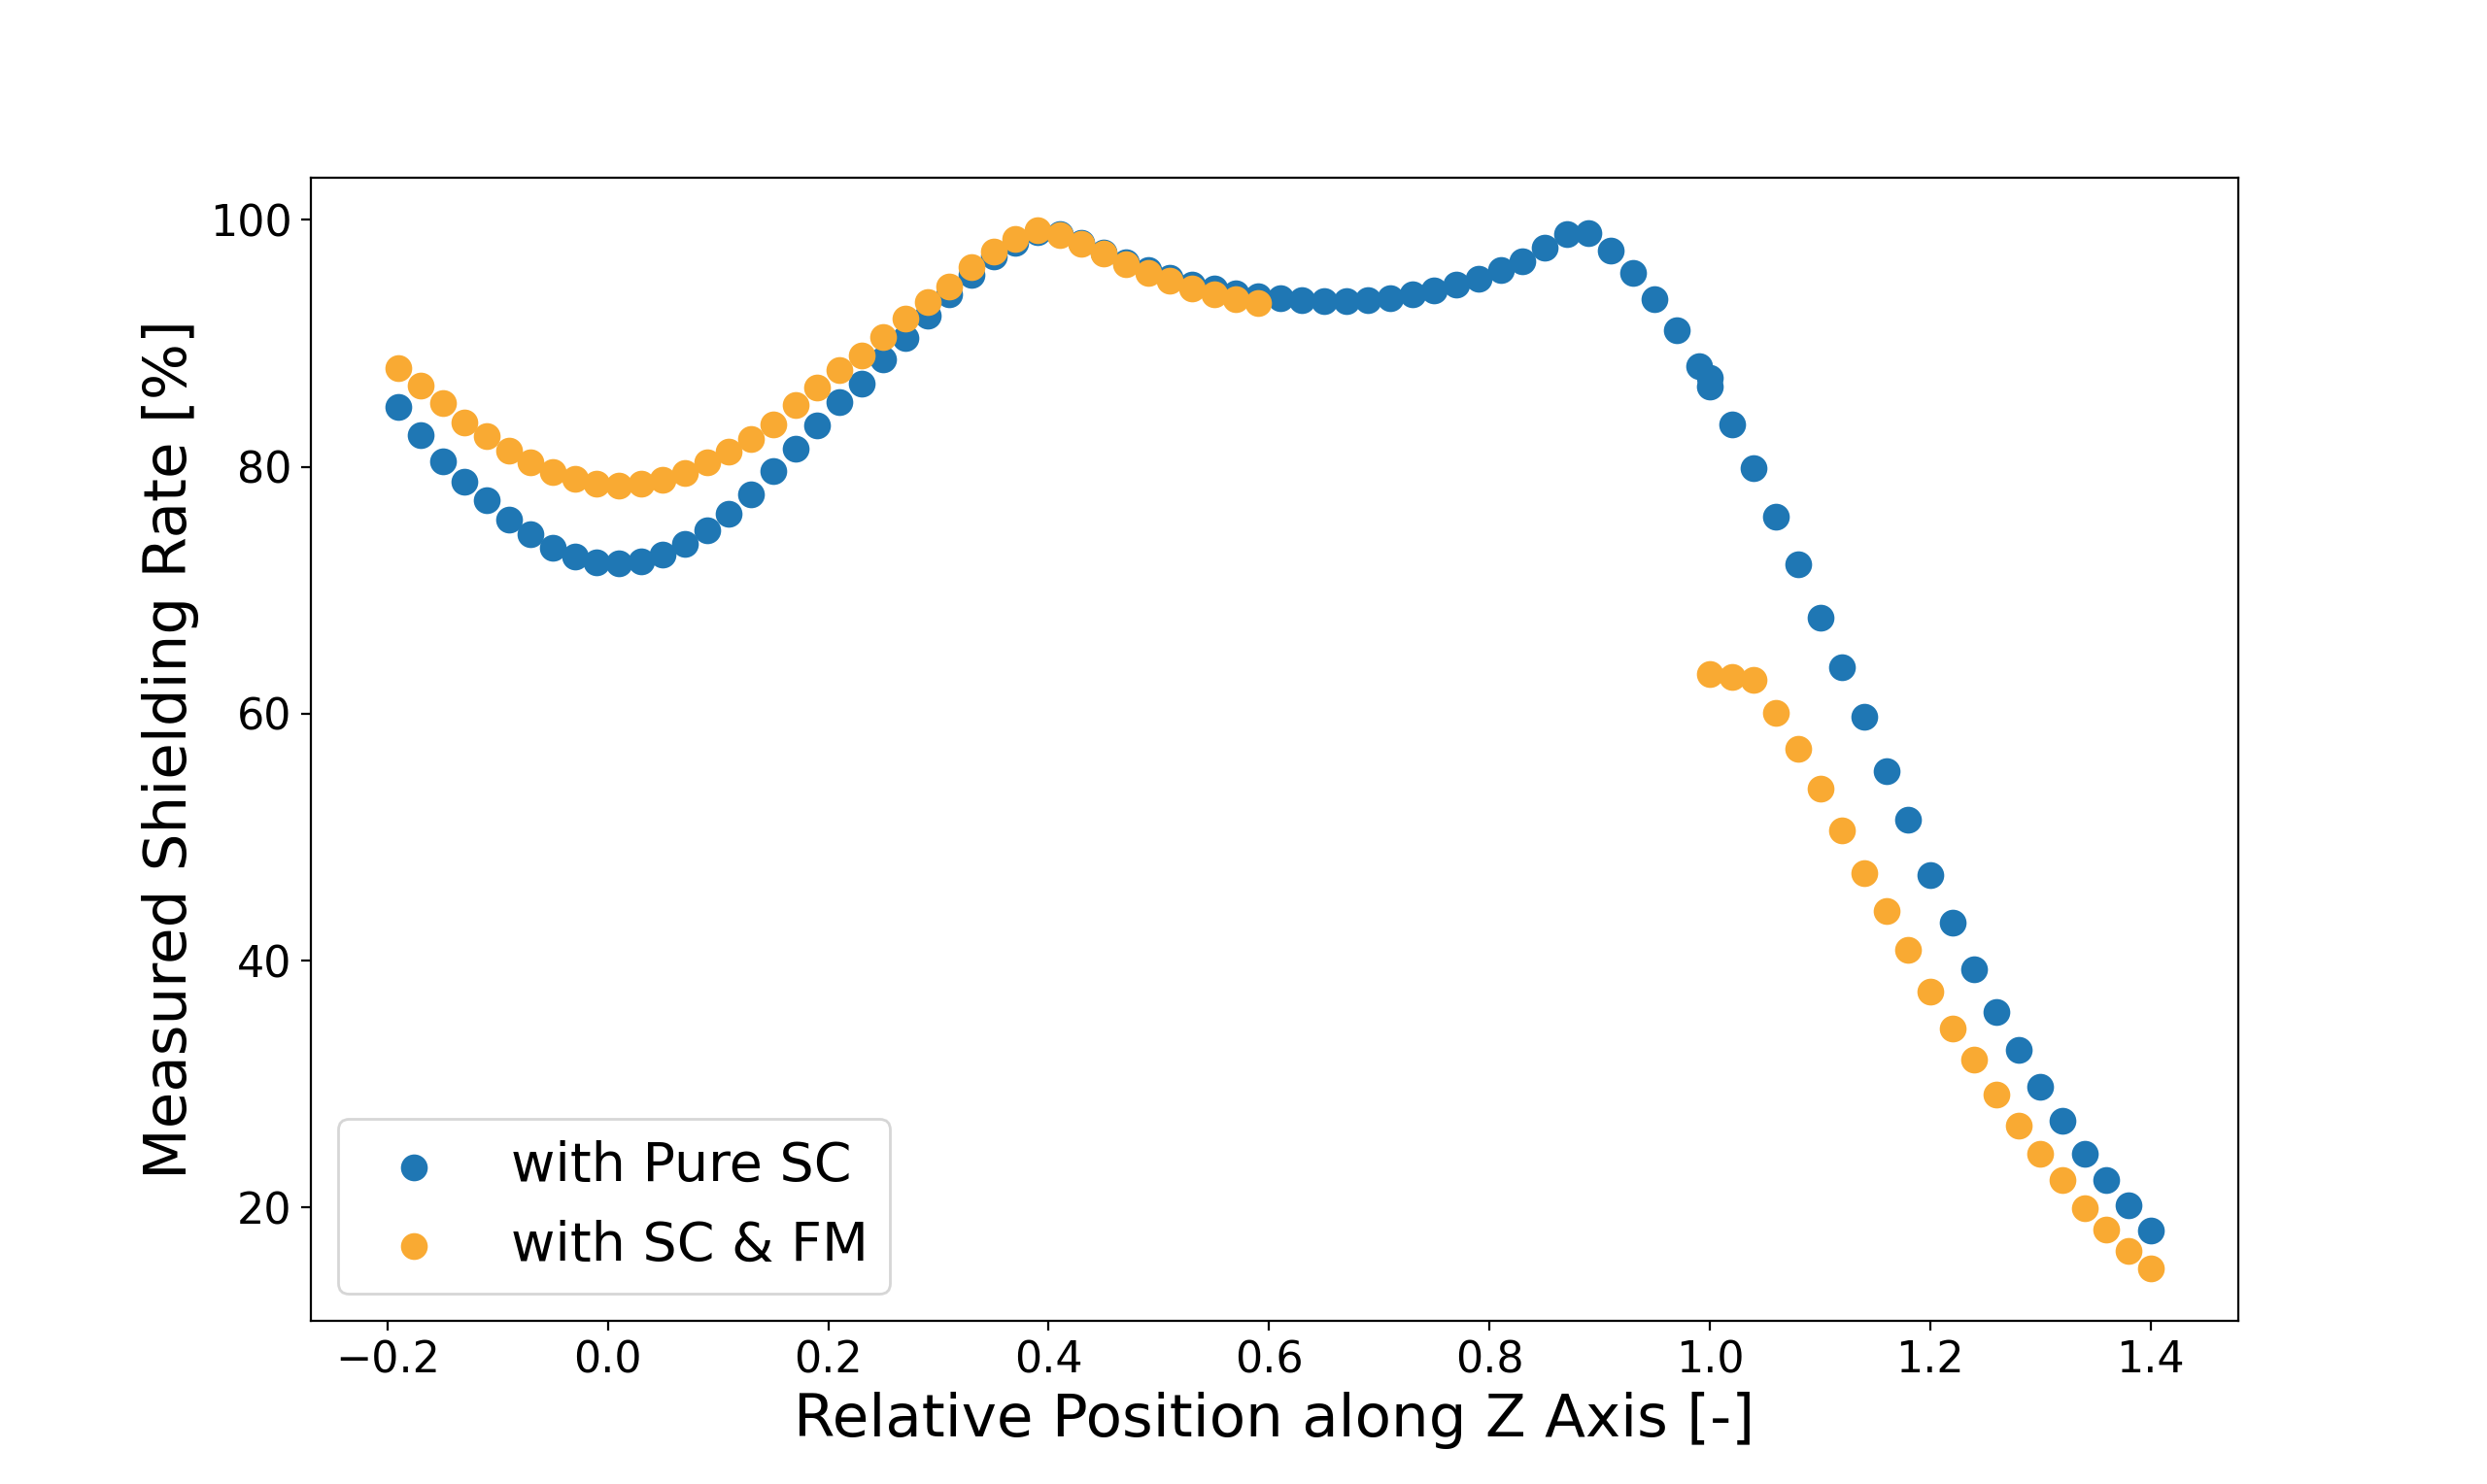
\includegraphics[width=18cm, bb=9 9 900 550]{./section3Effectiveness/comparedShieldingRate.png}
  \caption{Measured shielding rate along the axis.}
  \label{fig:expFMMeasuredShieldingRates}
\end{figure}
From the two figures,
we can seen that with the ferromagnet, the outer field is compensated, and the inner field is further shielded.
This result agrees with the simulated one,
both indicating that placing ferromagnets on the surface of the coil is effective to increase the cloaking ability.


\subsubsection{Conclusion}
In this section, the result of simulation and experiments has shown that placing ferromagnet at the top and bottom surface of the internal coil is able to increase the cloaking ability,
which is to reinforces the outer magnetic field and eliminating the inner magnetic field.
This indicates that a magnetic cloak able to operate in several T field is possible through our proposal using high temperature superconductor tapes and ferromagnets.
To step further,
the optimized construction of the Electromagnetic Induction Type Magnetic Cloak is shown in the next chapter.


\newpage
\section{Optimal Construction of the Electromagnetic-Induction Type Magnetic Cloak}
% section 4 Optimized Construction
In the previous chapters, we have shown that all the proposed Electromagnetic Induction Type Magnetic Cloak is effective as a shielding system under high fields up to several Tesla.
In this chapter, we show the optimal construction of our proposal, aim to maximize the shielding rate inside and the reinforcement of magnetic field outside.

Since the proposed cloak consists of superconductor windings and ferromagnets,
and both parts influence the magnetic field,
we have investigated them respectively.
For the fact that the superconducting windings generates magnetic field covering much more wider range than the ferromagnetic,
it is consider proper to first optimize the parameters of the windings then that of the magnets.
Just as optimizing the two variables function $f(x, y) = 100x + y$,
it is obvious that $x$ is more significant to the value of $f$ and thus should be first determined.
In the following sections, we first deliver the result of the optimal construction of the superconducting coil,
and then the result of the optimal position of ferromagnets.


\newpage
\subsection{Optimal Construction of the High Temperature Superconductor Windings}
As a EIMC, the minimum request is for the windings to form a closed loop.
Obviously, there are many methods and approach for this goal.
The simplest way can be conventional solenoid coils, with the top and bottom turn shorted.
Theese solenoid coils are easy to manufact when the scale is small,
with the electrical resistance being limited.
Thus scaled down models used in our experiments described in the previous chapters are all solenoid like windings.

Another possible way is like the MRI coil windings, which consist of layered coils stack on each other.
The stacked coils are all electrically connected, satisfying the closed loop condition.
Compared to solenoid windings, the stacked coils can each be manufactored and transported respectively,
making it suitable for large scale models.
On the other hand, since in this way the connected parts amount would become comparatively more,
causing the resistance to increase and the time constant to drop,
the stacked coil is not ideal in a small scale model.

Anyway, the two coil patterns both give the same magnetic field distribution if every turn is placed in the same position.
Therefore, due to the small scale of our experimental models,
we have used the solenoid winding in all the experiments.
For the numerical calculation, we have used 2D axisymmetric model in which the winding method is not considered.

In this section, we have attempted to figure out the best construction of the windings,
by a series of optimization and experiments.
As the same as before, the purpose, the theory, the methods and the result are noted.


\subsubsection{Purpose}
If the position of the turns changed, the magnetic field nearby would changed.
Therefore, the optimal construction of the coil exists such that
the best cloak property minimizing the penetrating field and maximizing the field near the top and bottom surface is achieved.
The purpose of this section is to discover this optimized solution of coil construction.


\subsubsection{Theory}
The optimization problem can be interpreted as, find the optimal position of every turn of the internal coil which minimize the inner $B$ field and maximize the outer $B$ field.
The mathmetical description can be written as below.
\begin{eqnarray}
  min\cdot loss(\mathbf{x}) = mean\left(|\mathbf{B}_{in}(\mathbf{x})|\right) - mean\left(|\mathbf{B}_{out}(\mathbf{x})|\right)
\end{eqnarray}
where $\mathbf{x}$ represents the positions of every specific turn constructing the internal coil,
$\mathbf{B}_{in}$ represents the $B$ field inside the internal coil,
$\mathbf{B}_{out}$ represents the $B$ field outside the internal coil,
and $loss$ represents the loss function (or the objective function) of the optimization problem.
Note that $\mathbf{B}$ and $loss$ are all functions of the coil position $\mathbf{x}$,
which simply indicates that changing on the position causes changing on every other functions.
The evaluation area which the average $\mathbf{B}_{in}$ and $\mathbf{B}_{out}$ are calculated remains controversial.
For $\mathbf{B}_{in}$ we have chosen the whole internal space,
while for $\mathbf{B}_{out}$ an area of 2 times the coil diameter $\times$ 1 times the coil height above the top surface has been chosen.
Any evaluation area wider than this would make little different on the solution,
since the magnetic field decays in $1/r^2$ from the source current.
The specification of the coil are shown in Tab.\ref{tab:optimizationOfCoilSpecification}
and the schematic drawing of the evaluation region is shown in Fig. \ref{fig:evaluationRegion}.
\begin{table}[H]
  \centering
  \caption{Specification of the coils used in simulation.}
  \label{tab:optimizationOfCoilSpecification}
  \begin{tabular}{ccc}\hline\hline
    Parameter & Internal Superconductor Coil & External Coil \\\hline
    Diameter [cm] & 3.0 & 14\\\hline
    Length [cm] & 12 & 20 \\\hline
    Turns & -(varying) & 40 \\\hline
    Width of Superconductor Tape & 4 & -\\\hline\hline
  \end{tabular}
\end{table}
\begin{figure}[H]
  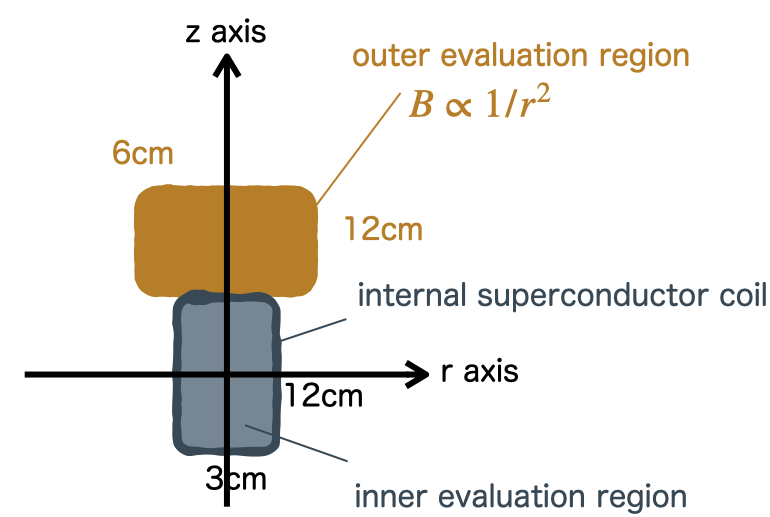
\includegraphics[width=18cm, bb=9 9 900 610]{./section4Optimal/evaluationRegion.png}
  \caption{Outer and inner field evaluation region.}
  \label{fig:evaluationRegion}
\end{figure}

This problem can be classified into the {\sl discrete nonlinear} optimization problem,
since the loss function is nonlinear to the variable $\mathbf{x}$ and
the turn position is limited to the fix tape width, which makes $\mathbf{x}$ to take discrete values.
Due to the solution space being discrete, we don't have many choices to solve it.
Among which includes the dynamic programming, the greedy method, the genetic algorithm and the modern machine learning methods like the reinceforcement learning, etc.
Here, to reach a comparatively general solution with limited calculation resource,
we have chosen the genetic algorithm which is able to explain the problem straight forward.
The detail is shown in the Method section.


\subsubsection{Method}
Within our calculation models, positions and fields are all calculated in 2D axisymmetric cylindrical coordinates $(r, z)$.
For instance, Fig. \ref{fig:coilDistributionSolenoid} shows a 2 layered solenoid windings,
with 30 turns per layer, 60 turns totally.
Note that since the length of the internal coil is 12 cm and the width of superconductor tape is 4 mm,
as shown in Tab. \ref{tab:optimizationOfCoilSpecification},
this is one of the simplest windings to fill up the whole length of the coil winding frame.
\begin{figure}[H]
  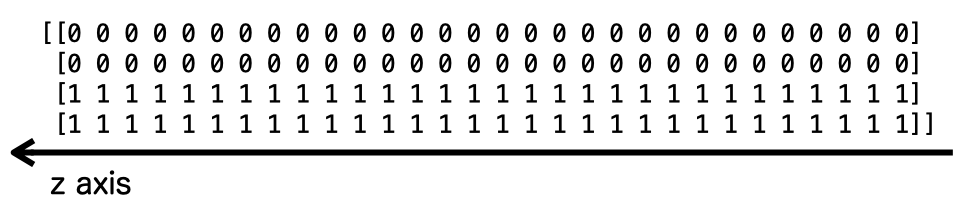
\includegraphics[width=18cm, bb=9 9 900 200]{./section4Optimal/solenoidCoilDistribution.png}
  \caption{Distribution of a solenoid windings.}
  \label{fig:coilDistributionSolenoid}
\end{figure}
For convenience, we named the axis parallel to the z axis "layer", the axis vertical to the z axis "stair".
In Fig. \ref{fig:coilDistributionSolenoid}, the windings have 2 layers and 30 stairs.

Next, we denote the method to produce next generation,
which we name "boom babies".
From any mother coil, we randomly choose 1 stairs to "grow" or "shrink".
The action "grow" means to stack one more turn on the specific stair,
while the action "shrink" means to remove one turn from the specific stair.
The maximum layer amount is set to be 4 for manufactoring reason,
and the minimum layer amount is zero.
Whether the selected stair should grow or shrink is also randomly chosen.
This action produces a "baby" coil from the "mother" coil.
Fig. \ref{fig:exampleDistribution} shows an example where the th stair is shrinked.
\begin{figure}[H]
  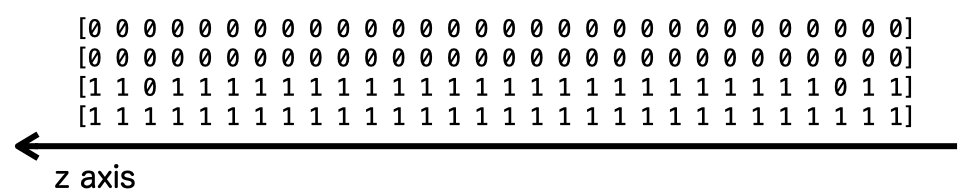
\includegraphics[width=18cm, bb=9 9 900 200]{./section4Optimal/exampleShrinkedCoil.png}
  \caption{Distribution of the coil shrinked from a 2 layered solenoid windigns.}
  \label{fig:exampleDistribution}
\end{figure}

The amount of individuals (coils) which can exist in each generation is set to 20.
For the begining of the calculation, we start with a normal 2 layered solenoid windings shown in Fig. \ref{fig:coilDistributionSolenoid}.
Since we only have 1 coil in the first generation, we boom 20 babies from this mother coil.
From the second generation, each coil booms 3 babies, results in all $20\times4 = 80$ (including mothor coils themself) coils.
From the 80 coils, we calculate their loss function and take the minimum 20 coils as survived individuals in the generation,
with the other 60 coils abandomed.
This is considered one step of the genetic algorithm.
When the average losses in the generation doesn't improve from the previous one,
we stop the calculation and take the least loss coil as the best solution.
The flow diagram of the program is shown in Fig. \ref{fig:flowOfGenetic}.
For the calculation of $B$ fields, the finite element method provided by commercial CAE software Comsol Multiphysics Inc. is used.
\begin{figure}[H]
  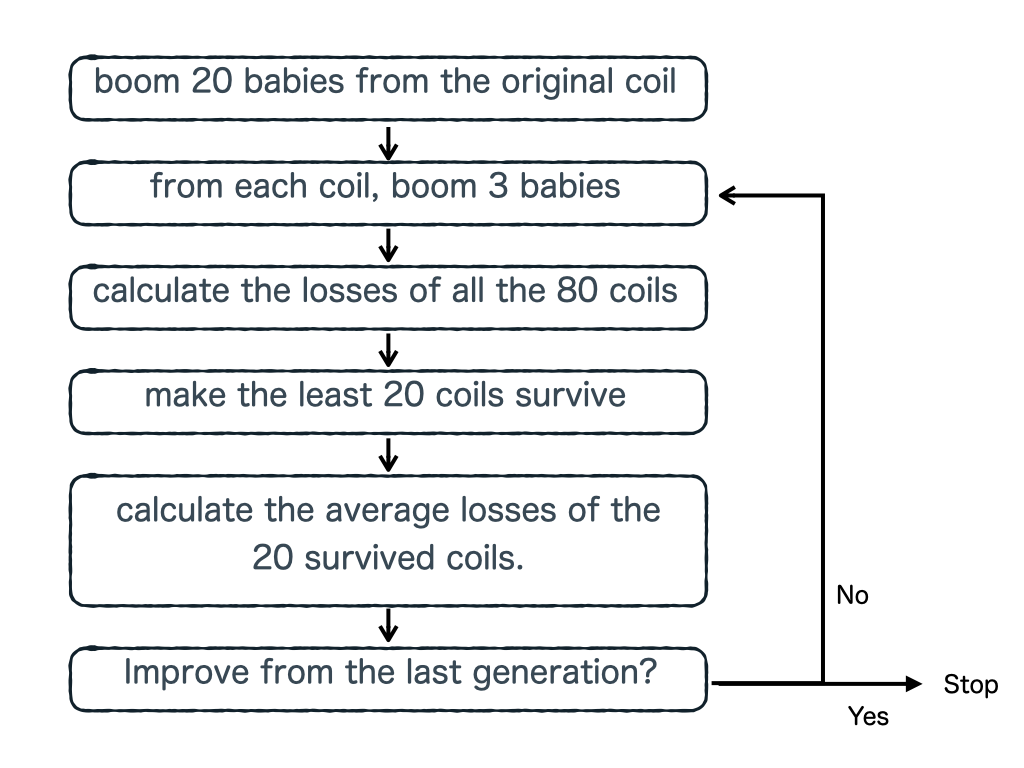
\includegraphics[width=18cm, bb=9 9 900 800]{./section4Optimal/geneticFlow.png}
  \caption{The flow of our genetic program.}
  \label{fig:flowOfGenetic}
\end{figure}

After the simulation, we have confirmed the result by an experiment.
Although the simluation has marked rectangular areas as evaluation region,
consider the accuracy of our equipment,
it is difficult ot measure the entire distribution in the evaluation resion.
Instead, we have taken the $B$ distribution along the z axis to represent the inner field,
and the $B$ distribution along the cross line on the top surface to represent the outer field.
The $B$ distribution on the both axises are measured and compared between the initial models and the optimized model.
Other details such as how the fields are measured are similar to the previous experiment,
and thus is ommited here.


\subsubsection{Result and Discussion}
The process of the optimization is shown in Fig. \ref{fig:optimizedCoilTrainingSteps},
and the initial solenoid coil and the ultimate optimized coil construction is shown in Fig. \ref{fig:optimizedCoilConstruction}.
\begin{figure}[H]
  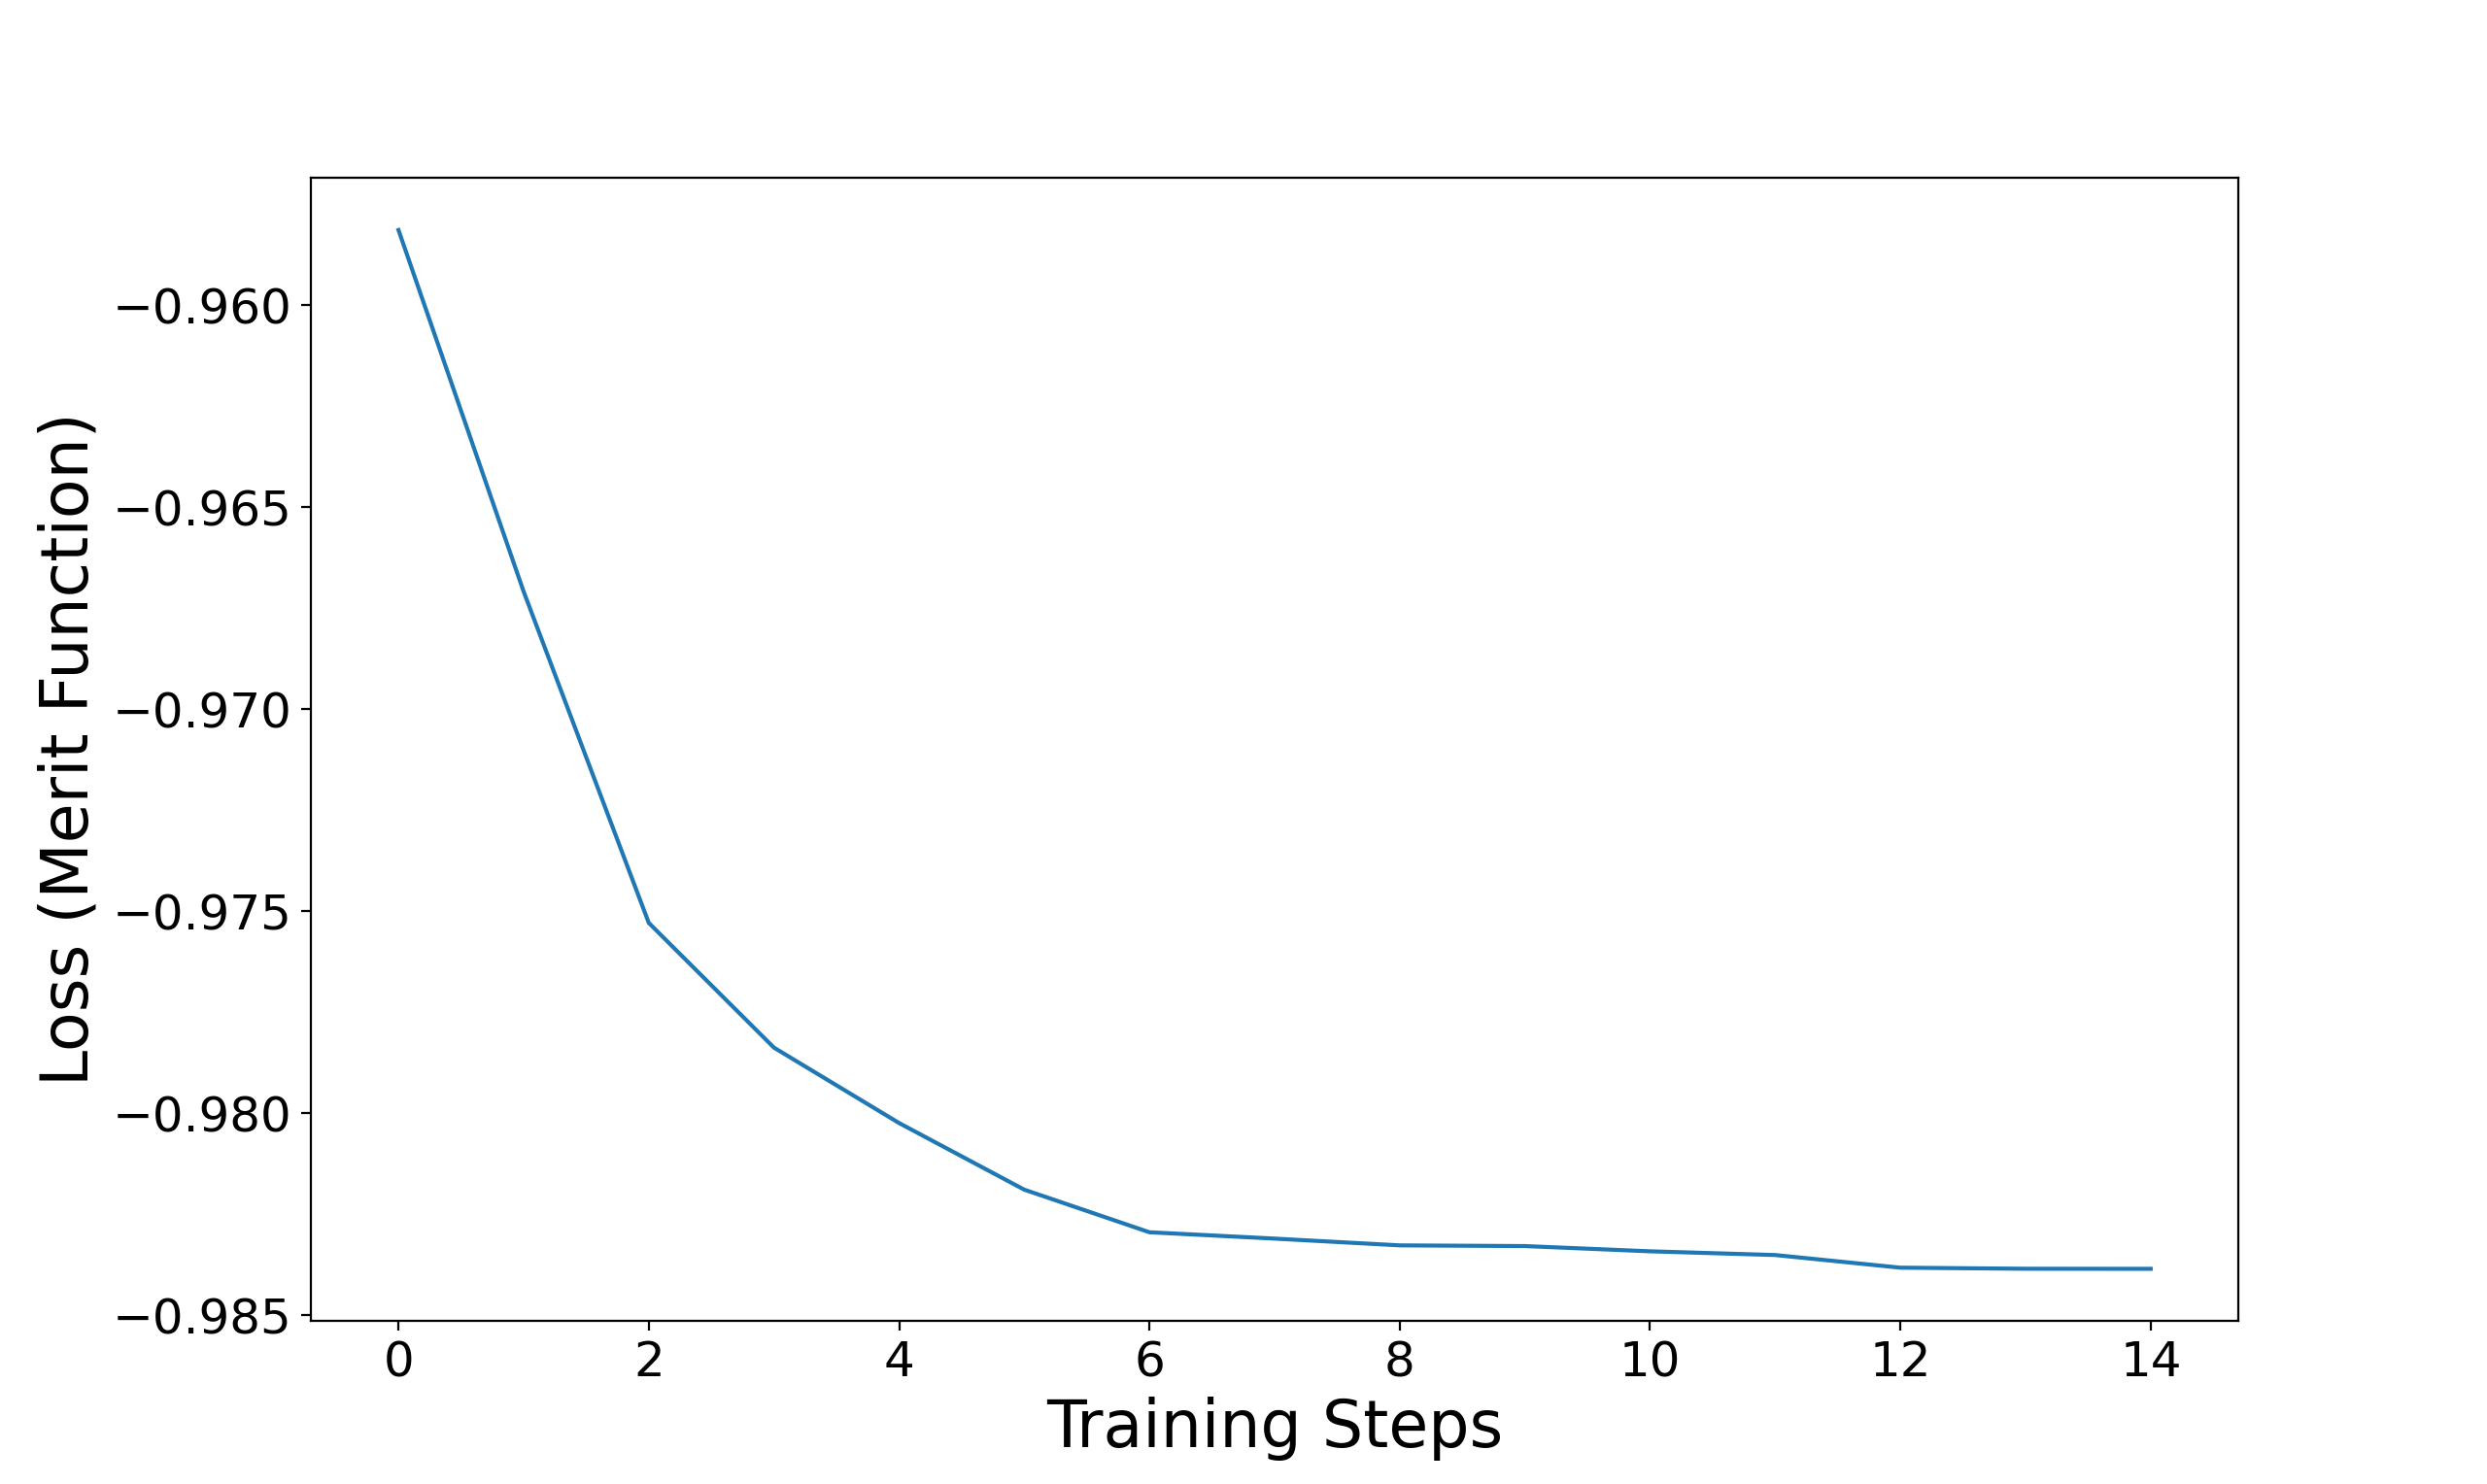
\includegraphics[width=18cm, bb=9 9 900 550]{./section4Optimal/averageLosses.png}
  \caption{Optimization process.}
  \label{fig:optimizedCoilTrainingSteps}
\end{figure}
\begin{figure}[H]
  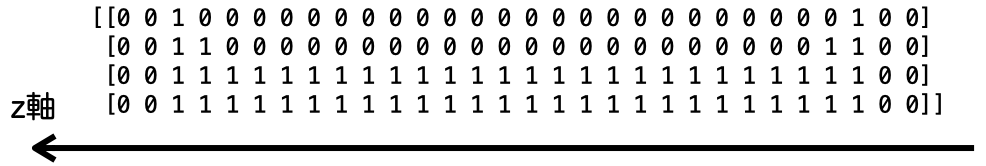
\includegraphics[width=18cm, bb=9 9 900 200]{./section4Optimal/optimizedCoilDistribution.png}
  \caption{Optimized coil distribution.}
  \label{fig:optimizedCoilConstruction}
\end{figure}
From Fig. \label{fig:optimizedCoilConstruction}, we can see that to achieve more cloaking ability,
more turns are needed near the edge and normal solenoid windings near the central part are just fine.
Also,

To confirm the calculation, we have manufacted the optimized coil and measured the shielding rates on the central axis and top cross line.
For comparison, the initial 2 layered solenoid coil are also manufacted and measured.
The experimental result along with the calculation are shown in Fig. \ref{fig:optimizedCoilExperimentResultCentral} and Fig. \ref{fig:optimizedCoilExperimentResultTopLine}.
\begin{figure}[H]
  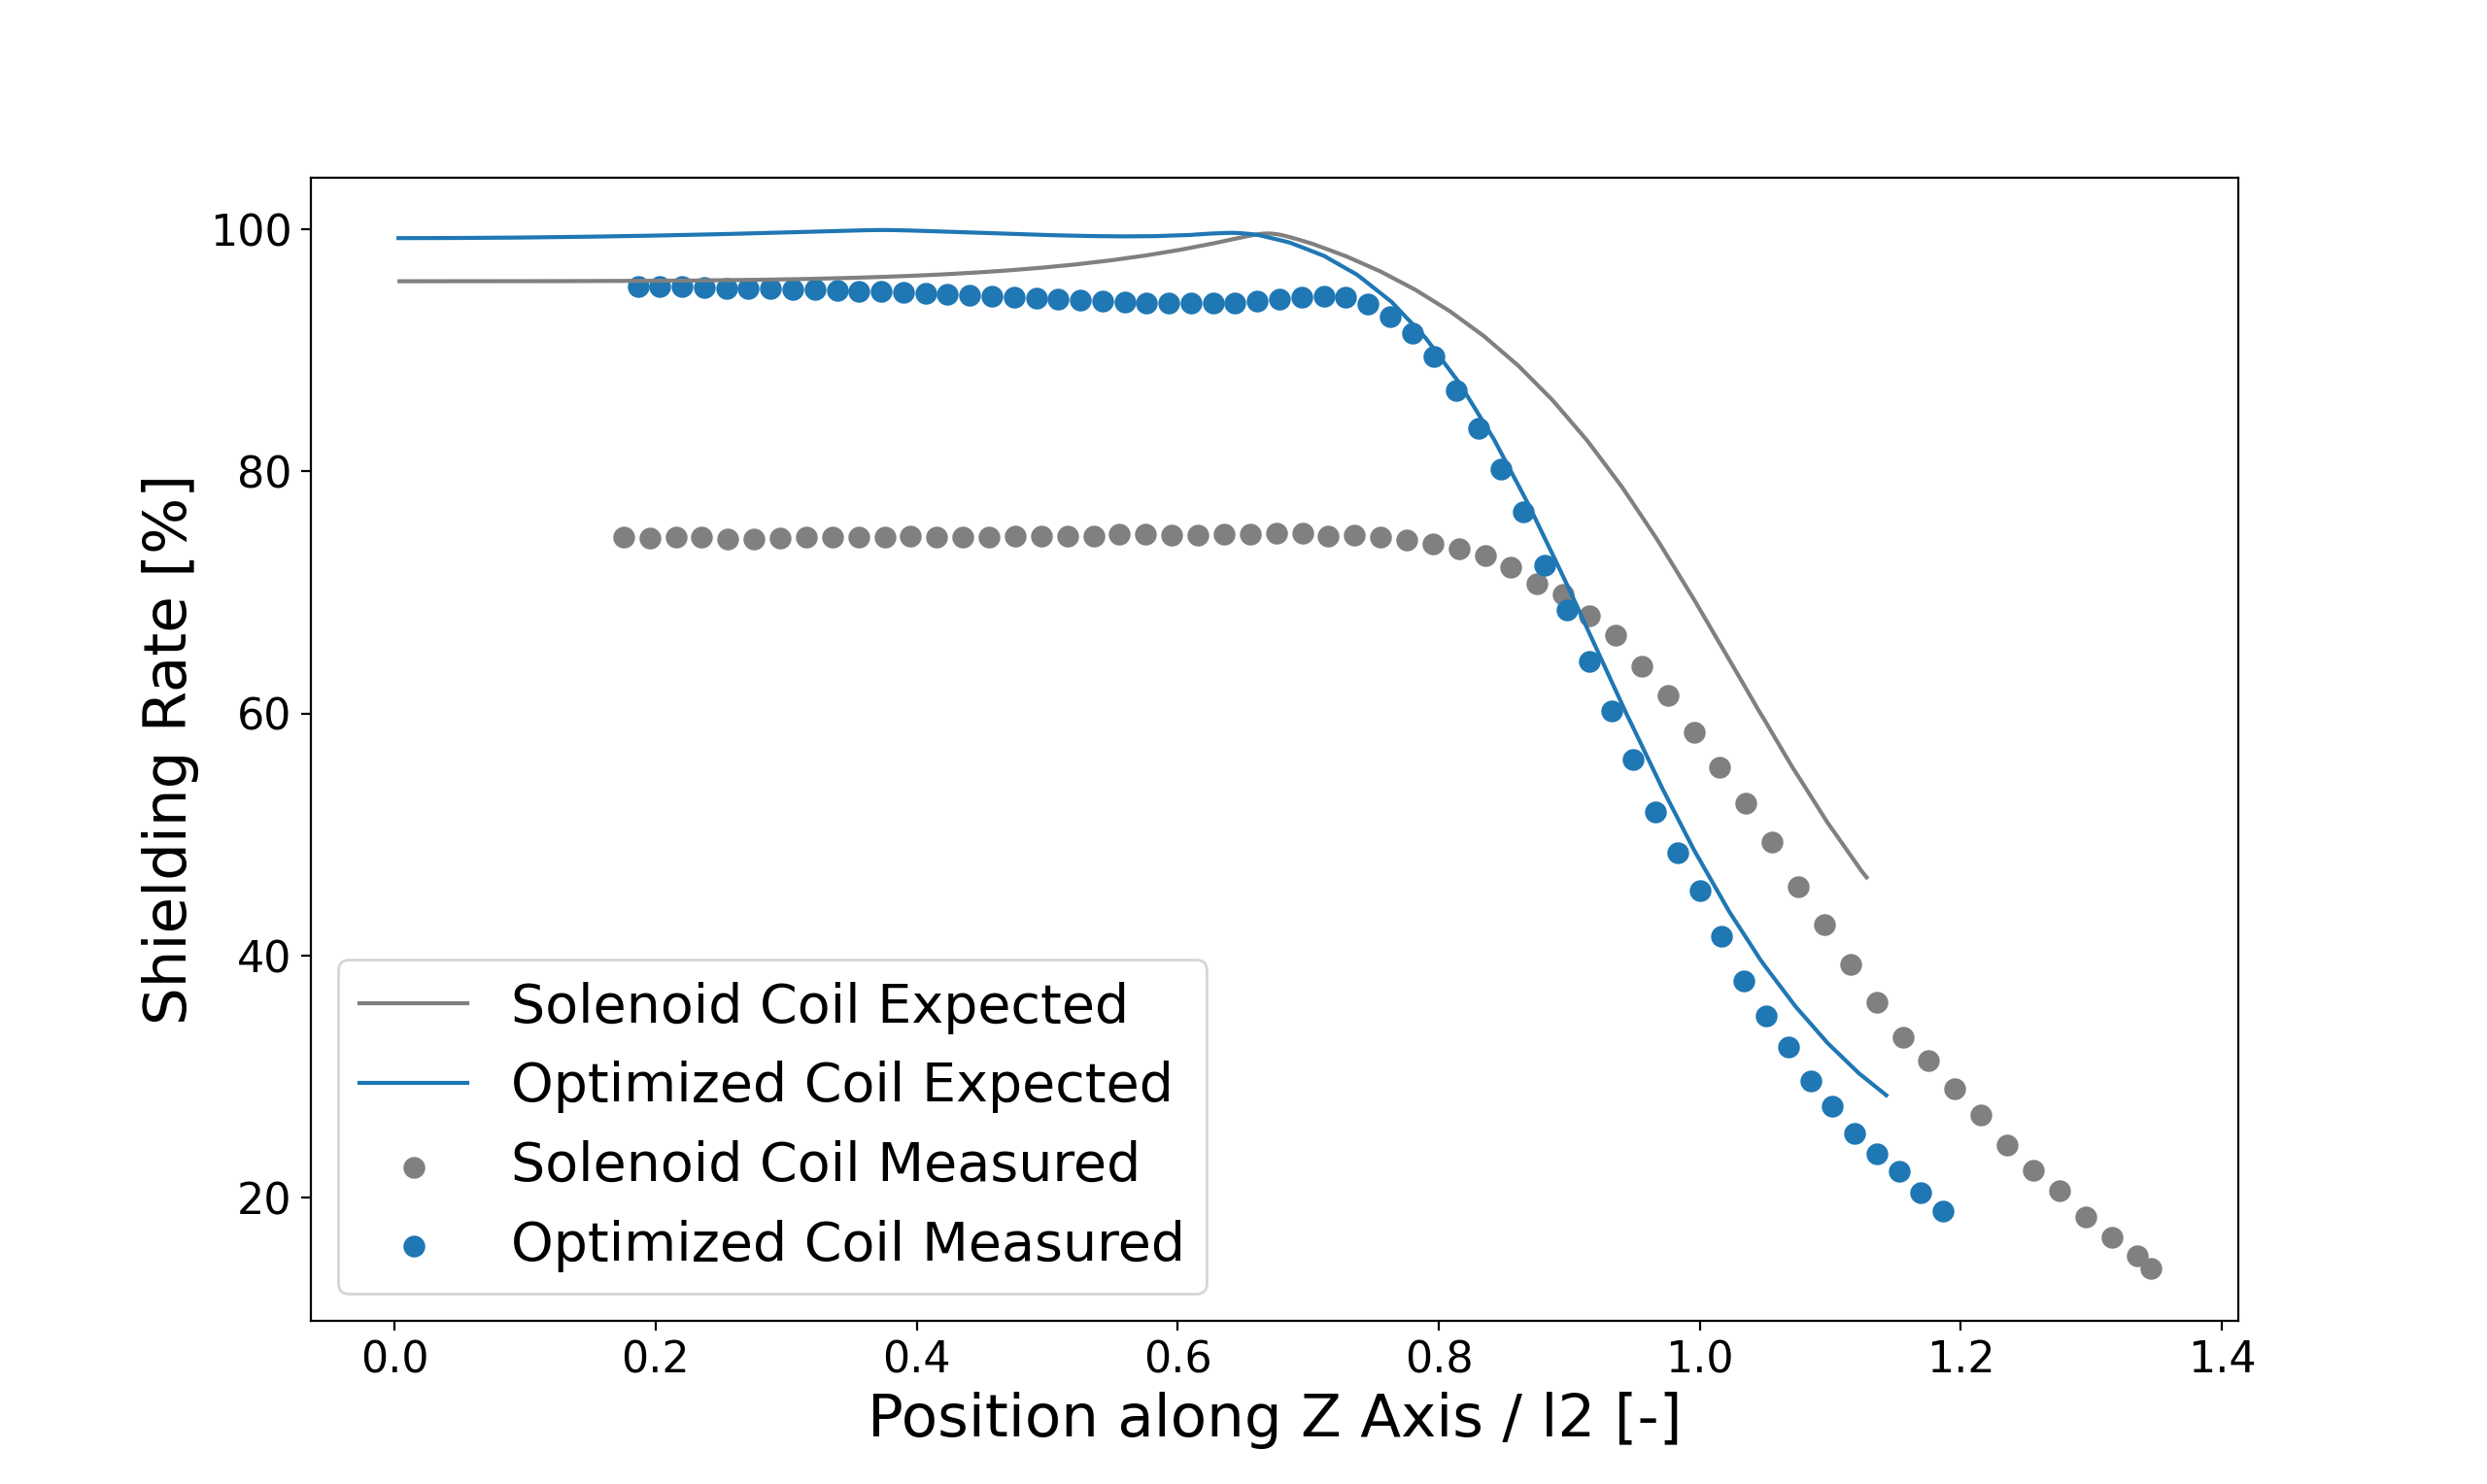
\includegraphics[width=18cm, bb=9 9 900 550]{./section4Optimal/combinedShieldingRates.png}
  \caption{Measured shielding rate along the central axis.}
  \label{fig:optimizedCoilExperimentResultCentral}
\end{figure}
\begin{figure}[H]
  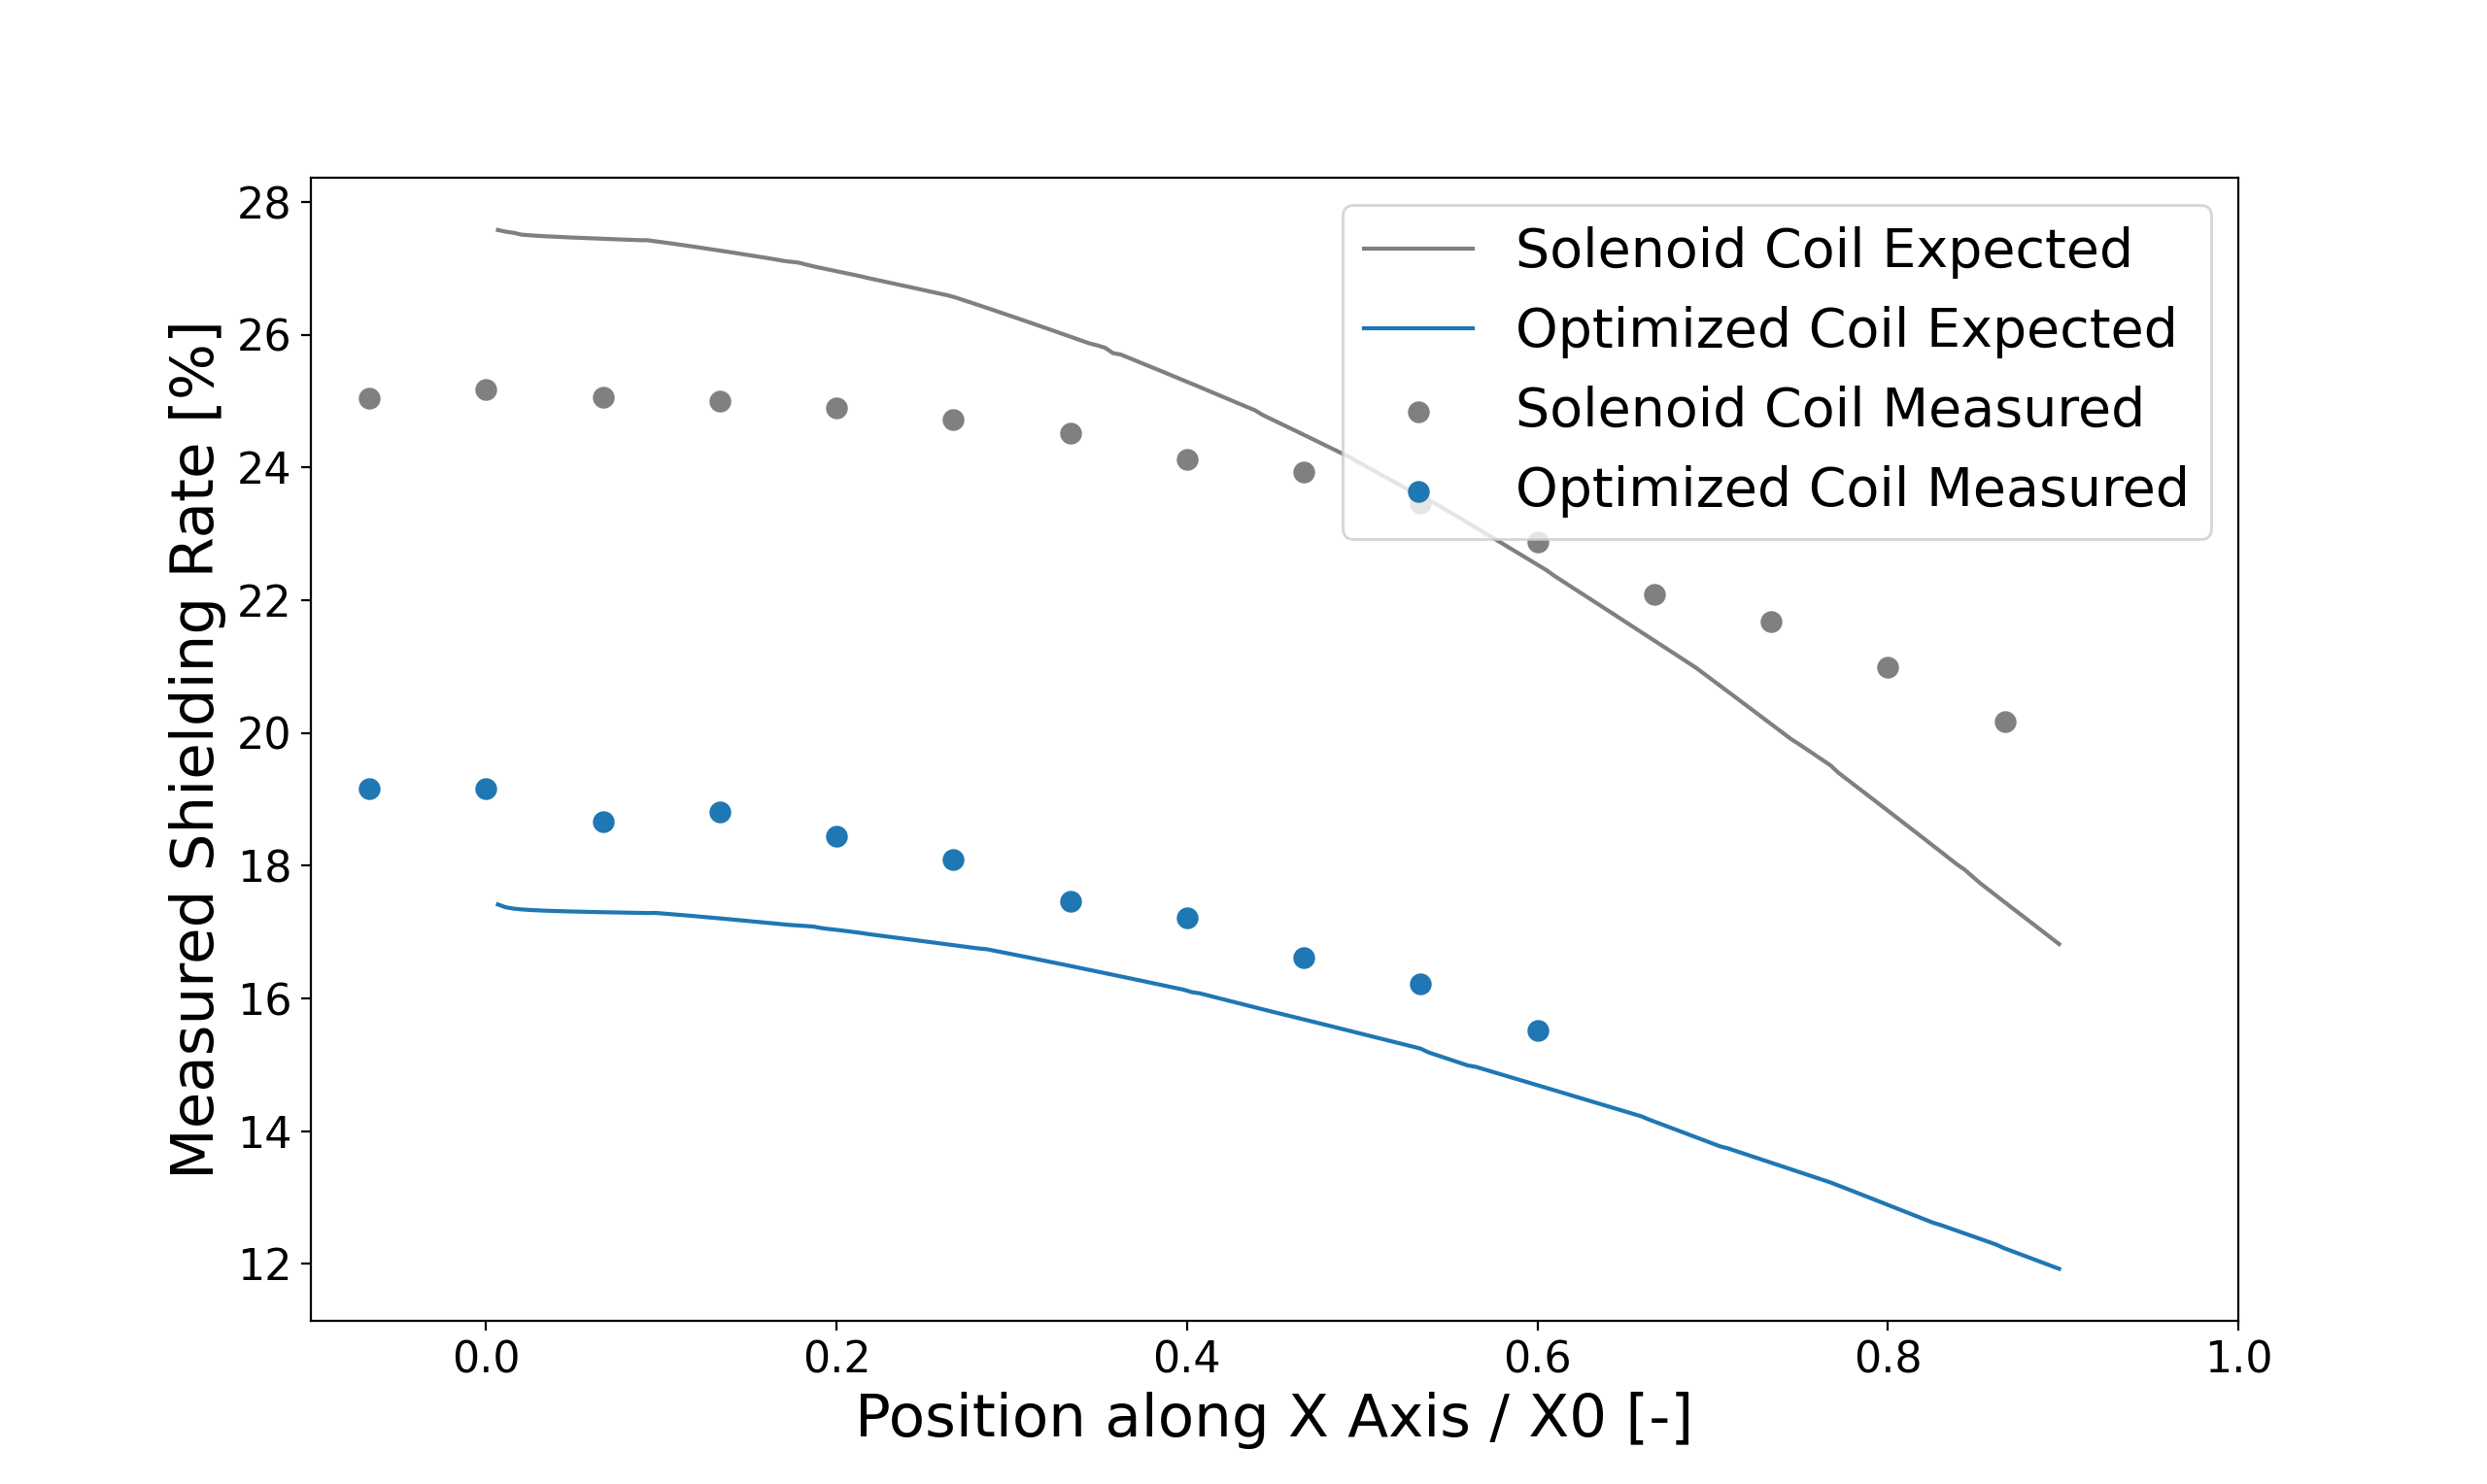
\includegraphics[width=18cm, bb=9 9 900 550]{./section4Optimal/combinedShieldingRatesTopLine.png}
  \caption{Measured shielding rate along the top line.}
  \label{fig:optimizedCoilExperimentResultTopLine}
\end{figure}
From Fig. \ref{fig:optimizedCoilExperimentResultCentral} we can see that for the inner field the optimized coil shows a better performance on shielding rates than the conventional solenoid,
and for the outer field the optimized coil the optimized coil reinforced the outer field.


\subsubsection{Conclusion}
In this section, we have show the result of our study on the optimized position a superconductor windings can be.
Through the simulation and experiment,
we have found that:
\begin{enumerate}
  \item Placing more turns near the edge increases the shielding rate, since the overshielding observed on a solenoid coil is released.
  \item Give the coil some margin on the edge reduces the disturbtion on the external field.
  This conclusion is considered reasonable due to the fact that $B$ field decays proportionally to $1r^2$.
\end{enumerate}


\subsection{Optimal Position of Ferromagnets}
In this section, we denote the optimal position of the ferromagnet.
As the above, the purpose, the theory, the method and finally the result would be denoted.


\subsubsection{Purpose}
The question about how to place the ferromagnet remains open.
The purpose of this section is to figure out figure out the best position of ferromagnets to achieve the best cloaking performance.


\subsubsection{Theory}
To translate the problem into mathmetical description,
we have first approximated the position of forromagnets by a four degree polynomial distribution function which denotes the corresponding $\rho$ components from the given $z$ components.
\begin{eqnarray}
  \rho_m(z_m|\mathbf{w}) = w_0 + w_1z_m + w_2z_m^2 + w_3z_m^3 + w_4z_m^4 + w_5z_m^5\\
  z_m \in \mathrm{[}0.5Z_0, 1.5Z_0\mathrm{]}\nonumber
\end{eqnarray}
where $Z_0$ represents the half length of the inner coil or the coil's top edge position,
$\rho_m$ represents the $\rho$ components of the ferromagnet,
$z_m$ represents the $z$ components of the ferromagnet,
$\mathbf{w}$ represents the weights of each term, which is the variable.
In this way, the optimization problem can be written in mathmetical form shown below.
\begin{eqnarray}
  \mathrm{variable}&:& \mathbf{w} = \{w_0, w_1, w_2, w_3, w_4, w_5\}\\
  \mathrm{loss\quad function}&:& f(\mathbf{w}) = mean\left(|\mathbf{B}_{in}(\mathbf{x})|\right) / mean\left(|\mathbf{B}_{out}(\mathbf{x})|\right)\\\nonumber
  \mathrm{constraint1}&:& g_1(\mathbf{w}) = \rho_m(\mathbf{w}|z_m=1.5Z_0) = -\left(w_0 + w_1(1.5Z_0) + ... + w_5(1.5Z_0)^5\right)\\\nonumber
  \mathrm{constraint2}&:& g_2(\mathbf{w}) = \rho_m(\mathbf{w}|z_m=0.5Z_0) = \left(w_0 + w_1(0.5Z_0) + ... + w_5(0.5Z_0)^5 \le \rho_0 \right) \le0\nonumber
\end{eqnarray}
The loss function can be anything which has minimum value when the inner field minimizes and the our field maximizes.
Constraints are aimed to limit the distribution function lies near the coil,
which guarantees the solution to have reasonable physical meaning.
The problem can be seen as a {\sl continuous constrained linear} optimization problem,
since the main variable $\mathbf{w}$ takes continuous values,
the polynomial is linear to $\mathbf{w}$.
This kind of optimization problem can be solved by the conventional method of Lagrange multiplier under Karush-Kuhn-Tucker(KKT) condition,
by introducing the Lagrange function:
\begin{eqnarray}
  Lagrange Function \nabla L(\mathbf{w, \lambda}) = \nabla\left( f(\mathbf{w})+\lambda_1 g_1(\mathbf{w})+\lambda_2 g_2(\mathbf{w})\right)=0
\end{eqnarray}
All left is to solve the simultaneous equations of the KKT condition.
\begin{eqnarray}
  \frac{\partial L}{\partial w_0}&=&\frac{\partial}{\partial w_0}f(\mathbf{w})+\lambda_1(-1)+\lambda_2(1)=0\\
  \frac{\partial L}{\partial w_1}&=&\frac{\partial}{\partial w_1}f(\mathbf{w})+\lambda_1(-1.5Z_0)+\lambda_2(0.5Z_0)=0\\\nonumber
  \frac{\partial L}{\partial w_2}&=&\frac{\partial}{\partial w_2}f(\mathbf{w})+\lambda_1(-(1.5Z_0)^2)+\lambda_2((0.5Z_0)^2)=0\\\nonumber
  &.&..\\\nonumber
  \frac{\partial L}{\partial \lambda_1}&=&g_1(\mathbf{w})=0\\\nonumber
  \frac{\partial L}{\partial \lambda_2}&=&g_2(\mathbf{w})=0\nonumber
\end{eqnarray}

However, this requests the first derivate of $f(\mathbf{w})$ which we don't have.
Therefore, we have used an iterative method to solve the equations, the schametic procedure is shown below.
\begin{eqnarray}
  w_0^{(k+1)} = w_0^{(k)} - \alpha\frac{\partial f(w^{(k)})}{\partial w_0}\\
  w_1^{(k+1)} = w_1^{(k)} - \alpha\frac{\partial f(w^{(k)})}{\partial w_1}\\\nonumber
  ...\\\nonumber
  w_5^{(k+1)} = w_5^{(k)} - \alpha\frac{\partial f(w^{(k)})}{\partial w_5}\nonumber
\end{eqnarray}
where the derivate part $\frac{\partial f(w^{(k)})}{\partial w_0}$ is substituded by numerical derivate.


\subsubsection{Method}
The optimization procedure is shown below
\begin{enumerate}
  \item Randomly choose $\mathbf{w}$, which defines the initial distribution of the ferromagnet.
  \item Calculate derivate of f $f(\mathbf{w+\pm \Delta})$.
  \item Update $\mathbf{w}$ to the direction minimizing $f$.
  \item Repeat until $\mathbf{w}$ is not improving.
\end{enumerate}
For the calculation of the inner and outer field,
finite element method is used.
To reduce the calculation time, we have neglect the nonlinear permeability generally seen in ferromagnet
and used a fix permeability of 100,
which is relatively small but is just fine to give us the strong magnetization under the current condition.
For the optimization algorithm, we have chosen the trust-constraint algorithm,
which belongs to the quasi-newton method of optimization.
The detail specification used in the calculation is shown in Fig. \ref{fig:FMEvaluationRegion} and Tab. \ref{tab:FMSpecification}.
\begin{figure}[H]
  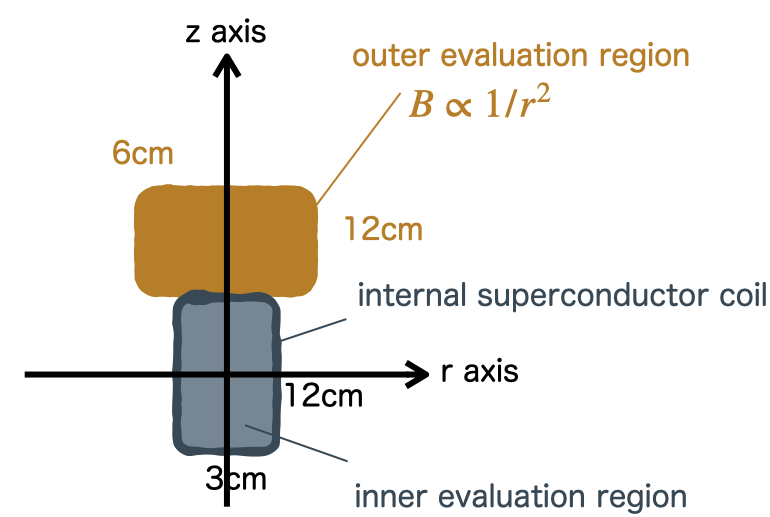
\includegraphics[width=18cm, bb=9 9 900 600]{./section4Optimal/evaluationRegion.png}
  \caption{Evaluation region.}
  \label{fig:FMEvaluationRegion}
\end{figure}
\begin{table}[H]
  \centering
  \caption{Specification of the ferromagnet optimization.}
  \label{tab:FMSpecification}
  \begin{tabular}{cc}\hline\hline
    Thickness of Ferromagnet & 1 [mm]\\
    Relative Permeability & 100 (fix)\\
    Loss Function & average inner field / average outer field\\\hline\hline
  \end{tabular}
\end{table}


\subsubsection{Result and Discussion}
The result of the optimization progress is shown in Fig. \ref{fig:FMOptimization}.
\begin{figure}[H]
  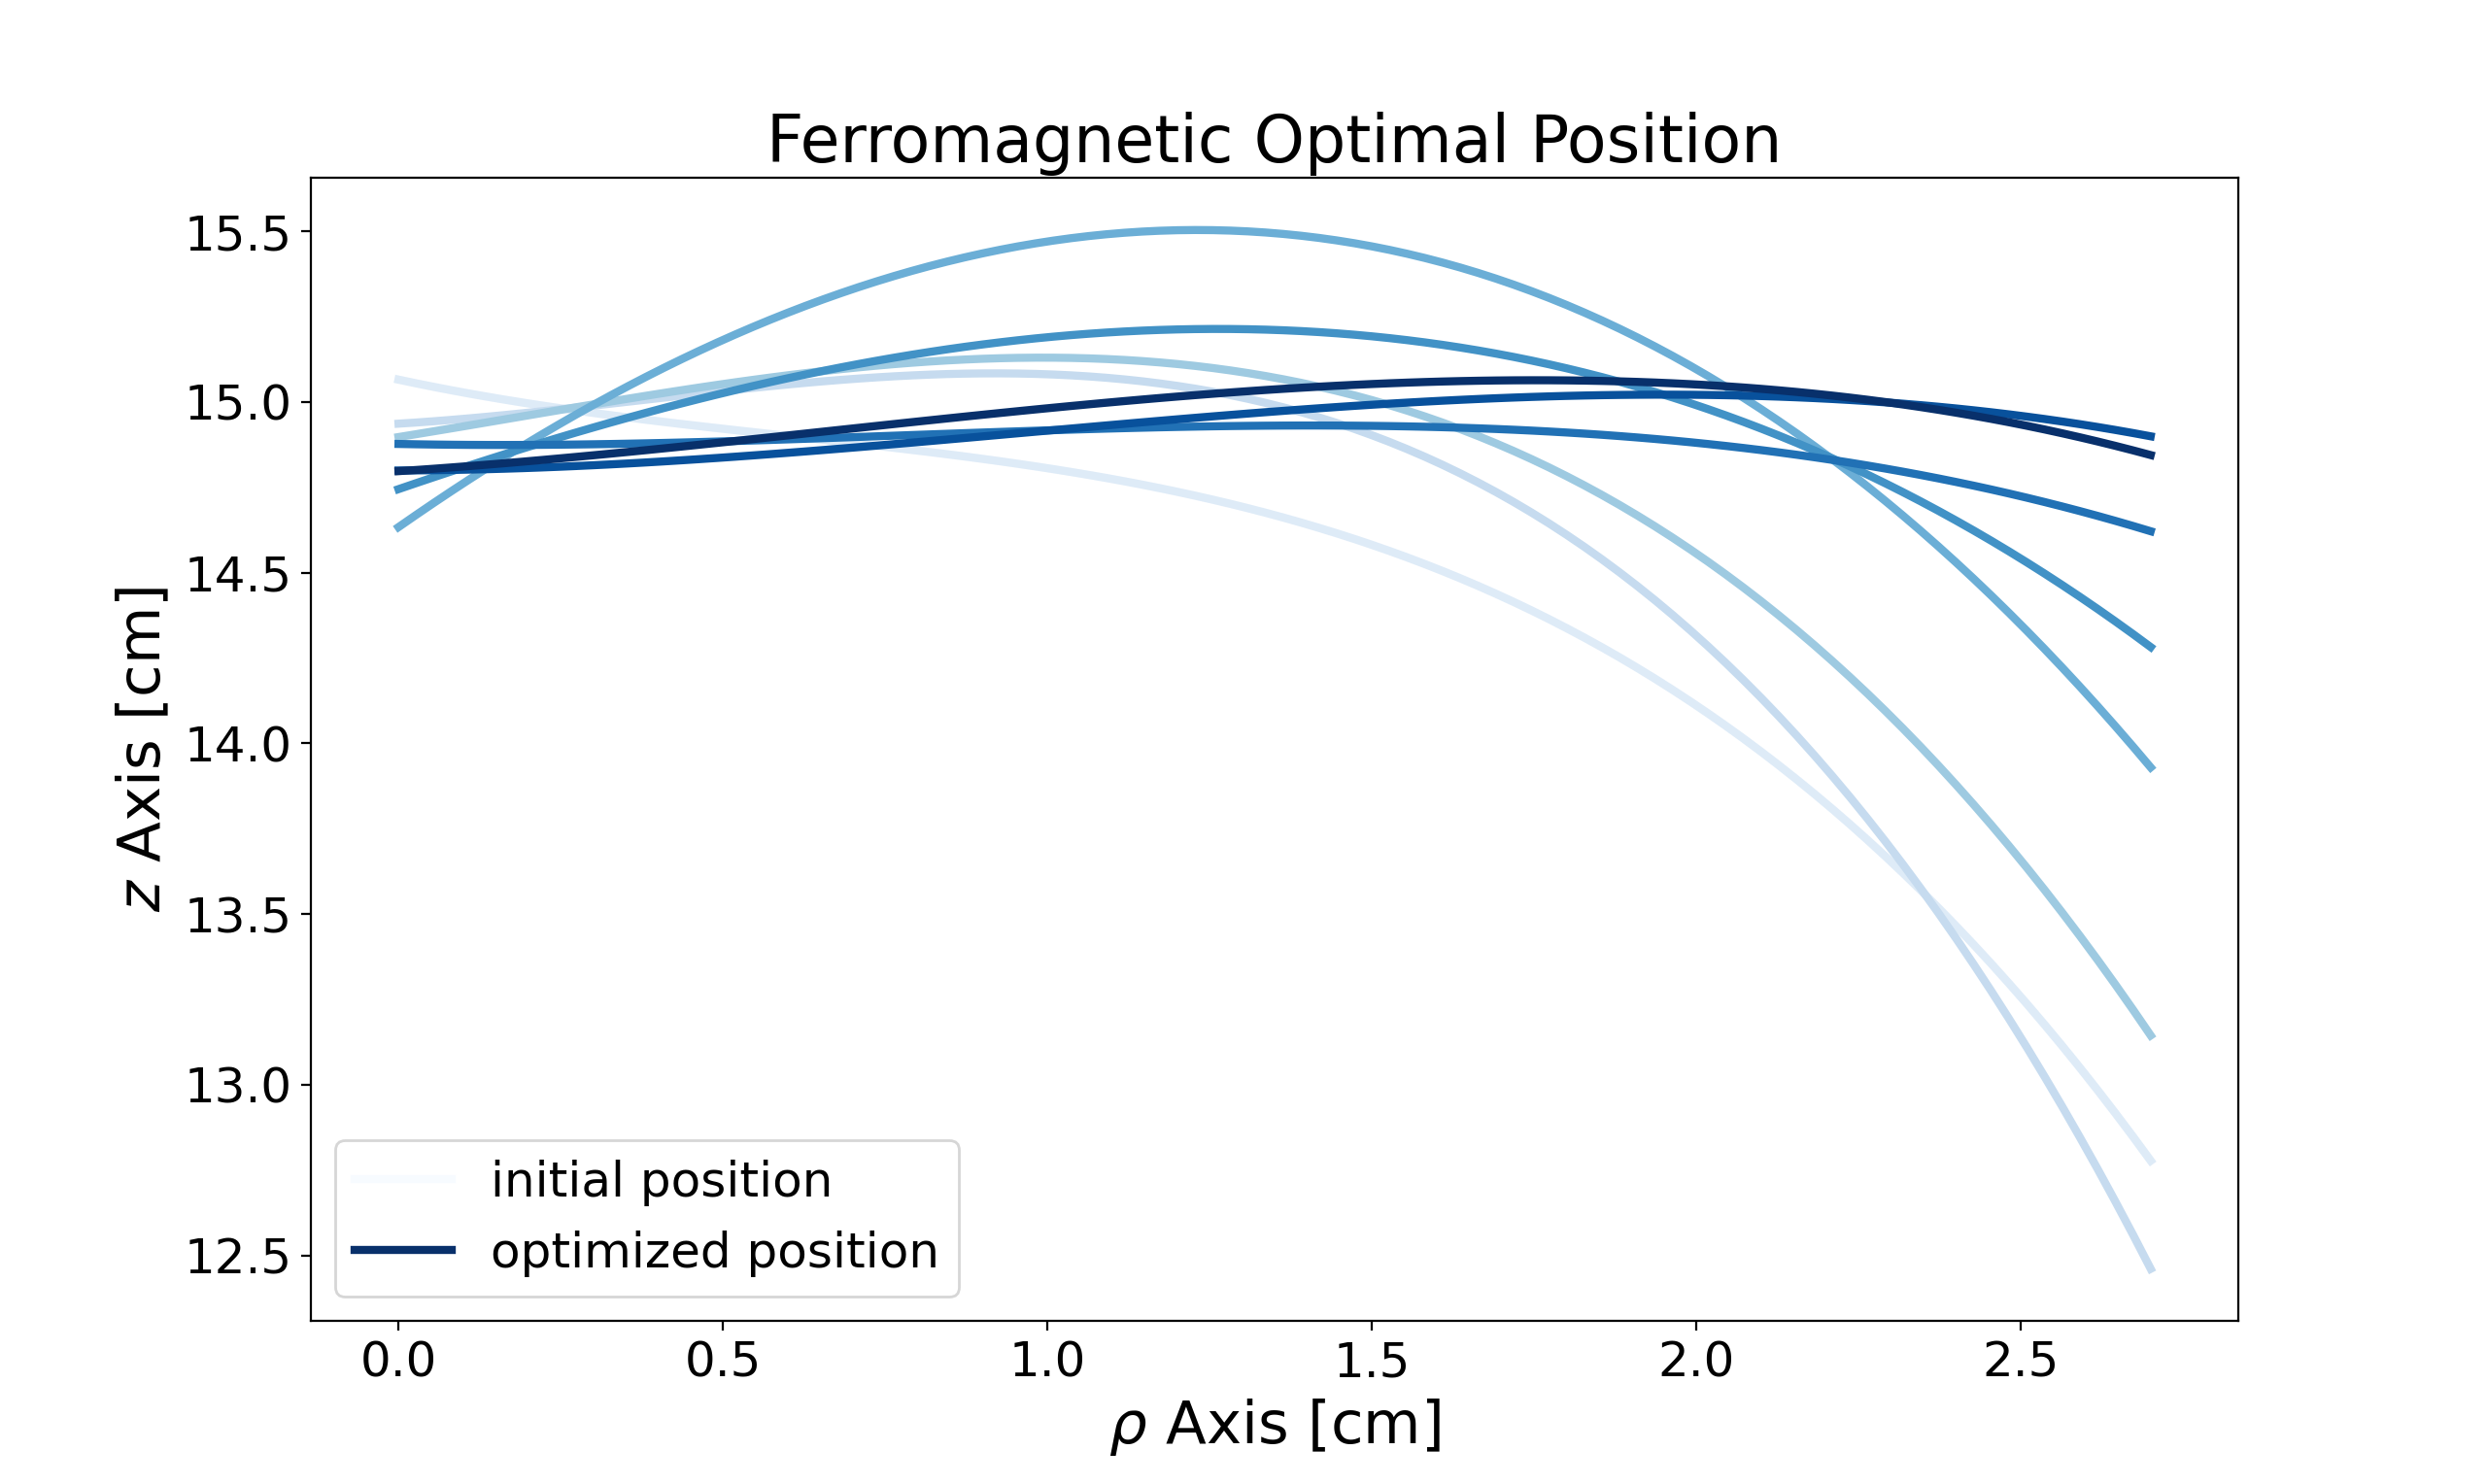
\includegraphics[width=18cm, bb=9 9 900 550]{./section4Optimal/FMOptimization.png}
  \caption{Optimization progress.}
  \label{fig:FMOptimization}
\end{figure}
In Fig. \ref{fig:FMOptimization}, the optimization have started from the lightest line, then the darker,
finally the darkest line which lies almost flat on the edge of the internal coil.
The result indicates that the best position of the ferromagnet to be placed is about flat on the edge.

To confirm this result, the magnetic field distribution near the coil is shown below,
with the comparison of whether the ferromagnet is included.
\begin{figure}[H]
  \includegraphics[width=18cm, bb=9 9 900 550]{./section4Optimal/FMDistribution.png}
  \caption{The $B$ field distribution in situations (a) without ferromagnet (b) with ferromagnet.}
  \label{fig:FMDistribution}
\end{figure}
\begin{figure}[H]
  \includegraphics[width=18cm, bb=9 9 900 550]{./section4Optimal/FMDistributionTopLine.png}
  \caption{The $B$ field distribution on top line.}
  \label{fig:FMDistribution}
\end{figure}
From \ref{fig:FMDistribution} we can find that the external field distribution around the top edge of the inner coil is reinceforced when the ferromagnet is placed on the optimized position.
Also, if we look into the field on the ferromagnet carefully,
one can find that the ferromagnet is generating field over 1 T,
which is considered impossible in practice.
This results from the neglection of the nonlinear permeability of the ferromagnet.
Ferromagnets usually have maximum magnetization around 700 mT.
Instead of taking this limitation into consideration, which would have a bad impact on the convergence,
we approach it using a fix permeability,
which is a linear model thus can generate magnetization over the expected.
This may seem a bad idea, but since we are facing a condition that
the ferromagnet being placed under a very strong field of several Tesla exceeding the maximum magnetization,
the optimized result in our simulation can be explained as the best position at which the ferromagnet performs its maximum magnetization.
Therefore, this result is considered correct in strong fields.

However, this result has also exposed the problem of our proposed Electromagnetic Induction Type Magnetic Cloak,
which is,
the cloaking ability relying on the maximum magnetization of the ferromagnet.
Since this model uses ferromagnet to compensate the outer field near the coil edge,
the maximum fields it can generate is determined by the maximum magnetization of the ferromagnet.
For instance, a magnet having maximum 700 mT magnetization cannot compensate more than about 10\% of the outer field when it is imposed by 10 T magnetic field.
In our case of the spaceuseage, only a 2 T field is needed so that the proposal should be appliable,
but when it comes to other case in which 10 T or 20 T shielding is requested,
the cloaking ability cannot be achieved.
Of course, even in the cases with imposed field above 10 T, a satisfying shielding ability can be expected since the superconductor should work problemlessly.


\subsubsection{Conclusion}
In this chapter,
we have denoted the optimized position of placing the ferromagnet such that the inner field can be minimized and the outer field can be maximized.
After our calculation, the best position is found to be almost flat on the edge,
which have the scalability to much more field.
Howver, the provided magnetization is limited by the maximum magnetization the ferromagnet can provide,
which is mostly up to 700 mT.


\newpage
\begin{thebibliography}{20}
  \bibitem{2_1} Dirk P. Kroese, "Handbook of Monte Carlo Methods", Wiley Series in Probability and Statistics (2014)
\end{thebibliography}



% \section{Experiment under 1T Environment}
% \subsection{Purpose}
% \subsection{Theory}
% \subsection{Methods}
% \subsection{Results}
% \subsection{Discussion}
% \subsection{Conclusion}

\newpage
\section{Conclusion}
% section 5 conclusion
In this thesis, we have dedicated in developing a shielding system which is able to operate under high magneitc field environment and have enough "cloak" ability.
The target is set to be spaceusage in which the system is required to work under 1 T field and not weakening the outer field due to the invasion of comic rays.
During our investigation,
we have proposed the Electromagnetic Induction Type Magnetic Cloak,
which combines the high temperature superconductor tape and the ferromagnet to achieve shielding and cloaking ability.
Briefly speaking, the structure is to place a ferromagnets on the edge of the a superconducting coil,
of which the detail is shown in chapter 2.

Through our study on the effectiveness of EIMC, denoted in chapter 3,
we have prooved three points:
\begin{enumerate}
  \item The time constant should be at least a few years, which allowing the system to shield high stable magnetic fields.
  \item The scaled down model shows a shielding ability of over 90\%, from which shielding ability near 100\% in full scale model can be expected.
  \item Inserting ferromagnet is able to reinforce the external field near the coil edge, which reduces the probability of comic rays penetrating into the space craft.
\end{enumerate}
Throug the study in chapter 4, we are able to reveal some guidelines on the construction according to the optimization calculation, which are:
\begin{enumerate}
  \item For the superconductor windings, the shielding rates can be achieved by placing more turns on the edge. On the other hand,
  reducing the length of the coil may achieve a higher cloaking property,
  reinforcing the outer field nearby.
  \item For the ferromagnet, it is considered the best to be placed almost flat on the edge of the coil.
  Since the system works under high fields, the ones having maximum magnetization is considered better when chosing between different ferromagnets made of different material,
  while the permeability is the secondary parameter with a lower priority.
\end{enumerate}

Finally, we are able to answer the foundemantal question:
Can magnetic cloak under high fields be achieved?
Our answer is: conditionally afirmative.
Although good shielding ability can be expected, the property of not disturbing external field is limited by the maximum magnetization.
The stronger magnet is applied, the higher cloaking ability can be achieved.


\newpage
\section*{Acknowledgments}
% Acknowledgments
I am grateful to Prefessor Makoto Tsuda for helpful discussions and comments on the slides,
along with Assistant Professor Yoh Nagasaki for his outstanding ideas.
Past and present members of our laboratory should not be missed for their participation in seminars and advises on Job hunting.
Masaki Maruyama, Daichi Wakamatsu, Yuuki Ichijou, Yu Yoshimura, Kannta Sawada and all the other members, thank you.

Beyond Tohoku University members,
I appreciate Mr. Ko Hsiao-Min, Yokohama National University for his thoughtful advises on the philosophy of life,
my girlfirend Megumi Baba for her dedicated support and exchanging experiences on difficult hierarchical relationship,
and my parents for their sincere support.

I personally express my sincere thanks to Japan-Taiwan Exchange Association for their scholarship.
It is their support that brings me the extraordinary life being a foreign researcher in Japan.

Finally, this work is sponser under the Grant-in-Aid for Young Scientists project (No. JP19K15204) by the Ministry of Education, Culture, Sports, Science and Technology, Japan.
Without their funding support,
we would not have completed the most of our experiments and simulation.


\end{document}


% \begin{thebibliography}{7}
%   \bibitem{1_1_1} N. Miura, T. Goto, K. Nakao, S. Takeyama, T. Sakakibara, T. Haruyama, T. Kikuchi, "Production of ultra-high magnetic fields and their application to solid state physics", Physica B: Condensed Matter, Volume 155, Issues 1\UTF{2013}3, Pages 23-32 (1989)
%   \bibitem{1_1_2} Filippo Ambroglini1, Roberto Battiston2 and William J. Burger, "Evaluation of Superconducting Magnet Shield Configurations for Long Duration Manned Space Missions", Frontiers in Oncology, Vol. 6, p. 97 (2016)
%   \bibitem{1_1_3} R. Musenich, V. Calvelli, S. Farinon, W. J. Burger, R. Battiston, "Space Radiation Superconducting Shields", Journal of Physics: Conference Series 507 032033 (2014)
%   \bibitem{1_1_4}
%   \bibitem{1_1_5}
%   \bibitem{1_2_1} Francis A. Cucinotta, "Space Radiation Risks for Astronauts on Multiple International Space Station Missions", PLoS ONE 9(4): e96099 (2014)
%
%   \bibitem{1_10} R.Musenich et al., "Space Radiation Superconducting Shields", Journal of Physics: Conference Series 507 (2014) 032033
% \end{thebibliography}
